\documentclass[sigconf,review,10pt,acmthm=false]{acmart}
% MobiSys 2027 submission: single-blind, 12-page body limit (references + appendix excluded).

\usepackage{booktabs}
\usepackage{array}
\usepackage{amsmath,amsthm}   % acmart: do NOT load amssymb (clashes with newtx \Bbbk)
\usepackage{graphicx}
\usepackage{xcolor}
\usepackage{xspace}
\xspaceaddexceptions{\% \,}
\usepackage{algorithm}
\usepackage[noend]{algpseudocode}
\usepackage{tikz}
\usetikzlibrary{arrows.meta,positioning,calc,shapes.misc,decorations.pathreplacing,backgrounds,fit}
\usepackage{pgfplots}
\pgfplotsset{compat=1.17} % use 1.18 on TL>=2021
% matured-style.tex -- shared table/plot look for the MobiSys 2027 papers (same palette as the Figure 1 comics).
% Copy into each manuscript and % matured-style.tex -- shared table/plot look for the MobiSys 2027 papers (same palette as the Figure 1 comics).
% Copy into each manuscript and % matured-style.tex -- shared table/plot look for the MobiSys 2027 papers (same palette as the Figure 1 comics).
% Copy into each manuscript and \input{matured-style} after xcolor/booktabs/pgfplots are loaded.
% Muted, print-safe colours; series also differ by marker/dash so the plots survive greyscale.
\usepackage{colortbl}
% ---- palette -----------------------------------------------------------------
\definecolor{mInk}{HTML}{2B2A29}
\definecolor{mSlate}{HTML}{5E6670}
\definecolor{mNavy}{HTML}{2F3E55}
\definecolor{mTeal}{HTML}{2F6F68}
\definecolor{mSage}{HTML}{5F8A68}
\definecolor{mOchre}{HTML}{B9873A}
\definecolor{mBrick}{HTML}{9E4A3C}
\definecolor{mPlum}{HTML}{5B3F66}
\definecolor{mHead}{HTML}{E9ECEF}   % table header fill
\definecolor{mGroup}{HTML}{F3F1EC}  % group/section row fill
\definecolor{mHiB}{HTML}{F4E3DF}    % brick tint: bad/unsafe cell
\definecolor{mHiT}{HTML}{DFEDEA}    % teal tint: good/safe cell
\definecolor{mHiO}{HTML}{F6EBD6}    % ochre tint: emphasis
% ---- tables ------------------------------------------------------------------
% \mhead   : first command of a header row  -> shaded header
% \mgroup{n}{text} : full-width shaded group label row spanning n columns
% \mbad{x} \mgood{x} \mhi{x} : tinted cells (colortbl \cellcolor)
\newcommand{\mhead}{\rowcolor{mHead}}
% shaded rows overhang by \tabcolsep, so shaded tables keep the outer \tabcolsep (no @{} at the edges)
\newcommand{\mgroup}[2]{\rowcolor{mGroup}\multicolumn{#1}{l}{\textit{#2}}\\}
\newcommand{\mbad}[1]{\cellcolor{mHiB}#1}
\newcommand{\mgood}[1]{\cellcolor{mHiT}#1}
\newcommand{\mhi}[1]{\cellcolor{mHiO}#1}
\newcommand{\mtab}{\footnotesize\setlength{\tabcolsep}{3.6pt}\renewcommand{\arraystretch}{1.05}}
\setlength{\aboverulesep}{0.25ex}\setlength{\belowrulesep}{0.4ex}
\setlength{\heavyrulewidth}{0.08em}\setlength{\lightrulewidth}{0.05em}
% ---- plots -------------------------------------------------------------------
\pgfplotscreateplotcyclelist{matured}{%
  {mBrick,mark=*,mark size=1.4pt},
  {mTeal,mark=square*,mark size=1.3pt},
  {mOchre,mark=triangle*,mark size=1.7pt},
  {mNavy,mark=diamond*,mark size=1.7pt},
  {mSage,mark=pentagon*,mark size=1.5pt},
  {mPlum,mark=o,mark size=1.4pt}}
\pgfplotscreateplotcyclelist{maturedbars}{%
  {fill=mBrick,draw=mInk!75},{fill=mTeal,draw=mInk!75},{fill=mOchre,draw=mInk!75},
  {fill=mNavy,draw=mInk!75},{fill=mSage,draw=mInk!75},{fill=mPlum,draw=mInk!75}}
\pgfplotsset{
  matured/.style={
    cycle list name=matured,
    every axis plot/.append style={line width=0.9pt},
    axis x line*=bottom, axis y line*=left,
    axis line style={draw=mSlate!80, line width=0.5pt},
    every tick/.style={draw=mSlate!80, line width=0.4pt}, tick align=outside, major tick length=2pt,
    ymajorgrids, major grid style={draw=mSlate!18, line width=0.35pt},
    tick label style={font=\footnotesize, text=mInk},
    label style={font=\footnotesize, text=mInk},
    title style={font=\footnotesize\bfseries, text=mInk, yshift=-1ex},
    legend style={font=\footnotesize, draw=none, fill=white, fill opacity=0.85, text opacity=1,
                  legend cell align=left, column sep=4pt},
    legend image post style={line width=0.9pt},
    error bars/error bar style={line width=0.5pt},
    error bars/error mark options={rotate=90, mark size=1.4pt, line width=0.5pt},
  },
  maturedbar/.style={matured, ybar, bar width=5pt, enlarge x limits=0.12, cycle list name=maturedbars,
    every axis plot/.append style={line width=0.4pt}},
}
 after xcolor/booktabs/pgfplots are loaded.
% Muted, print-safe colours; series also differ by marker/dash so the plots survive greyscale.
\usepackage{colortbl}
% ---- palette -----------------------------------------------------------------
\definecolor{mInk}{HTML}{2B2A29}
\definecolor{mSlate}{HTML}{5E6670}
\definecolor{mNavy}{HTML}{2F3E55}
\definecolor{mTeal}{HTML}{2F6F68}
\definecolor{mSage}{HTML}{5F8A68}
\definecolor{mOchre}{HTML}{B9873A}
\definecolor{mBrick}{HTML}{9E4A3C}
\definecolor{mPlum}{HTML}{5B3F66}
\definecolor{mHead}{HTML}{E9ECEF}   % table header fill
\definecolor{mGroup}{HTML}{F3F1EC}  % group/section row fill
\definecolor{mHiB}{HTML}{F4E3DF}    % brick tint: bad/unsafe cell
\definecolor{mHiT}{HTML}{DFEDEA}    % teal tint: good/safe cell
\definecolor{mHiO}{HTML}{F6EBD6}    % ochre tint: emphasis
% ---- tables ------------------------------------------------------------------
% \mhead   : first command of a header row  -> shaded header
% \mgroup{n}{text} : full-width shaded group label row spanning n columns
% \mbad{x} \mgood{x} \mhi{x} : tinted cells (colortbl \cellcolor)
\newcommand{\mhead}{\rowcolor{mHead}}
% shaded rows overhang by \tabcolsep, so shaded tables keep the outer \tabcolsep (no @{} at the edges)
\newcommand{\mgroup}[2]{\rowcolor{mGroup}\multicolumn{#1}{l}{\textit{#2}}\\}
\newcommand{\mbad}[1]{\cellcolor{mHiB}#1}
\newcommand{\mgood}[1]{\cellcolor{mHiT}#1}
\newcommand{\mhi}[1]{\cellcolor{mHiO}#1}
\newcommand{\mtab}{\footnotesize\setlength{\tabcolsep}{3.6pt}\renewcommand{\arraystretch}{1.05}}
\setlength{\aboverulesep}{0.25ex}\setlength{\belowrulesep}{0.4ex}
\setlength{\heavyrulewidth}{0.08em}\setlength{\lightrulewidth}{0.05em}
% ---- plots -------------------------------------------------------------------
\pgfplotscreateplotcyclelist{matured}{%
  {mBrick,mark=*,mark size=1.4pt},
  {mTeal,mark=square*,mark size=1.3pt},
  {mOchre,mark=triangle*,mark size=1.7pt},
  {mNavy,mark=diamond*,mark size=1.7pt},
  {mSage,mark=pentagon*,mark size=1.5pt},
  {mPlum,mark=o,mark size=1.4pt}}
\pgfplotscreateplotcyclelist{maturedbars}{%
  {fill=mBrick,draw=mInk!75},{fill=mTeal,draw=mInk!75},{fill=mOchre,draw=mInk!75},
  {fill=mNavy,draw=mInk!75},{fill=mSage,draw=mInk!75},{fill=mPlum,draw=mInk!75}}
\pgfplotsset{
  matured/.style={
    cycle list name=matured,
    every axis plot/.append style={line width=0.9pt},
    axis x line*=bottom, axis y line*=left,
    axis line style={draw=mSlate!80, line width=0.5pt},
    every tick/.style={draw=mSlate!80, line width=0.4pt}, tick align=outside, major tick length=2pt,
    ymajorgrids, major grid style={draw=mSlate!18, line width=0.35pt},
    tick label style={font=\footnotesize, text=mInk},
    label style={font=\footnotesize, text=mInk},
    title style={font=\footnotesize\bfseries, text=mInk, yshift=-1ex},
    legend style={font=\footnotesize, draw=none, fill=white, fill opacity=0.85, text opacity=1,
                  legend cell align=left, column sep=4pt},
    legend image post style={line width=0.9pt},
    error bars/error bar style={line width=0.5pt},
    error bars/error mark options={rotate=90, mark size=1.4pt, line width=0.5pt},
  },
  maturedbar/.style={matured, ybar, bar width=5pt, enlarge x limits=0.12, cycle list name=maturedbars,
    every axis plot/.append style={line width=0.4pt}},
}
 after xcolor/booktabs/pgfplots are loaded.
% Muted, print-safe colours; series also differ by marker/dash so the plots survive greyscale.
\usepackage{colortbl}
% ---- palette -----------------------------------------------------------------
\definecolor{mInk}{HTML}{2B2A29}
\definecolor{mSlate}{HTML}{5E6670}
\definecolor{mNavy}{HTML}{2F3E55}
\definecolor{mTeal}{HTML}{2F6F68}
\definecolor{mSage}{HTML}{5F8A68}
\definecolor{mOchre}{HTML}{B9873A}
\definecolor{mBrick}{HTML}{9E4A3C}
\definecolor{mPlum}{HTML}{5B3F66}
\definecolor{mHead}{HTML}{E9ECEF}   % table header fill
\definecolor{mGroup}{HTML}{F3F1EC}  % group/section row fill
\definecolor{mHiB}{HTML}{F4E3DF}    % brick tint: bad/unsafe cell
\definecolor{mHiT}{HTML}{DFEDEA}    % teal tint: good/safe cell
\definecolor{mHiO}{HTML}{F6EBD6}    % ochre tint: emphasis
% ---- tables ------------------------------------------------------------------
% \mhead   : first command of a header row  -> shaded header
% \mgroup{n}{text} : full-width shaded group label row spanning n columns
% \mbad{x} \mgood{x} \mhi{x} : tinted cells (colortbl \cellcolor)
\newcommand{\mhead}{\rowcolor{mHead}}
% shaded rows overhang by \tabcolsep, so shaded tables keep the outer \tabcolsep (no @{} at the edges)
\newcommand{\mgroup}[2]{\rowcolor{mGroup}\multicolumn{#1}{l}{\textit{#2}}\\}
\newcommand{\mbad}[1]{\cellcolor{mHiB}#1}
\newcommand{\mgood}[1]{\cellcolor{mHiT}#1}
\newcommand{\mhi}[1]{\cellcolor{mHiO}#1}
\newcommand{\mtab}{\footnotesize\setlength{\tabcolsep}{3.6pt}\renewcommand{\arraystretch}{1.05}}
\setlength{\aboverulesep}{0.25ex}\setlength{\belowrulesep}{0.4ex}
\setlength{\heavyrulewidth}{0.08em}\setlength{\lightrulewidth}{0.05em}
% ---- plots -------------------------------------------------------------------
\pgfplotscreateplotcyclelist{matured}{%
  {mBrick,mark=*,mark size=1.4pt},
  {mTeal,mark=square*,mark size=1.3pt},
  {mOchre,mark=triangle*,mark size=1.7pt},
  {mNavy,mark=diamond*,mark size=1.7pt},
  {mSage,mark=pentagon*,mark size=1.5pt},
  {mPlum,mark=o,mark size=1.4pt}}
\pgfplotscreateplotcyclelist{maturedbars}{%
  {fill=mBrick,draw=mInk!75},{fill=mTeal,draw=mInk!75},{fill=mOchre,draw=mInk!75},
  {fill=mNavy,draw=mInk!75},{fill=mSage,draw=mInk!75},{fill=mPlum,draw=mInk!75}}
\pgfplotsset{
  matured/.style={
    cycle list name=matured,
    every axis plot/.append style={line width=0.9pt},
    axis x line*=bottom, axis y line*=left,
    axis line style={draw=mSlate!80, line width=0.5pt},
    every tick/.style={draw=mSlate!80, line width=0.4pt}, tick align=outside, major tick length=2pt,
    ymajorgrids, major grid style={draw=mSlate!18, line width=0.35pt},
    tick label style={font=\footnotesize, text=mInk},
    label style={font=\footnotesize, text=mInk},
    title style={font=\footnotesize\bfseries, text=mInk, yshift=-1ex},
    legend style={font=\footnotesize, draw=none, fill=white, fill opacity=0.85, text opacity=1,
                  legend cell align=left, column sep=4pt},
    legend image post style={line width=0.9pt},
    error bars/error bar style={line width=0.5pt},
    error bars/error mark options={rotate=90, mark size=1.4pt, line width=0.5pt},
  },
  maturedbar/.style={matured, ybar, bar width=5pt, enlarge x limits=0.12, cycle list name=maturedbars,
    every axis plot/.append style={line width=0.4pt}},
}
 % muted palette + compact table/plot styles (shared with the Figure 1 comics)
\usepackage{url}
\usepackage{enumitem}
\emergencystretch=1.5em

% names and notation
\newcommand{\stamp}{\textsc{StampCheck}\xspace}
\newcommand{\sys}{\textsc{EvCheck}\xspace}
\newcommand{\W}{\mathcal{W}}
\newcommand{\tobs}{t_o}
\newcommand{\tchk}{t_c}
\newcommand{\tact}{t_a}
\newcommand{\Fresh}{\textsf{FRESH}\xspace}
\newcommand{\Changed}{\textsf{CHANGED}\xspace}
\newcommand{\Unknown}{\textsf{UNKNOWN}\xspace}
\newcommand{\icon}[2][1.0em]{\raisebox{-0.2em}{\includegraphics[height=#1]{figures/icons/#2}}}

\theoremstyle{plain}
\newtheorem{theorem}{Theorem}
\newtheorem{proposition}[theorem]{Proposition}
\newtheorem{observation}[theorem]{Observation}
\newtheorem{lemma}[theorem]{Lemma}
\newtheorem{corollary}[theorem]{Corollary}
\theoremstyle{definition}
\newtheorem{definition}{Definition}
\newtheorem{assumption}{Assumption}

\providecommand{\PhysTBD}[1]{\textcolor{red}{TBD}}
\InputIfFileExists{generated/physical_macros.tex}{}{}
% AUTO-GENERATED by artifact/scripts/render.py; do not edit
\newcommand{\ProvLatA}{10.0\xspace}
\newcommand{\ProvMinA}{10.00\xspace}
\newcommand{\ProvNA}{337\xspace}
\newcommand{\ProvBelowA}{0\xspace}
\newcommand{\ProvPfiveA}{10.0\xspace}
\newcommand{\ProvLatB}{13.5\xspace}
\newcommand{\ProvMinB}{3.83\xspace}
\newcommand{\ProvNB}{129\xspace}
\newcommand{\ProvBelowB}{1\xspace}
\newcommand{\ProvPfiveB}{13.2\xspace}
\newcommand{\FgLatMs}{7.5\xspace}
\newcommand{\FileLatMs}{2\xspace}
\newcommand{\LatDropped}{8\xspace}
\newcommand{\EOneTrials}{105\xspace}
\newcommand{\EOneFgTrials}{25\xspace}
\newcommand{\EOneBgTrials}{80\xspace}
\newcommand{\EOneApiTrials}{30\xspace}
\newcommand{\SurvNone}{100\%\xspace}
\newcommand{\EvEarlyNone}{72\%\xspace}
\newcommand{\EvLateNone}{100\%\xspace}
\newcommand{\TrigNone}{100\%\xspace}
\newcommand{\NNone}{25\xspace}
\newcommand{\HoldNone}{12\xspace}
\newcommand{\FclNone}{10.0\xspace}
\newcommand{\FclMaxNone}{10.0\xspace}
\newcommand{\SurvFreeze}{100\%\xspace}
\newcommand{\EvEarlyFreeze}{91\%\xspace}
\newcommand{\EvLateFreeze}{100\%\xspace}
\newcommand{\TrigFreeze}{100\%\xspace}
\newcommand{\NFreeze}{29\xspace}
\newcommand{\HoldFreeze}{17\xspace}
\newcommand{\FclFreeze}{18.3\xspace}
\newcommand{\FclMaxFreeze}{31.7\xspace}
\newcommand{\SurvDozeidle}{100\%\xspace}
\newcommand{\EvEarlyDozeidle}{88\%\xspace}
\newcommand{\EvLateDozeidle}{100\%\xspace}
\newcommand{\TrigDozeidle}{100\%\xspace}
\newcommand{\NDozeidle}{25\xspace}
\newcommand{\HoldDozeidle}{15\xspace}
\newcommand{\FclDozeidle}{10.0\xspace}
\newcommand{\FclMaxDozeidle}{10.0\xspace}
\newcommand{\SurvBucket}{100\%\xspace}
\newcommand{\EvEarlyBucket}{72\%\xspace}
\newcommand{\EvLateBucket}{100\%\xspace}
\newcommand{\TrigBucket}{100\%\xspace}
\newcommand{\NBucket}{25\xspace}
\newcommand{\HoldBucket}{14\xspace}
\newcommand{\FclBucket}{10.0\xspace}
\newcommand{\FclMaxBucket}{10.1\xspace}
\newcommand{\SurvLongfreeze}{100\%\xspace}
\newcommand{\EvEarlyLongfreeze}{94\%\xspace}
\newcommand{\EvLateLongfreeze}{100\%\xspace}
\newcommand{\TrigLongfreeze}{100\%\xspace}
\newcommand{\NLongfreeze}{5\xspace}
\newcommand{\HoldLongfreeze}{60\xspace}
\newcommand{\FclLongfreeze}{62.5\xspace}
\newcommand{\FclMaxLongfreeze}{62.9\xspace}
\newcommand{\SurvLongdoze}{100\%\xspace}
\newcommand{\EvEarlyLongdoze}{100\%\xspace}
\newcommand{\EvLateLongdoze}{100\%\xspace}
\newcommand{\TrigLongdoze}{100\%\xspace}
\newcommand{\NLongdoze}{5\xspace}
\newcommand{\HoldLongdoze}{0\xspace}
\newcommand{\FclLongdoze}{10.0\xspace}
\newcommand{\FclMaxLongdoze}{10.1\xspace}
\newcommand{\DozeIdleTwoLongdoze}{1\xspace}
\newcommand{\SurvLongdozeTwo}{100\%\xspace}
\newcommand{\EvEarlyLongdozeTwo}{100\%\xspace}
\newcommand{\EvLateLongdozeTwo}{100\%\xspace}
\newcommand{\TrigLongdozeTwo}{100\%\xspace}
\newcommand{\NLongdozeTwo}{10\xspace}
\newcommand{\HoldLongdozeTwo}{0\xspace}
\newcommand{\FclLongdozeTwo}{10.0\xspace}
\newcommand{\FclMaxLongdozeTwo}{10.1\xspace}
\newcommand{\DozeIdleTwoLongdozeTwo}{10\xspace}
\newcommand{\SurvUnregister}{100\%\xspace}
\newcommand{\EvEarlyUnregister}{0\%\xspace}
\newcommand{\EvLateUnregister}{0\%\xspace}
\newcommand{\TrigUnregister}{100\%\xspace}
\newcommand{\NUnregister}{25\xspace}
\newcommand{\HoldUnregister}{16\xspace}
\newcommand{\SurvKill}{0\%\xspace}
\newcommand{\EvEarlyKill}{0\%\xspace}
\newcommand{\EvLateKill}{0\%\xspace}
\newcommand{\TrigKill}{100\%\xspace}
\newcommand{\NKill}{25\xspace}
\newcommand{\HoldKill}{12\xspace}
\newcommand{\SurvForcestop}{0\%\xspace}
\newcommand{\EvEarlyForcestop}{0\%\xspace}
\newcommand{\EvLateForcestop}{0\%\xspace}
\newcommand{\TrigForcestop}{0\%\xspace}
\newcommand{\NForcestop}{25\xspace}
\newcommand{\HoldForcestop}{19\xspace}
\newcommand{\SurvPerm}{0\%\xspace}
\newcommand{\EvEarlyPerm}{0\%\xspace}
\newcommand{\EvLatePerm}{0\%\xspace}
\newcommand{\TrigPerm}{100\%\xspace}
\newcommand{\NPerm}{25\xspace}
\newcommand{\HoldPerm}{13\xspace}
\newcommand{\SurvReboot}{0\%\xspace}
\newcommand{\EvEarlyReboot}{0\%\xspace}
\newcommand{\EvLateReboot}{5\%\xspace}
\newcommand{\TrigReboot}{5\%\xspace}
\newcommand{\NReboot}{25\xspace}
\newcommand{\HoldReboot}{18\xspace}
\newcommand{\FclReboot}{34.1\xspace}
\newcommand{\FclMaxReboot}{51.1\xspace}
\newcommand{\SurvFgNone}{100\%\xspace}
\newcommand{\EvEarlyFgNone}{100\%\xspace}
\newcommand{\EvLateFgNone}{100\%\xspace}
\newcommand{\TrigFgNone}{100\%\xspace}
\newcommand{\NFgNone}{15\xspace}
\newcommand{\HoldFgNone}{24\xspace}
\newcommand{\FclFgNone}{0.007\xspace}
\newcommand{\FclMaxFgNone}{0.021\xspace}
\newcommand{\SurvFgDozeidle}{100\%\xspace}
\newcommand{\EvEarlyFgDozeidle}{100\%\xspace}
\newcommand{\EvLateFgDozeidle}{100\%\xspace}
\newcommand{\TrigFgDozeidle}{100\%\xspace}
\newcommand{\NFgDozeidle}{15\xspace}
\newcommand{\HoldFgDozeidle}{7\xspace}
\newcommand{\FclFgDozeidle}{0.007\xspace}
\newcommand{\FclMaxFgDozeidle}{0.017\xspace}
\newcommand{\SurvFgUnregister}{100\%\xspace}
\newcommand{\EvEarlyFgUnregister}{0\%\xspace}
\newcommand{\EvLateFgUnregister}{0\%\xspace}
\newcommand{\TrigFgUnregister}{100\%\xspace}
\newcommand{\NFgUnregister}{15\xspace}
\newcommand{\HoldFgUnregister}{15\xspace}
\newcommand{\SurvFgSigkill}{0\%\xspace}
\newcommand{\EvEarlyFgSigkill}{0\%\xspace}
\newcommand{\EvLateFgSigkill}{0\%\xspace}
\newcommand{\TrigFgSigkill}{100\%\xspace}
\newcommand{\NFgSigkill}{15\xspace}
\newcommand{\HoldFgSigkill}{17\xspace}
\newcommand{\SurvFgForcestop}{0\%\xspace}
\newcommand{\EvEarlyFgForcestop}{0\%\xspace}
\newcommand{\EvLateFgForcestop}{0\%\xspace}
\newcommand{\TrigFgForcestop}{0\%\xspace}
\newcommand{\NFgForcestop}{15\xspace}
\newcommand{\HoldFgForcestop}{11\xspace}
\newcommand{\SurvFgReboot}{0\%\xspace}
\newcommand{\EvEarlyFgReboot}{42\%\xspace}
\newcommand{\EvLateFgReboot}{44\%\xspace}
\newcommand{\TrigFgReboot}{11\%\xspace}
\newcommand{\NFgReboot}{15\xspace}
\newcommand{\HoldFgReboot}{16\xspace}
\newcommand{\FclFgReboot}{0.015\xspace}
\newcommand{\FclMaxFgReboot}{15.3\xspace}
\newcommand{\SurvApiNone}{100\%\xspace}
\newcommand{\EvEarlyApiNone}{61\%\xspace}
\newcommand{\EvLateApiNone}{100\%\xspace}
\newcommand{\TrigApiNone}{100\%\xspace}
\newcommand{\NApiNone}{12\xspace}
\newcommand{\HoldApiNone}{15\xspace}
\newcommand{\FclApiNone}{18.0\xspace}
\newcommand{\FclMaxApiNone}{31.6\xspace}
\newcommand{\SurvApiFreeze}{100\%\xspace}
\newcommand{\EvEarlyApiFreeze}{21\%\xspace}
\newcommand{\EvLateApiFreeze}{95\%\xspace}
\newcommand{\TrigApiFreeze}{100\%\xspace}
\newcommand{\NApiFreeze}{12\xspace}
\newcommand{\HoldApiFreeze}{5\xspace}
\newcommand{\FclApiFreeze}{17.7\xspace}
\newcommand{\FclMaxApiFreeze}{25.8\xspace}
\newcommand{\SurvApiUnregister}{100\%\xspace}
\newcommand{\EvEarlyApiUnregister}{0\%\xspace}
\newcommand{\EvLateApiUnregister}{0\%\xspace}
\newcommand{\TrigApiUnregister}{100\%\xspace}
\newcommand{\NApiUnregister}{12\xspace}
\newcommand{\HoldApiUnregister}{8\xspace}
\newcommand{\SurvApiKill}{0\%\xspace}
\newcommand{\EvEarlyApiKill}{0\%\xspace}
\newcommand{\EvLateApiKill}{0\%\xspace}
\newcommand{\TrigApiKill}{100\%\xspace}
\newcommand{\NApiKill}{12\xspace}
\newcommand{\HoldApiKill}{13\xspace}
\newcommand{\MissRoneDozeEarlyEv}{90\%\xspace}
\newcommand{\MissRoneDozeEarlyTe}{90\%\xspace}
\newcommand{\MissRoneDozeEarlyEvr}{90\%\xspace}
\newcommand{\MissRoneDozeEarlyTrig}{86\%\xspace}
\newcommand{\MissRoneDozeEarlyLme}{39\%\xspace}
\newcommand{\MissRoneDozeEarlyLmts}{0\%\xspace}
\newcommand{\MissRoneDozeEarlyLm}{0\%\xspace}
\newcommand{\MissRoneDozeEarlyGl}{0\%\xspace}
\newcommand{\MissRoneDozeLateEv}{0\%\xspace}
\newcommand{\RefRoneDozeEv}{60\%\xspace}
\newcommand{\MissRoneDozeLateTe}{0\%\xspace}
\newcommand{\RefRoneDozeTe}{50\%\xspace}
\newcommand{\MissRoneDozeLateEvr}{0\%\xspace}
\newcommand{\RefRoneDozeEvr}{60\%\xspace}
\newcommand{\MissRoneDozeLateTrig}{0\%\xspace}
\newcommand{\RefRoneDozeTrig}{60\%\xspace}
\newcommand{\MissRoneDozeLateLme}{0\%\xspace}
\newcommand{\RefRoneDozeLme}{49\%\xspace}
\newcommand{\MissRoneDozeLateLmts}{0\%\xspace}
\newcommand{\RefRoneDozeLmts}{70\%\xspace}
\newcommand{\MissRoneDozeLateLm}{0\%\xspace}
\newcommand{\RefRoneDozeLm}{70\%\xspace}
\newcommand{\MissRoneDozeLateGl}{0\%\xspace}
\newcommand{\RefRoneDozeGl}{100\%\xspace}
\newcommand{\MissRoneForcestopEarlyEv}{100\%\xspace}
\newcommand{\MissRoneForcestopEarlyTe}{100\%\xspace}
\newcommand{\MissRoneForcestopEarlyEvr}{0\%\xspace}
\newcommand{\MissRoneForcestopEarlyTrig}{100\%\xspace}
\newcommand{\MissRoneForcestopEarlyLme}{0\%\xspace}
\newcommand{\MissRoneForcestopEarlyLmts}{0\%\xspace}
\newcommand{\MissRoneForcestopEarlyLm}{0\%\xspace}
\newcommand{\MissRoneForcestopEarlyGl}{0\%\xspace}
\newcommand{\MissRoneForcestopLateEv}{100\%\xspace}
\newcommand{\RefRoneForcestopEv}{0\%\xspace}
\newcommand{\MissRoneForcestopLateTe}{100\%\xspace}
\newcommand{\RefRoneForcestopTe}{0\%\xspace}
\newcommand{\MissRoneForcestopLateEvr}{0\%\xspace}
\newcommand{\RefRoneForcestopEvr}{100\%\xspace}
\newcommand{\MissRoneForcestopLateTrig}{100\%\xspace}
\newcommand{\RefRoneForcestopTrig}{0\%\xspace}
\newcommand{\MissRoneForcestopLateLme}{0\%\xspace}
\newcommand{\RefRoneForcestopLme}{69\%\xspace}
\newcommand{\MissRoneForcestopLateLmts}{0\%\xspace}
\newcommand{\RefRoneForcestopLmts}{69\%\xspace}
\newcommand{\MissRoneForcestopLateLm}{0\%\xspace}
\newcommand{\RefRoneForcestopLm}{69\%\xspace}
\newcommand{\MissRoneForcestopLateGl}{0\%\xspace}
\newcommand{\RefRoneForcestopGl}{100\%\xspace}
\newcommand{\MissRoneFreezeEarlyEv}{90\%\xspace}
\newcommand{\MissRoneFreezeEarlyTe}{90\%\xspace}
\newcommand{\MissRoneFreezeEarlyEvr}{90\%\xspace}
\newcommand{\MissRoneFreezeEarlyTrig}{0\%\xspace}
\newcommand{\MissRoneFreezeEarlyLme}{44\%\xspace}
\newcommand{\MissRoneFreezeEarlyLmts}{0\%\xspace}
\newcommand{\MissRoneFreezeEarlyLm}{0\%\xspace}
\newcommand{\MissRoneFreezeEarlyGl}{0\%\xspace}
\newcommand{\MissRoneFreezeLateEv}{3\%\xspace}
\newcommand{\RefRoneFreezeEv}{57\%\xspace}
\newcommand{\MissRoneFreezeLateTe}{3\%\xspace}
\newcommand{\RefRoneFreezeTe}{49\%\xspace}
\newcommand{\MissRoneFreezeLateEvr}{3\%\xspace}
\newcommand{\RefRoneFreezeEvr}{57\%\xspace}
\newcommand{\MissRoneFreezeLateTrig}{0\%\xspace}
\newcommand{\RefRoneFreezeTrig}{59\%\xspace}
\newcommand{\MissRoneFreezeLateLme}{2\%\xspace}
\newcommand{\RefRoneFreezeLme}{49\%\xspace}
\newcommand{\MissRoneFreezeLateLmts}{0\%\xspace}
\newcommand{\RefRoneFreezeLmts}{69\%\xspace}
\newcommand{\MissRoneFreezeLateLm}{0\%\xspace}
\newcommand{\RefRoneFreezeLm}{69\%\xspace}
\newcommand{\MissRoneFreezeLateGl}{0\%\xspace}
\newcommand{\RefRoneFreezeGl}{100\%\xspace}
\newcommand{\MissRoneKillEarlyEv}{100\%\xspace}
\newcommand{\MissRoneKillEarlyTe}{100\%\xspace}
\newcommand{\MissRoneKillEarlyEvr}{0\%\xspace}
\newcommand{\MissRoneKillEarlyTrig}{9\%\xspace}
\newcommand{\MissRoneKillEarlyLme}{0\%\xspace}
\newcommand{\MissRoneKillEarlyLmts}{0\%\xspace}
\newcommand{\MissRoneKillEarlyLm}{0\%\xspace}
\newcommand{\MissRoneKillEarlyGl}{0\%\xspace}
\newcommand{\MissRoneKillLateEv}{100\%\xspace}
\newcommand{\RefRoneKillEv}{0\%\xspace}
\newcommand{\MissRoneKillLateTe}{100\%\xspace}
\newcommand{\RefRoneKillTe}{0\%\xspace}
\newcommand{\MissRoneKillLateEvr}{0\%\xspace}
\newcommand{\RefRoneKillEvr}{100\%\xspace}
\newcommand{\MissRoneKillLateTrig}{9\%\xspace}
\newcommand{\RefRoneKillTrig}{51\%\xspace}
\newcommand{\MissRoneKillLateLme}{0\%\xspace}
\newcommand{\RefRoneKillLme}{71\%\xspace}
\newcommand{\MissRoneKillLateLmts}{0\%\xspace}
\newcommand{\RefRoneKillLmts}{71\%\xspace}
\newcommand{\MissRoneKillLateLm}{0\%\xspace}
\newcommand{\RefRoneKillLm}{71\%\xspace}
\newcommand{\MissRoneKillLateGl}{0\%\xspace}
\newcommand{\RefRoneKillGl}{100\%\xspace}
\newcommand{\MissRoneNoneEarlyEv}{91\%\xspace}
\newcommand{\MissRoneNoneEarlyTe}{91\%\xspace}
\newcommand{\MissRoneNoneEarlyEvr}{91\%\xspace}
\newcommand{\MissRoneNoneEarlyTrig}{0\%\xspace}
\newcommand{\MissRoneNoneEarlyLme}{35\%\xspace}
\newcommand{\MissRoneNoneEarlyLmts}{0\%\xspace}
\newcommand{\MissRoneNoneEarlyLm}{0\%\xspace}
\newcommand{\MissRoneNoneEarlyGl}{0\%\xspace}
\newcommand{\MissRoneNoneLateEv}{0\%\xspace}
\newcommand{\RefRoneNoneEv}{56\%\xspace}
\newcommand{\MissRoneNoneLateTe}{0\%\xspace}
\newcommand{\RefRoneNoneTe}{48\%\xspace}
\newcommand{\MissRoneNoneLateEvr}{0\%\xspace}
\newcommand{\RefRoneNoneEvr}{56\%\xspace}
\newcommand{\MissRoneNoneLateTrig}{0\%\xspace}
\newcommand{\RefRoneNoneTrig}{56\%\xspace}
\newcommand{\MissRoneNoneLateLme}{0\%\xspace}
\newcommand{\RefRoneNoneLme}{45\%\xspace}
\newcommand{\MissRoneNoneLateLmts}{0\%\xspace}
\newcommand{\RefRoneNoneLmts}{71\%\xspace}
\newcommand{\MissRoneNoneLateLm}{0\%\xspace}
\newcommand{\RefRoneNoneLm}{71\%\xspace}
\newcommand{\MissRoneNoneLateGl}{0\%\xspace}
\newcommand{\RefRoneNoneGl}{100\%\xspace}
\newcommand{\MissRonePermEarlyEv}{100\%\xspace}
\newcommand{\MissRonePermEarlyTe}{100\%\xspace}
\newcommand{\MissRonePermEarlyEvr}{0\%\xspace}
\newcommand{\MissRonePermEarlyTrig}{10\%\xspace}
\newcommand{\MissRonePermEarlyLme}{0\%\xspace}
\newcommand{\MissRonePermEarlyLmts}{0\%\xspace}
\newcommand{\MissRonePermEarlyLm}{0\%\xspace}
\newcommand{\MissRonePermEarlyGl}{0\%\xspace}
\newcommand{\MissRonePermLateEv}{100\%\xspace}
\newcommand{\RefRonePermEv}{0\%\xspace}
\newcommand{\MissRonePermLateTe}{100\%\xspace}
\newcommand{\RefRonePermTe}{0\%\xspace}
\newcommand{\MissRonePermLateEvr}{0\%\xspace}
\newcommand{\RefRonePermEvr}{100\%\xspace}
\newcommand{\MissRonePermLateTrig}{10\%\xspace}
\newcommand{\RefRonePermTrig}{53\%\xspace}
\newcommand{\MissRonePermLateLme}{0\%\xspace}
\newcommand{\RefRonePermLme}{70\%\xspace}
\newcommand{\MissRonePermLateLmts}{0\%\xspace}
\newcommand{\RefRonePermLmts}{70\%\xspace}
\newcommand{\MissRonePermLateLm}{0\%\xspace}
\newcommand{\RefRonePermLm}{70\%\xspace}
\newcommand{\MissRonePermLateGl}{0\%\xspace}
\newcommand{\RefRonePermGl}{100\%\xspace}
\newcommand{\MissRoneRebootEarlyEv}{93\%\xspace}
\newcommand{\MissRoneRebootEarlyTe}{93\%\xspace}
\newcommand{\MissRoneRebootEarlyEvr}{0\%\xspace}
\newcommand{\MissRoneRebootEarlyTrig}{93\%\xspace}
\newcommand{\MissRoneRebootEarlyLme}{0\%\xspace}
\newcommand{\MissRoneRebootEarlyLmts}{0\%\xspace}
\newcommand{\MissRoneRebootEarlyLm}{0\%\xspace}
\newcommand{\MissRoneRebootEarlyGl}{0\%\xspace}
\newcommand{\MissRoneRebootLateEv}{85\%\xspace}
\newcommand{\RefRoneRebootEv}{15\%\xspace}
\newcommand{\MissRoneRebootLateTe}{85\%\xspace}
\newcommand{\RefRoneRebootTe}{14\%\xspace}
\newcommand{\MissRoneRebootLateEvr}{0\%\xspace}
\newcommand{\RefRoneRebootEvr}{100\%\xspace}
\newcommand{\MissRoneRebootLateTrig}{67\%\xspace}
\newcommand{\RefRoneRebootTrig}{33\%\xspace}
\newcommand{\MissRoneRebootLateLme}{0\%\xspace}
\newcommand{\RefRoneRebootLme}{69\%\xspace}
\newcommand{\MissRoneRebootLateLmts}{0\%\xspace}
\newcommand{\RefRoneRebootLmts}{69\%\xspace}
\newcommand{\MissRoneRebootLateLm}{0\%\xspace}
\newcommand{\RefRoneRebootLm}{69\%\xspace}
\newcommand{\MissRoneRebootLateGl}{0\%\xspace}
\newcommand{\RefRoneRebootGl}{100\%\xspace}
\newcommand{\MissRoneUnregisterEarlyEv}{92\%\xspace}
\newcommand{\MissRoneUnregisterEarlyTe}{92\%\xspace}
\newcommand{\MissRoneUnregisterEarlyEvr}{0\%\xspace}
\newcommand{\MissRoneUnregisterEarlyTrig}{0\%\xspace}
\newcommand{\MissRoneUnregisterEarlyLme}{0\%\xspace}
\newcommand{\MissRoneUnregisterEarlyLmts}{0\%\xspace}
\newcommand{\MissRoneUnregisterEarlyLm}{0\%\xspace}
\newcommand{\MissRoneUnregisterEarlyGl}{0\%\xspace}
\newcommand{\MissRoneUnregisterLateEv}{92\%\xspace}
\newcommand{\RefRoneUnregisterEv}{11\%\xspace}
\newcommand{\MissRoneUnregisterLateTe}{92\%\xspace}
\newcommand{\RefRoneUnregisterTe}{11\%\xspace}
\newcommand{\MissRoneUnregisterLateEvr}{0\%\xspace}
\newcommand{\RefRoneUnregisterEvr}{100\%\xspace}
\newcommand{\MissRoneUnregisterLateTrig}{0\%\xspace}
\newcommand{\RefRoneUnregisterTrig}{64\%\xspace}
\newcommand{\MissRoneUnregisterLateLme}{0\%\xspace}
\newcommand{\RefRoneUnregisterLme}{69\%\xspace}
\newcommand{\MissRoneUnregisterLateLmts}{0\%\xspace}
\newcommand{\RefRoneUnregisterLmts}{69\%\xspace}
\newcommand{\MissRoneUnregisterLateLm}{0\%\xspace}
\newcommand{\RefRoneUnregisterLm}{69\%\xspace}
\newcommand{\MissRoneUnregisterLateGl}{0\%\xspace}
\newcommand{\RefRoneUnregisterGl}{100\%\xspace}
\newcommand{\MissBucketEarlyEv}{22\%\xspace}
\newcommand{\MissBucketEarlyTe}{22\%\xspace}
\newcommand{\MissBucketEarlyEvr}{22\%\xspace}
\newcommand{\MissBucketEarlyTrig}{0\%\xspace}
\newcommand{\MissBucketEarlyLme}{12\%\xspace}
\newcommand{\MissBucketEarlyLmts}{0\%\xspace}
\newcommand{\MissBucketEarlyLm}{0\%\xspace}
\newcommand{\MissBucketEarlyGl}{0\%\xspace}
\newcommand{\MissBucketLateEv}{0\%\xspace}
\newcommand{\RefBucketEv}{57\%\xspace}
\newcommand{\MissBucketLateTe}{0\%\xspace}
\newcommand{\RefBucketTe}{48\%\xspace}
\newcommand{\MissBucketLateEvr}{0\%\xspace}
\newcommand{\RefBucketEvr}{57\%\xspace}
\newcommand{\MissBucketLateTrig}{0\%\xspace}
\newcommand{\RefBucketTrig}{57\%\xspace}
\newcommand{\MissBucketLateLme}{0\%\xspace}
\newcommand{\RefBucketLme}{48\%\xspace}
\newcommand{\MissBucketLateLmts}{0\%\xspace}
\newcommand{\RefBucketLmts}{69\%\xspace}
\newcommand{\MissBucketLateLm}{0\%\xspace}
\newcommand{\RefBucketLm}{69\%\xspace}
\newcommand{\MissBucketLateGl}{0\%\xspace}
\newcommand{\RefBucketGl}{100\%\xspace}
\newcommand{\MissDozeidleEarlyEv}{9\%\xspace}
\newcommand{\MissDozeidleEarlyTe}{9\%\xspace}
\newcommand{\MissDozeidleEarlyEvr}{9\%\xspace}
\newcommand{\MissDozeidleEarlyTrig}{9\%\xspace}
\newcommand{\MissDozeidleEarlyLme}{5\%\xspace}
\newcommand{\MissDozeidleEarlyLmts}{0\%\xspace}
\newcommand{\MissDozeidleEarlyLm}{0\%\xspace}
\newcommand{\MissDozeidleEarlyGl}{0\%\xspace}
\newcommand{\MissDozeidleLateEv}{0\%\xspace}
\newcommand{\RefDozeidleEv}{55\%\xspace}
\newcommand{\MissDozeidleLateTe}{0\%\xspace}
\newcommand{\RefDozeidleTe}{46\%\xspace}
\newcommand{\MissDozeidleLateEvr}{0\%\xspace}
\newcommand{\RefDozeidleEvr}{55\%\xspace}
\newcommand{\MissDozeidleLateTrig}{0\%\xspace}
\newcommand{\RefDozeidleTrig}{55\%\xspace}
\newcommand{\MissDozeidleLateLme}{0\%\xspace}
\newcommand{\RefDozeidleLme}{44\%\xspace}
\newcommand{\MissDozeidleLateLmts}{0\%\xspace}
\newcommand{\RefDozeidleLmts}{69\%\xspace}
\newcommand{\MissDozeidleLateLm}{0\%\xspace}
\newcommand{\RefDozeidleLm}{69\%\xspace}
\newcommand{\MissDozeidleLateGl}{0\%\xspace}
\newcommand{\RefDozeidleGl}{100\%\xspace}
\newcommand{\MissForcestopEarlyEv}{100\%\xspace}
\newcommand{\MissForcestopEarlyTe}{100\%\xspace}
\newcommand{\MissForcestopEarlyEvr}{0\%\xspace}
\newcommand{\MissForcestopEarlyTrig}{100\%\xspace}
\newcommand{\MissForcestopEarlyLme}{0\%\xspace}
\newcommand{\MissForcestopEarlyLmts}{0\%\xspace}
\newcommand{\MissForcestopEarlyLm}{0\%\xspace}
\newcommand{\MissForcestopEarlyGl}{0\%\xspace}
\newcommand{\MissForcestopLateEv}{100\%\xspace}
\newcommand{\RefForcestopEv}{0\%\xspace}
\newcommand{\MissForcestopLateTe}{100\%\xspace}
\newcommand{\RefForcestopTe}{0\%\xspace}
\newcommand{\MissForcestopLateEvr}{0\%\xspace}
\newcommand{\RefForcestopEvr}{100\%\xspace}
\newcommand{\MissForcestopLateTrig}{100\%\xspace}
\newcommand{\RefForcestopTrig}{0\%\xspace}
\newcommand{\MissForcestopLateLme}{0\%\xspace}
\newcommand{\RefForcestopLme}{71\%\xspace}
\newcommand{\MissForcestopLateLmts}{0\%\xspace}
\newcommand{\RefForcestopLmts}{71\%\xspace}
\newcommand{\MissForcestopLateLm}{0\%\xspace}
\newcommand{\RefForcestopLm}{71\%\xspace}
\newcommand{\MissForcestopLateGl}{0\%\xspace}
\newcommand{\RefForcestopGl}{100\%\xspace}
\newcommand{\MissFreezeEarlyEv}{8\%\xspace}
\newcommand{\MissFreezeEarlyTe}{8\%\xspace}
\newcommand{\MissFreezeEarlyEvr}{8\%\xspace}
\newcommand{\MissFreezeEarlyTrig}{0\%\xspace}
\newcommand{\MissFreezeEarlyLme}{4\%\xspace}
\newcommand{\MissFreezeEarlyLmts}{0\%\xspace}
\newcommand{\MissFreezeEarlyLm}{0\%\xspace}
\newcommand{\MissFreezeEarlyGl}{0\%\xspace}
\newcommand{\MissFreezeLateEv}{0\%\xspace}
\newcommand{\RefFreezeEv}{57\%\xspace}
\newcommand{\MissFreezeLateTe}{0\%\xspace}
\newcommand{\RefFreezeTe}{48\%\xspace}
\newcommand{\MissFreezeLateEvr}{0\%\xspace}
\newcommand{\RefFreezeEvr}{57\%\xspace}
\newcommand{\MissFreezeLateTrig}{0\%\xspace}
\newcommand{\RefFreezeTrig}{57\%\xspace}
\newcommand{\MissFreezeLateLme}{0\%\xspace}
\newcommand{\RefFreezeLme}{46\%\xspace}
\newcommand{\MissFreezeLateLmts}{0\%\xspace}
\newcommand{\RefFreezeLmts}{69\%\xspace}
\newcommand{\MissFreezeLateLm}{0\%\xspace}
\newcommand{\RefFreezeLm}{69\%\xspace}
\newcommand{\MissFreezeLateGl}{0\%\xspace}
\newcommand{\RefFreezeGl}{100\%\xspace}
\newcommand{\MissKillEarlyEv}{100\%\xspace}
\newcommand{\MissKillEarlyTe}{100\%\xspace}
\newcommand{\MissKillEarlyEvr}{0\%\xspace}
\newcommand{\MissKillEarlyTrig}{11\%\xspace}
\newcommand{\MissKillEarlyLme}{0\%\xspace}
\newcommand{\MissKillEarlyLmts}{0\%\xspace}
\newcommand{\MissKillEarlyLm}{0\%\xspace}
\newcommand{\MissKillEarlyGl}{0\%\xspace}
\newcommand{\MissKillLateEv}{100\%\xspace}
\newcommand{\RefKillEv}{0\%\xspace}
\newcommand{\MissKillLateTe}{100\%\xspace}
\newcommand{\RefKillTe}{0\%\xspace}
\newcommand{\MissKillLateEvr}{0\%\xspace}
\newcommand{\RefKillEvr}{100\%\xspace}
\newcommand{\MissKillLateTrig}{11\%\xspace}
\newcommand{\RefKillTrig}{45\%\xspace}
\newcommand{\MissKillLateLme}{0\%\xspace}
\newcommand{\RefKillLme}{65\%\xspace}
\newcommand{\MissKillLateLmts}{0\%\xspace}
\newcommand{\RefKillLmts}{65\%\xspace}
\newcommand{\MissKillLateLm}{0\%\xspace}
\newcommand{\RefKillLm}{65\%\xspace}
\newcommand{\MissKillLateGl}{0\%\xspace}
\newcommand{\RefKillGl}{100\%\xspace}
\newcommand{\MissLongdozeEarlyEv}{0\%\xspace}
\newcommand{\MissLongdozeEarlyTe}{0\%\xspace}
\newcommand{\MissLongdozeEarlyEvr}{0\%\xspace}
\newcommand{\MissLongdozeEarlyTrig}{0\%\xspace}
\newcommand{\MissLongdozeEarlyLme}{0\%\xspace}
\newcommand{\MissLongdozeEarlyLmts}{0\%\xspace}
\newcommand{\MissLongdozeEarlyLm}{0\%\xspace}
\newcommand{\MissLongdozeEarlyGl}{0\%\xspace}
\newcommand{\MissLongdozeLateEv}{0\%\xspace}
\newcommand{\RefLongdozeEv}{56\%\xspace}
\newcommand{\MissLongdozeLateTe}{0\%\xspace}
\newcommand{\RefLongdozeTe}{49\%\xspace}
\newcommand{\MissLongdozeLateEvr}{0\%\xspace}
\newcommand{\RefLongdozeEvr}{56\%\xspace}
\newcommand{\MissLongdozeLateTrig}{0\%\xspace}
\newcommand{\RefLongdozeTrig}{56\%\xspace}
\newcommand{\MissLongdozeLateLme}{0\%\xspace}
\newcommand{\RefLongdozeLme}{46\%\xspace}
\newcommand{\MissLongdozeLateLmts}{0\%\xspace}
\newcommand{\RefLongdozeLmts}{63\%\xspace}
\newcommand{\MissLongdozeLateLm}{0\%\xspace}
\newcommand{\RefLongdozeLm}{63\%\xspace}
\newcommand{\MissLongdozeLateGl}{0\%\xspace}
\newcommand{\RefLongdozeGl}{100\%\xspace}
\newcommand{\MissLongdozeTwoEarlyEv}{0\%\xspace}
\newcommand{\MissLongdozeTwoEarlyTe}{0\%\xspace}
\newcommand{\MissLongdozeTwoEarlyEvr}{0\%\xspace}
\newcommand{\MissLongdozeTwoEarlyTrig}{0\%\xspace}
\newcommand{\MissLongdozeTwoEarlyLme}{0\%\xspace}
\newcommand{\MissLongdozeTwoEarlyLmts}{0\%\xspace}
\newcommand{\MissLongdozeTwoEarlyLm}{0\%\xspace}
\newcommand{\MissLongdozeTwoEarlyGl}{0\%\xspace}
\newcommand{\MissLongdozeTwoLateEv}{0\%\xspace}
\newcommand{\RefLongdozeTwoEv}{59\%\xspace}
\newcommand{\MissLongdozeTwoLateTe}{0\%\xspace}
\newcommand{\RefLongdozeTwoTe}{51\%\xspace}
\newcommand{\MissLongdozeTwoLateEvr}{0\%\xspace}
\newcommand{\RefLongdozeTwoEvr}{59\%\xspace}
\newcommand{\MissLongdozeTwoLateTrig}{0\%\xspace}
\newcommand{\RefLongdozeTwoTrig}{59\%\xspace}
\newcommand{\MissLongdozeTwoLateLme}{0\%\xspace}
\newcommand{\RefLongdozeTwoLme}{51\%\xspace}
\newcommand{\MissLongdozeTwoLateLmts}{0\%\xspace}
\newcommand{\RefLongdozeTwoLmts}{69\%\xspace}
\newcommand{\MissLongdozeTwoLateLm}{0\%\xspace}
\newcommand{\RefLongdozeTwoLm}{69\%\xspace}
\newcommand{\MissLongdozeTwoLateGl}{0\%\xspace}
\newcommand{\RefLongdozeTwoGl}{100\%\xspace}
\newcommand{\MissLongfreezeEarlyEv}{9\%\xspace}
\newcommand{\MissLongfreezeEarlyTe}{9\%\xspace}
\newcommand{\MissLongfreezeEarlyEvr}{9\%\xspace}
\newcommand{\MissLongfreezeEarlyTrig}{0\%\xspace}
\newcommand{\MissLongfreezeEarlyLme}{0\%\xspace}
\newcommand{\MissLongfreezeEarlyLmts}{0\%\xspace}
\newcommand{\MissLongfreezeEarlyLm}{0\%\xspace}
\newcommand{\MissLongfreezeEarlyGl}{0\%\xspace}
\newcommand{\MissLongfreezeLateEv}{0\%\xspace}
\newcommand{\RefLongfreezeEv}{62\%\xspace}
\newcommand{\MissLongfreezeLateTe}{0\%\xspace}
\newcommand{\RefLongfreezeTe}{52\%\xspace}
\newcommand{\MissLongfreezeLateEvr}{0\%\xspace}
\newcommand{\RefLongfreezeEvr}{62\%\xspace}
\newcommand{\MissLongfreezeLateTrig}{0\%\xspace}
\newcommand{\RefLongfreezeTrig}{62\%\xspace}
\newcommand{\MissLongfreezeLateLme}{0\%\xspace}
\newcommand{\RefLongfreezeLme}{52\%\xspace}
\newcommand{\MissLongfreezeLateLmts}{0\%\xspace}
\newcommand{\RefLongfreezeLmts}{75\%\xspace}
\newcommand{\MissLongfreezeLateLm}{0\%\xspace}
\newcommand{\RefLongfreezeLm}{75\%\xspace}
\newcommand{\MissLongfreezeLateGl}{0\%\xspace}
\newcommand{\RefLongfreezeGl}{100\%\xspace}
\newcommand{\MissNoneEarlyEv}{25\%\xspace}
\newcommand{\MissNoneEarlyTe}{25\%\xspace}
\newcommand{\MissNoneEarlyEvr}{25\%\xspace}
\newcommand{\MissNoneEarlyTrig}{0\%\xspace}
\newcommand{\MissNoneEarlyLme}{8\%\xspace}
\newcommand{\MissNoneEarlyLmts}{0\%\xspace}
\newcommand{\MissNoneEarlyLm}{0\%\xspace}
\newcommand{\MissNoneEarlyGl}{0\%\xspace}
\newcommand{\MissNoneLateEv}{0\%\xspace}
\newcommand{\RefNoneEv}{49\%\xspace}
\newcommand{\MissNoneLateTe}{0\%\xspace}
\newcommand{\RefNoneTe}{41\%\xspace}
\newcommand{\MissNoneLateEvr}{0\%\xspace}
\newcommand{\RefNoneEvr}{49\%\xspace}
\newcommand{\MissNoneLateTrig}{0\%\xspace}
\newcommand{\RefNoneTrig}{49\%\xspace}
\newcommand{\MissNoneLateLme}{0\%\xspace}
\newcommand{\RefNoneLme}{40\%\xspace}
\newcommand{\MissNoneLateLmts}{0\%\xspace}
\newcommand{\RefNoneLmts}{66\%\xspace}
\newcommand{\MissNoneLateLm}{0\%\xspace}
\newcommand{\RefNoneLm}{66\%\xspace}
\newcommand{\MissNoneLateGl}{0\%\xspace}
\newcommand{\RefNoneGl}{100\%\xspace}
\newcommand{\MissPermEarlyEv}{100\%\xspace}
\newcommand{\MissPermEarlyTe}{100\%\xspace}
\newcommand{\MissPermEarlyEvr}{0\%\xspace}
\newcommand{\MissPermEarlyTrig}{9\%\xspace}
\newcommand{\MissPermEarlyLme}{0\%\xspace}
\newcommand{\MissPermEarlyLmts}{0\%\xspace}
\newcommand{\MissPermEarlyLm}{0\%\xspace}
\newcommand{\MissPermEarlyGl}{0\%\xspace}
\newcommand{\MissPermLateEv}{100\%\xspace}
\newcommand{\RefPermEv}{0\%\xspace}
\newcommand{\MissPermLateTe}{100\%\xspace}
\newcommand{\RefPermTe}{0\%\xspace}
\newcommand{\MissPermLateEvr}{0\%\xspace}
\newcommand{\RefPermEvr}{100\%\xspace}
\newcommand{\MissPermLateTrig}{9\%\xspace}
\newcommand{\RefPermTrig}{52\%\xspace}
\newcommand{\MissPermLateLme}{0\%\xspace}
\newcommand{\RefPermLme}{69\%\xspace}
\newcommand{\MissPermLateLmts}{0\%\xspace}
\newcommand{\RefPermLmts}{69\%\xspace}
\newcommand{\MissPermLateLm}{0\%\xspace}
\newcommand{\RefPermLm}{69\%\xspace}
\newcommand{\MissPermLateGl}{0\%\xspace}
\newcommand{\RefPermGl}{100\%\xspace}
\newcommand{\MissRebootEarlyEv}{94\%\xspace}
\newcommand{\MissRebootEarlyTe}{94\%\xspace}
\newcommand{\MissRebootEarlyEvr}{0\%\xspace}
\newcommand{\MissRebootEarlyTrig}{90\%\xspace}
\newcommand{\MissRebootEarlyLme}{0\%\xspace}
\newcommand{\MissRebootEarlyLmts}{0\%\xspace}
\newcommand{\MissRebootEarlyLm}{0\%\xspace}
\newcommand{\MissRebootEarlyGl}{0\%\xspace}
\newcommand{\MissRebootLateEv}{87\%\xspace}
\newcommand{\RefRebootEv}{14\%\xspace}
\newcommand{\MissRebootLateTe}{87\%\xspace}
\newcommand{\RefRebootTe}{13\%\xspace}
\newcommand{\MissRebootLateEvr}{0\%\xspace}
\newcommand{\RefRebootEvr}{100\%\xspace}
\newcommand{\MissRebootLateTrig}{84\%\xspace}
\newcommand{\RefRebootTrig}{16\%\xspace}
\newcommand{\MissRebootLateLme}{0\%\xspace}
\newcommand{\RefRebootLme}{72\%\xspace}
\newcommand{\MissRebootLateLmts}{0\%\xspace}
\newcommand{\RefRebootLmts}{72\%\xspace}
\newcommand{\MissRebootLateLm}{0\%\xspace}
\newcommand{\RefRebootLm}{72\%\xspace}
\newcommand{\MissRebootLateGl}{0\%\xspace}
\newcommand{\RefRebootGl}{100\%\xspace}
\newcommand{\MissUnregisterEarlyEv}{100\%\xspace}
\newcommand{\MissUnregisterEarlyTe}{100\%\xspace}
\newcommand{\MissUnregisterEarlyEvr}{0\%\xspace}
\newcommand{\MissUnregisterEarlyTrig}{10\%\xspace}
\newcommand{\MissUnregisterEarlyLme}{0\%\xspace}
\newcommand{\MissUnregisterEarlyLmts}{0\%\xspace}
\newcommand{\MissUnregisterEarlyLm}{0\%\xspace}
\newcommand{\MissUnregisterEarlyGl}{0\%\xspace}
\newcommand{\MissUnregisterLateEv}{100\%\xspace}
\newcommand{\RefUnregisterEv}{0\%\xspace}
\newcommand{\MissUnregisterLateTe}{100\%\xspace}
\newcommand{\RefUnregisterTe}{0\%\xspace}
\newcommand{\MissUnregisterLateEvr}{0\%\xspace}
\newcommand{\RefUnregisterEvr}{100\%\xspace}
\newcommand{\MissUnregisterLateTrig}{10\%\xspace}
\newcommand{\RefUnregisterTrig}{55\%\xspace}
\newcommand{\MissUnregisterLateLme}{0\%\xspace}
\newcommand{\RefUnregisterLme}{70\%\xspace}
\newcommand{\MissUnregisterLateLmts}{0\%\xspace}
\newcommand{\RefUnregisterLmts}{70\%\xspace}
\newcommand{\MissUnregisterLateLm}{0\%\xspace}
\newcommand{\RefUnregisterLm}{70\%\xspace}
\newcommand{\MissUnregisterLateGl}{0\%\xspace}
\newcommand{\RefUnregisterGl}{100\%\xspace}
\newcommand{\MissFgDozeidleEarlyEv}{0\%\xspace}
\newcommand{\MissFgDozeidleEarlyTe}{0\%\xspace}
\newcommand{\MissFgDozeidleEarlyEvr}{0\%\xspace}
\newcommand{\MissFgDozeidleEarlyTrig}{0\%\xspace}
\newcommand{\MissFgDozeidleEarlyLme}{0\%\xspace}
\newcommand{\MissFgDozeidleEarlyLmts}{0\%\xspace}
\newcommand{\MissFgDozeidleEarlyLm}{0\%\xspace}
\newcommand{\MissFgDozeidleEarlyGl}{0\%\xspace}
\newcommand{\MissFgDozeidleLateEv}{0\%\xspace}
\newcommand{\RefFgDozeidleEv}{62\%\xspace}
\newcommand{\MissFgDozeidleLateTe}{0\%\xspace}
\newcommand{\RefFgDozeidleTe}{51\%\xspace}
\newcommand{\MissFgDozeidleLateEvr}{0\%\xspace}
\newcommand{\RefFgDozeidleEvr}{62\%\xspace}
\newcommand{\MissFgDozeidleLateTrig}{0\%\xspace}
\newcommand{\RefFgDozeidleTrig}{62\%\xspace}
\newcommand{\MissFgDozeidleLateLme}{0\%\xspace}
\newcommand{\RefFgDozeidleLme}{48\%\xspace}
\newcommand{\MissFgDozeidleLateLmts}{0\%\xspace}
\newcommand{\RefFgDozeidleLmts}{66\%\xspace}
\newcommand{\MissFgDozeidleLateLm}{0\%\xspace}
\newcommand{\RefFgDozeidleLm}{66\%\xspace}
\newcommand{\MissFgDozeidleLateGl}{0\%\xspace}
\newcommand{\RefFgDozeidleGl}{100\%\xspace}
\newcommand{\MissFgForcestopEarlyEv}{100\%\xspace}
\newcommand{\MissFgForcestopEarlyTe}{100\%\xspace}
\newcommand{\MissFgForcestopEarlyEvr}{0\%\xspace}
\newcommand{\MissFgForcestopEarlyTrig}{100\%\xspace}
\newcommand{\MissFgForcestopEarlyLme}{0\%\xspace}
\newcommand{\MissFgForcestopEarlyLmts}{0\%\xspace}
\newcommand{\MissFgForcestopEarlyLm}{0\%\xspace}
\newcommand{\MissFgForcestopEarlyGl}{0\%\xspace}
\newcommand{\MissFgForcestopLateEv}{100\%\xspace}
\newcommand{\RefFgForcestopEv}{0\%\xspace}
\newcommand{\MissFgForcestopLateTe}{100\%\xspace}
\newcommand{\RefFgForcestopTe}{0\%\xspace}
\newcommand{\MissFgForcestopLateEvr}{0\%\xspace}
\newcommand{\RefFgForcestopEvr}{100\%\xspace}
\newcommand{\MissFgForcestopLateTrig}{100\%\xspace}
\newcommand{\RefFgForcestopTrig}{0\%\xspace}
\newcommand{\MissFgForcestopLateLme}{0\%\xspace}
\newcommand{\RefFgForcestopLme}{71\%\xspace}
\newcommand{\MissFgForcestopLateLmts}{0\%\xspace}
\newcommand{\RefFgForcestopLmts}{71\%\xspace}
\newcommand{\MissFgForcestopLateLm}{0\%\xspace}
\newcommand{\RefFgForcestopLm}{71\%\xspace}
\newcommand{\MissFgForcestopLateGl}{0\%\xspace}
\newcommand{\RefFgForcestopGl}{100\%\xspace}
\newcommand{\MissFgNoneEarlyEv}{0\%\xspace}
\newcommand{\MissFgNoneEarlyTe}{0\%\xspace}
\newcommand{\MissFgNoneEarlyEvr}{0\%\xspace}
\newcommand{\MissFgNoneEarlyTrig}{0\%\xspace}
\newcommand{\MissFgNoneEarlyLme}{0\%\xspace}
\newcommand{\MissFgNoneEarlyLmts}{0\%\xspace}
\newcommand{\MissFgNoneEarlyLm}{0\%\xspace}
\newcommand{\MissFgNoneEarlyGl}{0\%\xspace}
\newcommand{\MissFgNoneLateEv}{0\%\xspace}
\newcommand{\RefFgNoneEv}{48\%\xspace}
\newcommand{\MissFgNoneLateTe}{0\%\xspace}
\newcommand{\RefFgNoneTe}{41\%\xspace}
\newcommand{\MissFgNoneLateEvr}{0\%\xspace}
\newcommand{\RefFgNoneEvr}{48\%\xspace}
\newcommand{\MissFgNoneLateTrig}{0\%\xspace}
\newcommand{\RefFgNoneTrig}{48\%\xspace}
\newcommand{\MissFgNoneLateLme}{0\%\xspace}
\newcommand{\RefFgNoneLme}{35\%\xspace}
\newcommand{\MissFgNoneLateLmts}{0\%\xspace}
\newcommand{\RefFgNoneLmts}{68\%\xspace}
\newcommand{\MissFgNoneLateLm}{0\%\xspace}
\newcommand{\RefFgNoneLm}{68\%\xspace}
\newcommand{\MissFgNoneLateGl}{0\%\xspace}
\newcommand{\RefFgNoneGl}{100\%\xspace}
\newcommand{\MissFgRebootEarlyEv}{58\%\xspace}
\newcommand{\MissFgRebootEarlyTe}{58\%\xspace}
\newcommand{\MissFgRebootEarlyEvr}{0\%\xspace}
\newcommand{\MissFgRebootEarlyTrig}{58\%\xspace}
\newcommand{\MissFgRebootEarlyLme}{0\%\xspace}
\newcommand{\MissFgRebootEarlyLmts}{0\%\xspace}
\newcommand{\MissFgRebootEarlyLm}{0\%\xspace}
\newcommand{\MissFgRebootEarlyGl}{0\%\xspace}
\newcommand{\MissFgRebootLateEv}{55\%\xspace}
\newcommand{\RefFgRebootEv}{41\%\xspace}
\newcommand{\MissFgRebootLateTe}{55\%\xspace}
\newcommand{\RefFgRebootTe}{38\%\xspace}
\newcommand{\MissFgRebootLateEvr}{0\%\xspace}
\newcommand{\RefFgRebootEvr}{100\%\xspace}
\newcommand{\MissFgRebootLateTrig}{55\%\xspace}
\newcommand{\RefFgRebootTrig}{41\%\xspace}
\newcommand{\MissFgRebootLateLme}{0\%\xspace}
\newcommand{\RefFgRebootLme}{74\%\xspace}
\newcommand{\MissFgRebootLateLmts}{0\%\xspace}
\newcommand{\RefFgRebootLmts}{74\%\xspace}
\newcommand{\MissFgRebootLateLm}{0\%\xspace}
\newcommand{\RefFgRebootLm}{74\%\xspace}
\newcommand{\MissFgRebootLateGl}{0\%\xspace}
\newcommand{\RefFgRebootGl}{100\%\xspace}
\newcommand{\MissFgSigkillEarlyEv}{100\%\xspace}
\newcommand{\MissFgSigkillEarlyTe}{100\%\xspace}
\newcommand{\MissFgSigkillEarlyEvr}{0\%\xspace}
\newcommand{\MissFgSigkillEarlyTrig}{11\%\xspace}
\newcommand{\MissFgSigkillEarlyLme}{0\%\xspace}
\newcommand{\MissFgSigkillEarlyLmts}{0\%\xspace}
\newcommand{\MissFgSigkillEarlyLm}{0\%\xspace}
\newcommand{\MissFgSigkillEarlyGl}{0\%\xspace}
\newcommand{\MissFgSigkillLateEv}{100\%\xspace}
\newcommand{\RefFgSigkillEv}{0\%\xspace}
\newcommand{\MissFgSigkillLateTe}{100\%\xspace}
\newcommand{\RefFgSigkillTe}{0\%\xspace}
\newcommand{\MissFgSigkillLateEvr}{0\%\xspace}
\newcommand{\RefFgSigkillEvr}{100\%\xspace}
\newcommand{\MissFgSigkillLateTrig}{11\%\xspace}
\newcommand{\RefFgSigkillTrig}{50\%\xspace}
\newcommand{\MissFgSigkillLateLme}{0\%\xspace}
\newcommand{\RefFgSigkillLme}{68\%\xspace}
\newcommand{\MissFgSigkillLateLmts}{0\%\xspace}
\newcommand{\RefFgSigkillLmts}{68\%\xspace}
\newcommand{\MissFgSigkillLateLm}{0\%\xspace}
\newcommand{\RefFgSigkillLm}{68\%\xspace}
\newcommand{\MissFgSigkillLateGl}{0\%\xspace}
\newcommand{\RefFgSigkillGl}{100\%\xspace}
\newcommand{\MissFgUnregisterEarlyEv}{100\%\xspace}
\newcommand{\MissFgUnregisterEarlyTe}{100\%\xspace}
\newcommand{\MissFgUnregisterEarlyEvr}{0\%\xspace}
\newcommand{\MissFgUnregisterEarlyTrig}{14\%\xspace}
\newcommand{\MissFgUnregisterEarlyLme}{0\%\xspace}
\newcommand{\MissFgUnregisterEarlyLmts}{0\%\xspace}
\newcommand{\MissFgUnregisterEarlyLm}{0\%\xspace}
\newcommand{\MissFgUnregisterEarlyGl}{0\%\xspace}
\newcommand{\MissFgUnregisterLateEv}{100\%\xspace}
\newcommand{\RefFgUnregisterEv}{0\%\xspace}
\newcommand{\MissFgUnregisterLateTe}{100\%\xspace}
\newcommand{\RefFgUnregisterTe}{0\%\xspace}
\newcommand{\MissFgUnregisterLateEvr}{0\%\xspace}
\newcommand{\RefFgUnregisterEvr}{100\%\xspace}
\newcommand{\MissFgUnregisterLateTrig}{14\%\xspace}
\newcommand{\RefFgUnregisterTrig}{54\%\xspace}
\newcommand{\MissFgUnregisterLateLme}{0\%\xspace}
\newcommand{\RefFgUnregisterLme}{66\%\xspace}
\newcommand{\MissFgUnregisterLateLmts}{0\%\xspace}
\newcommand{\RefFgUnregisterLmts}{66\%\xspace}
\newcommand{\MissFgUnregisterLateLm}{0\%\xspace}
\newcommand{\RefFgUnregisterLm}{66\%\xspace}
\newcommand{\MissFgUnregisterLateGl}{0\%\xspace}
\newcommand{\RefFgUnregisterGl}{100\%\xspace}
\newcommand{\MissApiFreezeEarlyEv}{75\%\xspace}
\newcommand{\MissApiFreezeEarlyTe}{75\%\xspace}
\newcommand{\MissApiFreezeEarlyEvr}{75\%\xspace}
\newcommand{\MissApiFreezeEarlyTrig}{3\%\xspace}
\newcommand{\MissApiFreezeEarlyLme}{35\%\xspace}
\newcommand{\MissApiFreezeEarlyLmts}{0\%\xspace}
\newcommand{\MissApiFreezeEarlyLm}{0\%\xspace}
\newcommand{\MissApiFreezeEarlyGl}{0\%\xspace}
\newcommand{\MissApiFreezeLateEv}{6\%\xspace}
\newcommand{\RefApiFreezeEv}{55\%\xspace}
\newcommand{\MissApiFreezeLateTe}{6\%\xspace}
\newcommand{\RefApiFreezeTe}{46\%\xspace}
\newcommand{\MissApiFreezeLateEvr}{6\%\xspace}
\newcommand{\RefApiFreezeEvr}{55\%\xspace}
\newcommand{\MissApiFreezeLateTrig}{0\%\xspace}
\newcommand{\RefApiFreezeTrig}{58\%\xspace}
\newcommand{\MissApiFreezeLateLme}{2\%\xspace}
\newcommand{\RefApiFreezeLme}{48\%\xspace}
\newcommand{\MissApiFreezeLateLmts}{0\%\xspace}
\newcommand{\RefApiFreezeLmts}{68\%\xspace}
\newcommand{\MissApiFreezeLateLm}{0\%\xspace}
\newcommand{\RefApiFreezeLm}{68\%\xspace}
\newcommand{\MissApiFreezeLateGl}{0\%\xspace}
\newcommand{\RefApiFreezeGl}{100\%\xspace}
\newcommand{\MissApiKillEarlyEv}{100\%\xspace}
\newcommand{\MissApiKillEarlyTe}{100\%\xspace}
\newcommand{\MissApiKillEarlyEvr}{0\%\xspace}
\newcommand{\MissApiKillEarlyTrig}{12\%\xspace}
\newcommand{\MissApiKillEarlyLme}{0\%\xspace}
\newcommand{\MissApiKillEarlyLmts}{0\%\xspace}
\newcommand{\MissApiKillEarlyLm}{0\%\xspace}
\newcommand{\MissApiKillEarlyGl}{0\%\xspace}
\newcommand{\MissApiKillLateEv}{100\%\xspace}
\newcommand{\RefApiKillEv}{5\%\xspace}
\newcommand{\MissApiKillLateTe}{100\%\xspace}
\newcommand{\RefApiKillTe}{5\%\xspace}
\newcommand{\MissApiKillLateEvr}{0\%\xspace}
\newcommand{\RefApiKillEvr}{100\%\xspace}
\newcommand{\MissApiKillLateTrig}{12\%\xspace}
\newcommand{\RefApiKillTrig}{49\%\xspace}
\newcommand{\MissApiKillLateLme}{0\%\xspace}
\newcommand{\RefApiKillLme}{70\%\xspace}
\newcommand{\MissApiKillLateLmts}{0\%\xspace}
\newcommand{\RefApiKillLmts}{70\%\xspace}
\newcommand{\MissApiKillLateLm}{0\%\xspace}
\newcommand{\RefApiKillLm}{70\%\xspace}
\newcommand{\MissApiKillLateGl}{0\%\xspace}
\newcommand{\RefApiKillGl}{100\%\xspace}
\newcommand{\MissApiNoneEarlyEv}{29\%\xspace}
\newcommand{\MissApiNoneEarlyTe}{29\%\xspace}
\newcommand{\MissApiNoneEarlyEvr}{29\%\xspace}
\newcommand{\MissApiNoneEarlyTrig}{0\%\xspace}
\newcommand{\MissApiNoneEarlyLme}{14\%\xspace}
\newcommand{\MissApiNoneEarlyLmts}{0\%\xspace}
\newcommand{\MissApiNoneEarlyLm}{0\%\xspace}
\newcommand{\MissApiNoneEarlyGl}{0\%\xspace}
\newcommand{\MissApiNoneLateEv}{0\%\xspace}
\newcommand{\RefApiNoneEv}{56\%\xspace}
\newcommand{\MissApiNoneLateTe}{0\%\xspace}
\newcommand{\RefApiNoneTe}{50\%\xspace}
\newcommand{\MissApiNoneLateEvr}{0\%\xspace}
\newcommand{\RefApiNoneEvr}{56\%\xspace}
\newcommand{\MissApiNoneLateTrig}{0\%\xspace}
\newcommand{\RefApiNoneTrig}{56\%\xspace}
\newcommand{\MissApiNoneLateLme}{0\%\xspace}
\newcommand{\RefApiNoneLme}{48\%\xspace}
\newcommand{\MissApiNoneLateLmts}{0\%\xspace}
\newcommand{\RefApiNoneLmts}{70\%\xspace}
\newcommand{\MissApiNoneLateLm}{0\%\xspace}
\newcommand{\RefApiNoneLm}{70\%\xspace}
\newcommand{\MissApiNoneLateGl}{0\%\xspace}
\newcommand{\RefApiNoneGl}{100\%\xspace}
\newcommand{\MissApiUnregisterEarlyEv}{100\%\xspace}
\newcommand{\MissApiUnregisterEarlyTe}{100\%\xspace}
\newcommand{\MissApiUnregisterEarlyEvr}{0\%\xspace}
\newcommand{\MissApiUnregisterEarlyTrig}{13\%\xspace}
\newcommand{\MissApiUnregisterEarlyLme}{0\%\xspace}
\newcommand{\MissApiUnregisterEarlyLmts}{0\%\xspace}
\newcommand{\MissApiUnregisterEarlyLm}{0\%\xspace}
\newcommand{\MissApiUnregisterEarlyGl}{0\%\xspace}
\newcommand{\MissApiUnregisterLateEv}{100\%\xspace}
\newcommand{\RefApiUnregisterEv}{3\%\xspace}
\newcommand{\MissApiUnregisterLateTe}{100\%\xspace}
\newcommand{\RefApiUnregisterTe}{3\%\xspace}
\newcommand{\MissApiUnregisterLateEvr}{0\%\xspace}
\newcommand{\RefApiUnregisterEvr}{100\%\xspace}
\newcommand{\MissApiUnregisterLateTrig}{13\%\xspace}
\newcommand{\RefApiUnregisterTrig}{56\%\xspace}
\newcommand{\MissApiUnregisterLateLme}{0\%\xspace}
\newcommand{\RefApiUnregisterLme}{74\%\xspace}
\newcommand{\MissApiUnregisterLateLmts}{0\%\xspace}
\newcommand{\RefApiUnregisterLmts}{74\%\xspace}
\newcommand{\MissApiUnregisterLateLm}{0\%\xspace}
\newcommand{\RefApiUnregisterLm}{74\%\xspace}
\newcommand{\MissApiUnregisterLateGl}{0\%\xspace}
\newcommand{\RefApiUnregisterGl}{100\%\xspace}
\newcommand{\CostGl}{32\xspace}
\newcommand{\CostGlLo}{30\xspace}
\newcommand{\CostGlHi}{39\xspace}
\newcommand{\CostLm}{44\xspace}
\newcommand{\CostLmLo}{39\xspace}
\newcommand{\CostLmHi}{51\xspace}
\newcommand{\CostEvr}{23\xspace}
\newcommand{\CostVal}{22\xspace}
\newcommand{\CostSlowerPct}{92\%\xspace}
\newcommand{\CostN}{249\xspace}
\newcommand{\MeanLmRef}{10.5\xspace}
\newcommand{\MeanGlRef}{16.0\xspace}
\newcommand{\MeanEvrRef}{12.1\xspace}
\newcommand{\MeanLmRefSup}{3.5\xspace}
\newcommand{\MeanChgSup}{2.4\xspace}
\newcommand{\MeanNSup}{9.0\xspace}
\newcommand{\MeanEvrRefDeath}{16.0\xspace}
\newcommand{\MeanLmRefDeath}{10.6\xspace}
\newcommand{\CostRefContacts}{1.9\xspace}
\newcommand{\CostValContacts}{7.0\xspace}
\newcommand{\CostRefCalllog}{2.0\xspace}
\newcommand{\CostValCalllog}{6.5\xspace}
\newcommand{\CostRefMedia}{1.7\xspace}
\newcommand{\CostValMedia}{5.6\xspace}
\newcommand{\CostRefFiles}{2.4\xspace}
\newcommand{\CostValFiles}{0.9\xspace}
\newcommand{\CostRefSms}{3.2\xspace}
\newcommand{\CostRefCalendar}{2.2\xspace}
\newcommand{\CostRefSettings}{0.0\xspace}
\newcommand{\GuiS}{3.3\xspace}
\newcommand{\GuiSLo}{3.2\xspace}
\newcommand{\GuiSHi}{3.5\xspace}
\newcommand{\EFourN}{80\xspace}
\newcommand{\EFourOk}{80\xspace}
\newcommand{\EightGlKillLo}{7.18\xspace}
\newcommand{\EightEvrKillLo}{7.18\xspace}
\newcommand{\EightLmKillLo}{2.18\xspace}
\newcommand{\EightMemoKillLo}{0.06\xspace}
\newcommand{\EightLmReKillLo}{3.6\xspace}
\newcommand{\EightEvrReKillLo}{10.0\xspace}
\newcommand{\EightMemoReKillLo}{0.5\xspace}
\newcommand{\EightEvStaleKillLo}{6\xspace}
\newcommand{\EightNKillLo}{12\xspace}
\newcommand{\EightLmUnnecKillLo}{37\xspace}
\newcommand{\EightLmUnnecUnkKillLo}{34\xspace}
\newcommand{\EightLmFasterKillLo}{0\xspace}
\newcommand{\EightMemoStaleKillLo}{0\xspace}
\newcommand{\EightLmStaleKillLo}{0\xspace}
\newcommand{\EightGlKillHi}{7.90\xspace}
\newcommand{\EightEvrKillHi}{7.90\xspace}
\newcommand{\EightLmKillHi}{4.03\xspace}
\newcommand{\EightMemoKillHi}{1.81\xspace}
\newcommand{\EightLmReKillHi}{4.8\xspace}
\newcommand{\EightEvrReKillHi}{10.0\xspace}
\newcommand{\EightMemoReKillHi}{2.0\xspace}
\newcommand{\EightEvStaleKillHi}{41\xspace}
\newcommand{\EightNKillHi}{20\xspace}
\newcommand{\EightLmUnnecKillHi}{54\xspace}
\newcommand{\EightLmUnnecUnkKillHi}{47\xspace}
\newcommand{\EightLmFasterKillHi}{0\xspace}
\newcommand{\EightMemoStaleKillHi}{0\xspace}
\newcommand{\EightLmStaleKillHi}{0\xspace}
\newcommand{\EightGlNoneHi}{7.71\xspace}
\newcommand{\EightEvrNoneHi}{2.22\xspace}
\newcommand{\EightLmNoneHi}{3.01\xspace}
\newcommand{\EightMemoNoneHi}{0.96\xspace}
\newcommand{\EightLmReNoneHi}{4.7\xspace}
\newcommand{\EightEvrReNoneHi}{3.0\xspace}
\newcommand{\EightMemoReNoneHi}{1.3\xspace}
\newcommand{\EightEvStaleNoneHi}{0\xspace}
\newcommand{\EightNNoneHi}{12\xspace}
\newcommand{\EightLmUnnecNoneHi}{40\xspace}
\newcommand{\EightLmUnnecUnkNoneHi}{32\xspace}
\newcommand{\EightLmFasterNoneHi}{0\xspace}
\newcommand{\EightMemoStaleNoneHi}{0\xspace}
\newcommand{\EightLmStaleNoneHi}{0\xspace}
\newcommand{\EightTrials}{44\xspace}
\newcommand{\EightCallS}{0.59\xspace}
\newcommand{\BndObsBeforeAction}{40/40\xspace}
\newcommand{\BndBndBeforeCheck}{0/130\xspace}
\newcommand{\BndBndOverlapsCheckOrResidual}{55/104\xspace}
\newcommand{\BndBndAfterEffect}{0/76\xspace}
\newcommand{\BinEarlyK}{51\xspace}
\newcommand{\BinEarlyN}{67\xspace}
\newcommand{\BinLateK}{3\xspace}
\newcommand{\BinLateN}{107\xspace}
\newcommand{\EThreeTrials}{390\xspace}
\newcommand{\CteMs}{24.0\xspace}
\newcommand{\CteMax}{337\xspace}
\newcommand{\AwRead}{71\xspace}
\newcommand{\AwReadWm}{12\xspace}
\newcommand{\AwReadApi}{6\xspace}
\newcommand{\AwReadGui}{53\xspace}
\newcommand{\AwReadAnyWm}{19\xspace}
\newcommand{\NineValidA}{20\xspace}
\newcommand{\NineRunA}{20\xspace}
\newcommand{\NineMutA}{3859\xspace}
\newcommand{\NineCbA}{5294\xspace}
\newcommand{\NineMutSfA}{3664\xspace}
\newcommand{\NineSrcLostA}{0\xspace}
\newcommand{\NineSrcMutA}{133\xspace}
\newcommand{\NineLastUnseenA}{0\xspace}
\newcommand{\NineStayedA}{19\xspace}
\newcommand{\NineDiedA}{1\xspace}
\newcommand{\NineDiedDescA}{too many empty\xspace}
\newcommand{\NineDiedAfterA}{239.3\xspace}
\newcommand{\NineDiedEvMissA}{18\xspace}
\newcommand{\NineFrozenMinA}{10.0\xspace}
\newcommand{\NineMutMedA}{194\xspace}
\newcommand{\NinePidA}{19\xspace}
\newcommand{\NineEvrEarlyA}{54\xspace}
\newcommand{\NineEvrLateA}{0\xspace}
\newcommand{\NineEvrVlateA}{0\xspace}
\newcommand{\NineLmA}{0\xspace}
\newcommand{\NineFirstAfterA}{0.22\xspace}
\newcommand{\NineFirstAfterMaxA}{0.04\xspace}
\newcommand{\NineLastAfterA}{12.3\xspace}
\newcommand{\NineLastAfterMaxA}{12.5\xspace}
\newcommand{\NineValidB}{20\xspace}
\newcommand{\NineRunB}{20\xspace}
\newcommand{\NineMutB}{3868\xspace}
\newcommand{\NineCbB}{8182\xspace}
\newcommand{\NineMutSfB}{3868\xspace}
\newcommand{\NineSrcLostB}{0\xspace}
\newcommand{\NineSrcMutB}{140\xspace}
\newcommand{\NineLastUnseenB}{0\xspace}
\newcommand{\NineStayedB}{20\xspace}
\newcommand{\NineDiedB}{0\xspace}
\newcommand{\NineDiedDescB}{n/a\xspace}
\newcommand{\NineDiedAfterB}{n/a\xspace}
\newcommand{\NineDiedEvMissB}{0\xspace}
\newcommand{\NineFrozenMinB}{10.0\xspace}
\newcommand{\NineMutMedB}{194\xspace}
\newcommand{\NinePidB}{20\xspace}
\newcommand{\NineEvrEarlyB}{107\xspace}
\newcommand{\NineEvrLateB}{0\xspace}
\newcommand{\NineEvrVlateB}{0\xspace}
\newcommand{\NineLmB}{0\xspace}
\newcommand{\NineFirstAfterB}{0.28\xspace}
\newcommand{\NineFirstAfterMaxB}{0.02\xspace}
\newcommand{\NineLastAfterB}{12.3\xspace}
\newcommand{\NineLastAfterMaxB}{14.8\xspace}
\newcommand{\DepBgAAdj}{915\xspace}
\newcommand{\DepBgAState}{19\xspace}
\newcommand{\DepBgALat}{10.0\,s\xspace}
\newcommand{\DepBgAFrozen}{yes\xspace}
\newcommand{\DepBgAKill}{yes\xspace}
\newcommand{\DepBgAForce}{stopped\xspace}
\newcommand{\DepBgALatMax}{10.0\,s\xspace}
\newcommand{\DepFgAAdj}{200\xspace}
\newcommand{\DepFgAState}{4\xspace}
\newcommand{\DepFgALat}{11\,ms\xspace}
\newcommand{\DepFgAFrozen}{no\xspace}
\newcommand{\DepFgAKill}{no\xspace}
\newcommand{\DepFgAForce}{stopped\xspace}
\newcommand{\DepFgALatMax}{20\,ms\xspace}
\newcommand{\DepAssistAAdj}{100\xspace}
\newcommand{\DepAssistAState}{5\xspace}
\newcommand{\DepAssistALat}{17\,ms\xspace}
\newcommand{\DepAssistAFrozen}{no\xspace}
\newcommand{\DepAssistAKill}{no\xspace}
\newcommand{\DepAssistAForce}{stopped\xspace}
\newcommand{\DepAssistALatMax}{43\,ms\xspace}
\newcommand{\DepPersistAAdj}{-800\xspace}
\newcommand{\DepPersistAState}{0\xspace}
\newcommand{\DepPersistALat}{10\,ms\xspace}
\newcommand{\DepPersistAFrozen}{no\xspace}
\newcommand{\DepPersistAKill}{no\xspace}
\newcommand{\DepPersistAForce}{no effect\xspace}
\newcommand{\DepPersistALatMax}{15\,ms\xspace}
\newcommand{\DepBgBAdj}{925\xspace}
\newcommand{\DepBgBState}{19\xspace}
\newcommand{\DepBgBLat}{at thaw\xspace}
\newcommand{\DepBgBFrozen}{yes\xspace}
\newcommand{\DepBgBKill}{yes\xspace}
\newcommand{\DepBgBForce}{stopped\xspace}
\newcommand{\DepBgBLatMax}{35.2\,s\xspace}
\newcommand{\DepFgBAdj}{200\xspace}
\newcommand{\DepFgBState}{4\xspace}
\newcommand{\DepFgBLat}{15\,ms\xspace}
\newcommand{\DepFgBFrozen}{no\xspace}
\newcommand{\DepFgBKill}{no\xspace}
\newcommand{\DepFgBForce}{stopped\xspace}
\newcommand{\DepFgBLatMax}{26\,ms\xspace}
\newcommand{\DepAssistBAdj}{100\xspace}
\newcommand{\DepAssistBState}{5\xspace}
\newcommand{\DepAssistBLat}{16\,ms\xspace}
\newcommand{\DepAssistBFrozen}{no\xspace}
\newcommand{\DepAssistBKill}{no\xspace}
\newcommand{\DepAssistBForce}{restarted\xspace}
\newcommand{\DepAssistBLatMax}{35\,ms\xspace}
\newcommand{\CostBgCpu}{0.28\xspace}
\newcommand{\CostBgPss}{24.4\xspace}
\newcommand{\CostBgPower}{n/a\xspace}
\newcommand{\CostBgN}{3\xspace}
\newcommand{\CostFgCpu}{0.21\xspace}
\newcommand{\CostFgPss}{28.8\xspace}
\newcommand{\CostFgPower}{$2.6\times10^{-6}$\xspace}
\newcommand{\CostFgN}{3\xspace}
\newcommand{\ScaleContactsZeroVc}{7.0\xspace}
\newcommand{\ScaleContactsZeroRc}{9.0\xspace}
\newcommand{\ScaleContactsZeroVm}{4.7\xspace}
\newcommand{\ScaleContactsZeroRm}{5.7\xspace}
\newcommand{\ScaleContactsZeroCte}{19\xspace}
\newcommand{\ScaleContactsZeroRaw}{48\xspace}
\newcommand{\ScaleContactsZeroImg}{24\xspace}
\newcommand{\ScaleContactsZeroVcc}{15.5\xspace}
\newcommand{\ScaleContactsZeroVmc}{12.7\xspace}
\newcommand{\ScaleContactsZeroMiss}{0\xspace}
\newcommand{\ScaleContactsOnezerozeroVc}{7.1\xspace}
\newcommand{\ScaleContactsOnezerozeroRc}{9.1\xspace}
\newcommand{\ScaleContactsOnezerozeroVm}{4.7\xspace}
\newcommand{\ScaleContactsOnezerozeroRm}{5.7\xspace}
\newcommand{\ScaleContactsOnezerozeroCte}{20\xspace}
\newcommand{\ScaleContactsOnezerozeroRaw}{148\xspace}
\newcommand{\ScaleContactsOnezerozeroImg}{34\xspace}
\newcommand{\ScaleContactsOnezerozeroVcc}{14.4\xspace}
\newcommand{\ScaleContactsOnezerozeroVmc}{11.3\xspace}
\newcommand{\ScaleContactsOnezerozeroMiss}{0\xspace}
\newcommand{\ScaleContactsOnezerozerozeroVc}{9.5\xspace}
\newcommand{\ScaleContactsOnezerozerozeroRc}{13.5\xspace}
\newcommand{\ScaleContactsOnezerozerozeroVm}{5.4\xspace}
\newcommand{\ScaleContactsOnezerozerozeroRm}{5.7\xspace}
\newcommand{\ScaleContactsOnezerozerozeroCte}{23\xspace}
\newcommand{\ScaleContactsOnezerozerozeroRaw}{1048\xspace}
\newcommand{\ScaleContactsOnezerozerozeroImg}{44\xspace}
\newcommand{\ScaleContactsOnezerozerozeroVcc}{22.7\xspace}
\newcommand{\ScaleContactsOnezerozerozeroVmc}{14.4\xspace}
\newcommand{\ScaleContactsOnezerozerozeroMiss}{0\xspace}
\newcommand{\ScaleContactsFivezerozerozeroVc}{31.7\xspace}
\newcommand{\ScaleContactsFivezerozerozeroRc}{34.4\xspace}
\newcommand{\ScaleContactsFivezerozerozeroVm}{9.0\xspace}
\newcommand{\ScaleContactsFivezerozerozeroRm}{12.2\xspace}
\newcommand{\ScaleContactsFivezerozerozeroCte}{34\xspace}
\newcommand{\ScaleContactsFivezerozerozeroRaw}{5048\xspace}
\newcommand{\ScaleContactsFivezerozerozeroImg}{54\xspace}
\newcommand{\ScaleContactsFivezerozerozeroVcc}{69.1\xspace}
\newcommand{\ScaleContactsFivezerozerozeroVmc}{22.7\xspace}
\newcommand{\ScaleContactsFivezerozerozeroMiss}{0\xspace}
\newcommand{\ScaleMediaOnezerozerozeroVc}{29.6\xspace}
\newcommand{\ScaleMediaOnezerozerozeroRc}{31.0\xspace}
\newcommand{\ScaleMediaOnezerozerozeroVm}{11.2\xspace}
\newcommand{\ScaleMediaOnezerozerozeroRm}{13.0\xspace}
\newcommand{\ScaleMediaOnezerozerozeroCte}{35\xspace}
\newcommand{\ScaleMediaOnezerozerozeroRaw}{5048\xspace}
\newcommand{\ScaleMediaOnezerozerozeroImg}{1064\xspace}
\newcommand{\ScaleMediaOnezerozerozeroVcc}{55.2\xspace}
\newcommand{\ScaleMediaOnezerozerozeroVmc}{24.6\xspace}
\newcommand{\ScaleMediaOnezerozerozeroMiss}{0\xspace}
\newcommand{\ScaleMediaOnezerozerozerozeroVc}{30.1\xspace}
\newcommand{\ScaleMediaOnezerozerozerozeroRc}{28.5\xspace}
\newcommand{\ScaleMediaOnezerozerozerozeroVm}{32.9\xspace}
\newcommand{\ScaleMediaOnezerozerozerozeroRm}{41.3\xspace}
\newcommand{\ScaleMediaOnezerozerozerozeroCte}{34\xspace}
\newcommand{\ScaleMediaOnezerozerozerozeroRaw}{5048\xspace}
\newcommand{\ScaleMediaOnezerozerozerozeroImg}{10074\xspace}
\newcommand{\ScaleMediaOnezerozerozerozeroVcc}{53.8\xspace}
\newcommand{\ScaleMediaOnezerozerozerozeroVmc}{64.6\xspace}
\newcommand{\ScaleMediaOnezerozerozerozeroMiss}{0\xspace}
\newcommand{\HostNoneGl}{11.9\xspace}
\newcommand{\HostNoneEv}{8.0\xspace}
\newcommand{\HostNoneFaster}{20\xspace}
\newcommand{\HostNoneN}{20\xspace}
\newcommand{\HostNoneReread}{7.0\xspace}
\newcommand{\HostNoneMiss}{0\xspace}
\newcommand{\HostNoneChanged}{0\xspace}
\newcommand{\HostChgGl}{11.9\xspace}
\newcommand{\HostChgEv}{8.1\xspace}
\newcommand{\HostChgFaster}{20\xspace}
\newcommand{\HostChgN}{20\xspace}
\newcommand{\HostChgReread}{8.2\xspace}
\newcommand{\HostChgMiss}{0\xspace}
\newcommand{\HostChgChanged}{28\xspace}
\newcommand{\HostQueryMs}{981\xspace}
\newcommand{\HostShellMs}{32\xspace}
\newcommand{\DeathEvK}{644\xspace}
\newcommand{\DeathEv}{98\%\xspace}
\newcommand{\DeathEvLo}{96\xspace}
\newcommand{\DeathEvHi}{99\xspace}
\newcommand{\DeathEvTK}{124\xspace}
\newcommand{\DeathEvTHi}{99.9\xspace}
\newcommand{\DeathTeK}{644\xspace}
\newcommand{\DeathTe}{98\%\xspace}
\newcommand{\DeathTeLo}{96\xspace}
\newcommand{\DeathTeHi}{99\xspace}
\newcommand{\DeathTeTK}{124\xspace}
\newcommand{\DeathTeTHi}{99.9\xspace}
\newcommand{\DeathEvrK}{0\xspace}
\newcommand{\DeathEvr}{0\%\xspace}
\newcommand{\DeathEvrLo}{0\xspace}
\newcommand{\DeathEvrHi}{1\xspace}
\newcommand{\DeathEvrTK}{0\xspace}
\newcommand{\DeathEvrTHi}{3.0\xspace}
\newcommand{\DeathTrigK}{287\xspace}
\newcommand{\DeathTrig}{43\%\xspace}
\newcommand{\DeathTrigLo}{40\xspace}
\newcommand{\DeathTrigHi}{47\xspace}
\newcommand{\DeathTrigTK}{88\xspace}
\newcommand{\DeathTrigTHi}{77.7\xspace}
\newcommand{\DeathLmeK}{0\xspace}
\newcommand{\DeathLme}{0\%\xspace}
\newcommand{\DeathLmeLo}{0\xspace}
\newcommand{\DeathLmeHi}{1\xspace}
\newcommand{\DeathLmeTK}{0\xspace}
\newcommand{\DeathLmeTHi}{3.0\xspace}
\newcommand{\DeathLmtsK}{0\xspace}
\newcommand{\DeathLmts}{0\%\xspace}
\newcommand{\DeathLmtsLo}{0\xspace}
\newcommand{\DeathLmtsHi}{1\xspace}
\newcommand{\DeathLmtsTK}{0\xspace}
\newcommand{\DeathLmtsTHi}{3.0\xspace}
\newcommand{\DeathLmK}{0\xspace}
\newcommand{\DeathLm}{0\%\xspace}
\newcommand{\DeathLmLo}{0\xspace}
\newcommand{\DeathLmHi}{1\xspace}
\newcommand{\DeathLmTK}{0\xspace}
\newcommand{\DeathLmTHi}{3.0\xspace}
\newcommand{\DeathGlK}{0\xspace}
\newcommand{\DeathGl}{0\%\xspace}
\newcommand{\DeathGlLo}{0\xspace}
\newcommand{\DeathGlHi}{1\xspace}
\newcommand{\DeathGlTK}{0\xspace}
\newcommand{\DeathGlTHi}{3.0\xspace}
\newcommand{\DeathChanged}{660\xspace}
\newcommand{\DeathTrials}{125\xspace}
\newcommand{\AllEvK}{644\xspace}
\newcommand{\AllEv}{48\%\xspace}
\newcommand{\AllEvLo}{45\xspace}
\newcommand{\AllEvHi}{51\xspace}
\newcommand{\AllEvTK}{124\xspace}
\newcommand{\AllEvTHi}{56.0\xspace}
\newcommand{\AllTeK}{644\xspace}
\newcommand{\AllTe}{48\%\xspace}
\newcommand{\AllTeLo}{45\xspace}
\newcommand{\AllTeHi}{51\xspace}
\newcommand{\AllTeTK}{124\xspace}
\newcommand{\AllTeTHi}{56.0\xspace}
\newcommand{\AllEvrK}{0\xspace}
\newcommand{\AllEvr}{0\%\xspace}
\newcommand{\AllEvrLo}{0\xspace}
\newcommand{\AllEvrHi}{0\xspace}
\newcommand{\AllEvrTK}{0\xspace}
\newcommand{\AllEvrTHi}{1.5\xspace}
\newcommand{\AllTrigK}{287\xspace}
\newcommand{\AllTrig}{21\%\xspace}
\newcommand{\AllTrigLo}{19\xspace}
\newcommand{\AllTrigHi}{24\xspace}
\newcommand{\AllTrigTK}{88\xspace}
\newcommand{\AllTrigTHi}{41.5\xspace}
\newcommand{\AllLmeK}{0\xspace}
\newcommand{\AllLme}{0\%\xspace}
\newcommand{\AllLmeLo}{0\xspace}
\newcommand{\AllLmeHi}{0\xspace}
\newcommand{\AllLmeTK}{0\xspace}
\newcommand{\AllLmeTHi}{1.5\xspace}
\newcommand{\AllLmtsK}{0\xspace}
\newcommand{\AllLmts}{0\%\xspace}
\newcommand{\AllLmtsLo}{0\xspace}
\newcommand{\AllLmtsHi}{0\xspace}
\newcommand{\AllLmtsTK}{0\xspace}
\newcommand{\AllLmtsTHi}{1.5\xspace}
\newcommand{\AllLmK}{0\xspace}
\newcommand{\AllLm}{0\%\xspace}
\newcommand{\AllLmLo}{0\xspace}
\newcommand{\AllLmHi}{0\xspace}
\newcommand{\AllLmTK}{0\xspace}
\newcommand{\AllLmTHi}{1.5\xspace}
\newcommand{\AllGlK}{0\xspace}
\newcommand{\AllGl}{0\%\xspace}
\newcommand{\AllGlLo}{0\xspace}
\newcommand{\AllGlHi}{0\xspace}
\newcommand{\AllGlTK}{0\xspace}
\newcommand{\AllGlTHi}{1.5\xspace}
\newcommand{\AllChanged}{1339\xspace}
\newcommand{\AllTrials}{249\xspace}
\newcommand{\AllEarlyEvK}{744\xspace}
\newcommand{\AllEarlyEv}{56\%\xspace}
\newcommand{\AllEarlyEvLo}{53\xspace}
\newcommand{\AllEarlyEvHi}{58\xspace}
\newcommand{\AllEarlyEvTK}{146\xspace}
\newcommand{\AllEarlyEvTHi}{64.6\xspace}
\newcommand{\AllEarlyTeK}{744\xspace}
\newcommand{\AllEarlyTe}{56\%\xspace}
\newcommand{\AllEarlyTeLo}{53\xspace}
\newcommand{\AllEarlyTeHi}{58\xspace}
\newcommand{\AllEarlyTeTK}{146\xspace}
\newcommand{\AllEarlyTeTHi}{64.6\xspace}
\newcommand{\AllEarlyEvrK}{91\xspace}
\newcommand{\AllEarlyEvr}{7\%\xspace}
\newcommand{\AllEarlyEvrLo}{6\xspace}
\newcommand{\AllEarlyEvrHi}{8\xspace}
\newcommand{\AllEarlyEvrTK}{22\xspace}
\newcommand{\AllEarlyEvrTHi}{13.0\xspace}
\newcommand{\AllEarlyTrigK}{305\xspace}
\newcommand{\AllEarlyTrig}{23\%\xspace}
\newcommand{\AllEarlyTrigLo}{21\xspace}
\newcommand{\AllEarlyTrigHi}{25\xspace}
\newcommand{\AllEarlyTrigTK}{91\xspace}
\newcommand{\AllEarlyTrigTHi}{42.7\xspace}
\newcommand{\AllEarlyLmeK}{38\xspace}
\newcommand{\AllEarlyLme}{3\%\xspace}
\newcommand{\AllEarlyLmeLo}{2\xspace}
\newcommand{\AllEarlyLmeHi}{4\xspace}
\newcommand{\AllEarlyLmeTK}{18\xspace}
\newcommand{\AllEarlyLmeTHi}{11.1\xspace}
\newcommand{\AllEarlyLmtsK}{0\xspace}
\newcommand{\AllEarlyLmts}{0\%\xspace}
\newcommand{\AllEarlyLmtsLo}{0\xspace}
\newcommand{\AllEarlyLmtsHi}{0\xspace}
\newcommand{\AllEarlyLmtsTK}{0\xspace}
\newcommand{\AllEarlyLmtsTHi}{1.5\xspace}
\newcommand{\AllEarlyLmK}{0\xspace}
\newcommand{\AllEarlyLm}{0\%\xspace}
\newcommand{\AllEarlyLmLo}{0\xspace}
\newcommand{\AllEarlyLmHi}{0\xspace}
\newcommand{\AllEarlyLmTK}{0\xspace}
\newcommand{\AllEarlyLmTHi}{1.5\xspace}
\newcommand{\AllEarlyGlK}{0\xspace}
\newcommand{\AllEarlyGl}{0\%\xspace}
\newcommand{\AllEarlyGlLo}{0\xspace}
\newcommand{\AllEarlyGlHi}{0\xspace}
\newcommand{\AllEarlyGlTK}{0\xspace}
\newcommand{\AllEarlyGlTHi}{1.5\xspace}
\newcommand{\AllEarlyChanged}{1339\xspace}
\newcommand{\AllEarlyTrials}{249\xspace}
\newcommand{\SuspEvK}{88\xspace}
\newcommand{\SuspEv}{16\%\xspace}
\newcommand{\SuspEvLo}{13\xspace}
\newcommand{\SuspEvHi}{19\xspace}
\newcommand{\SuspEvTK}{21\xspace}
\newcommand{\SuspEvTHi}{28.9\xspace}
\newcommand{\SuspTeK}{88\xspace}
\newcommand{\SuspTe}{16\%\xspace}
\newcommand{\SuspTeLo}{13\xspace}
\newcommand{\SuspTeHi}{19\xspace}
\newcommand{\SuspTeTK}{21\xspace}
\newcommand{\SuspTeTHi}{28.9\xspace}
\newcommand{\SuspEvrK}{88\xspace}
\newcommand{\SuspEvr}{16\%\xspace}
\newcommand{\SuspEvrLo}{13\xspace}
\newcommand{\SuspEvrHi}{19\xspace}
\newcommand{\SuspEvrTK}{21\xspace}
\newcommand{\SuspEvrTHi}{28.9\xspace}
\newcommand{\SuspTrigK}{11\xspace}
\newcommand{\SuspTrig}{2\%\xspace}
\newcommand{\SuspTrigLo}{1\xspace}
\newcommand{\SuspTrigHi}{3\xspace}
\newcommand{\SuspTrigTK}{3\xspace}
\newcommand{\SuspTrigTHi}{8.1\xspace}
\newcommand{\SuspLmeK}{38\xspace}
\newcommand{\SuspLme}{7\%\xspace}
\newcommand{\SuspLmeLo}{5\xspace}
\newcommand{\SuspLmeHi}{9\xspace}
\newcommand{\SuspLmeTK}{18\xspace}
\newcommand{\SuspLmeTHi}{25.7\xspace}
\newcommand{\SuspLmtsK}{0\xspace}
\newcommand{\SuspLmts}{0\%\xspace}
\newcommand{\SuspLmtsLo}{0\xspace}
\newcommand{\SuspLmtsHi}{1\xspace}
\newcommand{\SuspLmtsTK}{0\xspace}
\newcommand{\SuspLmtsTHi}{3.6\xspace}
\newcommand{\SuspLmK}{0\xspace}
\newcommand{\SuspLm}{0\%\xspace}
\newcommand{\SuspLmLo}{0\xspace}
\newcommand{\SuspLmHi}{1\xspace}
\newcommand{\SuspLmTK}{0\xspace}
\newcommand{\SuspLmTHi}{3.6\xspace}
\newcommand{\SuspGlK}{0\xspace}
\newcommand{\SuspGl}{0\%\xspace}
\newcommand{\SuspGlLo}{0\xspace}
\newcommand{\SuspGlHi}{1\xspace}
\newcommand{\SuspGlTK}{0\xspace}
\newcommand{\SuspGlTHi}{3.6\xspace}
\newcommand{\SuspChanged}{559\xspace}
\newcommand{\SuspTrials}{104\xspace}
\newcommand{\FgEarlyEvK}{287\xspace}
\newcommand{\RoneEarlyEvK}{1791\xspace}
\newcommand{\FgEarlyTeK}{287\xspace}
\newcommand{\RoneEarlyTeK}{1791\xspace}
\newcommand{\FgEarlyEvrK}{0\xspace}
\newcommand{\RoneEarlyEvrK}{466\xspace}
\newcommand{\FgEarlyTrigK}{152\xspace}
\newcommand{\RoneEarlyTrigK}{552\xspace}
\newcommand{\FgEarlyLmeK}{0\xspace}
\newcommand{\RoneEarlyLmeK}{202\xspace}
\newcommand{\FgEarlyLmtsK}{0\xspace}
\newcommand{\RoneEarlyLmtsK}{0\xspace}
\newcommand{\FgEarlyLmK}{0\xspace}
\newcommand{\RoneEarlyLmK}{0\xspace}
\newcommand{\FgEarlyGlK}{0\xspace}
\newcommand{\RoneEarlyGlK}{0\xspace}
\newcommand{\FgEarlyChanged}{467\xspace}
\newcommand{\FgInEarlyEvK}{0\xspace}
\newcommand{\FgAnyEvK}{572\xspace}
\newcommand{\ApiAnyEvK}{320\xspace}
\newcommand{\LongLateEvK}{0\xspace}
\newcommand{\LongEarlyEvK}{3\xspace}
\newcommand{\FgInEarlyTeK}{0\xspace}
\newcommand{\FgAnyTeK}{572\xspace}
\newcommand{\ApiAnyTeK}{320\xspace}
\newcommand{\LongLateTeK}{0\xspace}
\newcommand{\LongEarlyTeK}{3\xspace}
\newcommand{\FgInEarlyEvrK}{0\xspace}
\newcommand{\FgAnyEvrK}{0\xspace}
\newcommand{\ApiAnyEvrK}{72\xspace}
\newcommand{\LongLateEvrK}{0\xspace}
\newcommand{\LongEarlyEvrK}{3\xspace}
\newcommand{\FgInEarlyTrigK}{0\xspace}
\newcommand{\FgAnyTrigK}{302\xspace}
\newcommand{\ApiAnyTrigK}{34\xspace}
\newcommand{\LongLateTrigK}{0\xspace}
\newcommand{\LongEarlyTrigK}{0\xspace}
\newcommand{\FgInEarlyLmeK}{0\xspace}
\newcommand{\FgAnyLmeK}{0\xspace}
\newcommand{\ApiAnyLmeK}{33\xspace}
\newcommand{\LongLateLmeK}{0\xspace}
\newcommand{\LongEarlyLmeK}{0\xspace}
\newcommand{\FgInEarlyLmtsK}{0\xspace}
\newcommand{\FgAnyLmtsK}{0\xspace}
\newcommand{\ApiAnyLmtsK}{0\xspace}
\newcommand{\LongLateLmtsK}{0\xspace}
\newcommand{\LongEarlyLmtsK}{0\xspace}
\newcommand{\FgInEarlyLmK}{0\xspace}
\newcommand{\FgAnyLmK}{0\xspace}
\newcommand{\ApiAnyLmK}{0\xspace}
\newcommand{\LongLateLmK}{0\xspace}
\newcommand{\LongEarlyLmK}{0\xspace}
\newcommand{\FgInEarlyGlK}{0\xspace}
\newcommand{\FgAnyGlK}{0\xspace}
\newcommand{\ApiAnyGlK}{0\xspace}
\newcommand{\LongLateGlK}{0\xspace}
\newcommand{\LongEarlyGlK}{0\xspace}
\newcommand{\AgeALtK}{65\xspace}
\newcommand{\AgeALtN}{76\xspace}
\newcommand{\AgeAGeK}{1\xspace}
\newcommand{\AgeAGeN}{800\xspace}
\newcommand{\AgeMaxMissA}{21\xspace}
\newcommand{\AgeBLtK}{31\xspace}
\newcommand{\AgeBLtN}{33\xspace}
\newcommand{\AgeBGeK}{27\xspace}
\newcommand{\AgeBGeN}{177\xspace}
\newcommand{\AgeMaxMissB}{26\xspace}
\newcommand{\AgeFgLtK}{0\xspace}
\newcommand{\AgeFgLtN}{34\xspace}
\newcommand{\AgeFgGeK}{0\xspace}
\newcommand{\AgeFgGeN}{198\xspace}
\newcommand{\AgeMaxMissFg}{n/a\xspace}
\newcommand{\FgInEarlyChanged}{149\xspace}
\newcommand{\FgAnyChanged}{934\xspace}
\newcommand{\ApiAnyChanged}{510\xspace}
\newcommand{\LongLateChanged}{120\xspace}
\newcommand{\LongEarlyChanged}{120\xspace}
\newcommand{\RoneEarlyChanged}{1878\xspace}
\newcommand{\ETwoBg}{249\xspace}
\newcommand{\ETwoFg}{90\xspace}
\newcommand{\ETwoRone}{392\xspace}
\newcommand{\ETwoApi}{48\xspace}
\newcommand{\RoneNotFrozen}{8\xspace}
\newcommand{\RoneSleep}{8\xspace}
\newcommand{\VThreeInvalid}{8\xspace}
\newcommand{\RebootEmpty}{1\xspace}
\newcommand{\RebootN}{90\xspace}
\newcommand{\RebootMediaVer}{0\xspace}
\newcommand{\AmkillAlive}{0\xspace}
\newcommand{\SmsReuseK}{50\xspace}
\newcommand{\SmsReuseN}{50\xspace}
\newcommand{\MtimeSameK}{49\xspace}
\newcommand{\MtimeN}{50\xspace}
\newcommand{\ClockTsTransientStale}{25\xspace}
\newcommand{\ClockTsTransientN}{25\xspace}
\newcommand{\ClockTsTransientGuard}{0\xspace}
\newcommand{\ClockVerTransientStale}{0\xspace}
\newcommand{\ClockVerTransientN}{15\xspace}
\newcommand{\ClockVerTransientDet}{15\xspace}
\newcommand{\ClockVtwoTsTransientStale}{15\xspace}
\newcommand{\ClockTsPersistentStale}{0\xspace}
\newcommand{\ClockTsPersistentN}{25\xspace}
\newcommand{\ClockTsPersistentGuard}{25\xspace}
\newcommand{\ClockVerPersistentStale}{0\xspace}
\newcommand{\ClockVerPersistentN}{15\xspace}
\newcommand{\ClockVerPersistentDet}{15\xspace}
\newcommand{\ClockVtwoTsPersistentStale}{0\xspace}
\newcommand{\LmkN}{10\xspace}
\newcommand{\LmkDied}{0\xspace}
\newcommand{\LmkSwitches}{28\xspace}
\newcommand{\LmkAdjMin}{905\xspace}
\newcommand{\LmkAdjMax}{975\xspace}
\newcommand{\AwTasks}{116\xspace}
\newcommand{\AwWm}{19\xspace}
\newcommand{\AwApi}{23\xspace}
\newcommand{\AwGui}{74\xspace}
\newcommand{\AwAnyWm}{28\xspace}
\newcommand{\GuiOverDecision}{154\xspace}

\newcommand{\RevReference}{560\xspace}
\newcommand{\RevStock}{280\xspace}
\newcommand{\RevAnchoringRace}{78\xspace}
\newcommand{\RevTickPairs}{4000\xspace}
\newcommand{\RevTickTrials}{40\xspace}
\newcommand{\RevTickHits}{0\xspace}
\newcommand{\RevHost}{180\xspace}
\newcommand{\RevReferenceRace}{80\xspace}
\newcommand{\RevActionResidual}{40\xspace}
\newcommand{\RevSupplement}{280\xspace}

\newcommand{\RevDeployAAssist}{6\,ms\xspace}
\newcommand{\RevDeployABg}{10.0\,s\xspace}
\newcommand{\RevDeployAFg}{6\,ms\xspace}
\newcommand{\RevDeployBAssist}{6\,ms\xspace}
\newcommand{\RevDeployBBg}{10.0\,s\xspace}
\newcommand{\RevDeployBFg}{5\,ms\xspace}

\newcommand{\FollowAAssist}{5\,ms\xspace}
\newcommand{\FollowABg}{10.0\,s\xspace}
\newcommand{\FollowAFg}{8\,ms\xspace}
\newcommand{\FollowAPersist}{22\,ms\xspace}
\newcommand{\FollowBAssist}{6\,ms\xspace}
\newcommand{\FollowBBg}{10.0\,s\xspace}
\newcommand{\FollowBFg}{6\,ms\xspace}
\newcommand{\HoldSensFour}{100\%\xspace}
\newcommand{\HoldSensTen}{80\%\xspace}
\newcommand{\HoldSensThirty}{27\%\xspace}
\newcommand{\HoldSensSixty}{13\%\xspace}
\newcommand{\TaskLlamaEvidence}{0.97\xspace}
\newcommand{\TaskLlamaMemo}{0.29\xspace}
\newcommand{\TaskLlamaRefresh}{0.89\xspace}
\newcommand{\TaskQwenEvidence}{2.25\xspace}
\newcommand{\TaskQwenMemo}{0.29\xspace}
\newcommand{\TaskQwenRefresh}{2.29\xspace}
\newcommand{\TaskN}{72\xspace}
\newcommand{\TaskSuccessK}{432\xspace}
\newcommand{\TaskArmN}{432\xspace}
\newcommand{\TaskStaleK}{0\xspace}
\newcommand{\TaskPairNAllQwen}{72\xspace}
\newcommand{\TaskPairMemoAllQwen}{$-$1.35\,s [$-$1.58, $-$1.11]\xspace}
\newcommand{\TaskPairEvidAllQwen}{$-$0.01\,s [$-$0.13, 0.10]\xspace}
\newcommand{\TaskPairNUnchQwen}{51\xspace}
\newcommand{\TaskPairMemoUnchQwen}{$-$1.93\,s [$-$2.08, $-$1.78]\xspace}
\newcommand{\TaskPairEvidUnchQwen}{$-$0.02\,s [$-$0.16, 0.13]\xspace}
\newcommand{\TaskPairNChgQwen}{21\xspace}
\newcommand{\TaskPairMemoChgQwen}{0.06\,s [$-$0.06, 0.17]\xspace}
\newcommand{\TaskPairEvidChgQwen}{$-$0.01\,s [$-$0.18, 0.14]\xspace}
\newcommand{\TaskPairNAllLlama}{72\xspace}
\newcommand{\TaskPairMemoAllLlama}{$-$0.46\,s [$-$0.54, $-$0.37]\xspace}
\newcommand{\TaskPairEvidAllLlama}{0.05\,s [$-$0.01, 0.11]\xspace}
\newcommand{\TaskPairNUnchLlama}{48\xspace}
\newcommand{\TaskPairMemoUnchLlama}{$-$0.66\,s [$-$0.74, $-$0.59]\xspace}
\newcommand{\TaskPairEvidUnchLlama}{0.08\,s [0.00, 0.16]\xspace}
\newcommand{\TaskPairNChgLlama}{24\xspace}
\newcommand{\TaskPairMemoChgLlama}{$-$0.04\,s [$-$0.12, 0.03]\xspace}
\newcommand{\TaskPairEvidChgLlama}{$-$0.03\,s [$-$0.10, 0.04]\xspace}


\settopmatter{printacmref=false}
\setcopyright{none}
\renewcommand\footnotetextcopyrightpermission[1]{}
\acmConference[MobiSys '27]{The 25th Annual International Conference on Mobile Systems, Applications and Services}{June 2027}{Ho Chi Minh City, Vietnam}
\acmYear{2027}

\begin{document}

\title{Absent or Unchanged? What Android Tells a Cached-Fact Client After a Lifecycle Gap}

\author{Xuan-Bach Le}
\affiliation{\institution{Faculty of Computer Science and Engineering, Ho Chi Minh City University of Technology, VNU-HCM}\city{Ho Chi Minh City}\country{Vietnam}}
\email{lexuanbach@hcmut.edu.vn}

\begin{abstract}
A mobile client that remembers phone state must decide whether a cached fact still holds after a lifecycle gap. Notification silence is insufficient evidence. This platform measurement study examines seven Android sources and background, foreground-service, system-bound assistant and persistent-system deployments on Android 13 and 15 emulators. We distinguish deferred callbacks, callbacks held during freezing and lost observer coverage. Provider generations and row versions detect many staged changes, but a value read followed by a version read can certify the wrong value; timestamps and database resets introduce further gaps. Our evidence map therefore separates candidate stamps from established freshness certificates. A conservative client returns UNKNOWN when the complete snapshot and reset contract is unestablished, while a cooperative transactional provider illustrates that contract. Matched transport comparisons show no general validation advantage: direct refresh and input memoization are strong alternatives. Independent trial counts, verified process states and anchoring counterexamples support deployment-specific guidance. The results concern emulator schedules and a reference provider; physical-device behavior and arbitrary stock-provider certification remain open.
\end{abstract}


\begin{CCSXML}
<ccs2012>
<concept><concept_id>10003120.10003138</concept_id><concept_desc>Human-centered computing~Ubiquitous and mobile computing</concept_desc><concept_significance>500</concept_significance></concept>
<concept><concept_id>10011007.10010940.10010941.10010949</concept_id><concept_desc>Software and its engineering~Operating systems</concept_desc><concept_significance>500</concept_significance></concept>
<concept><concept_id>10010147.10010178</concept_id><concept_desc>Computing methodologies~Artificial intelligence</concept_desc><concept_significance>300</concept_significance></concept>
</ccs2012>
\end{CCSXML}
\ccsdesc[500]{Human-centered computing~Ubiquitous and mobile computing}
\ccsdesc[500]{Software and its engineering~Operating systems}
\ccsdesc[300]{Computing methodologies~Artificial intelligence}
\keywords{mobile agents, agent memory, cache validation, Android, process lifecycle, ContentObserver, measurement}

\maketitle

\section{Introduction}
\label{sec:intro}
\begin{figure}[t]
\centering
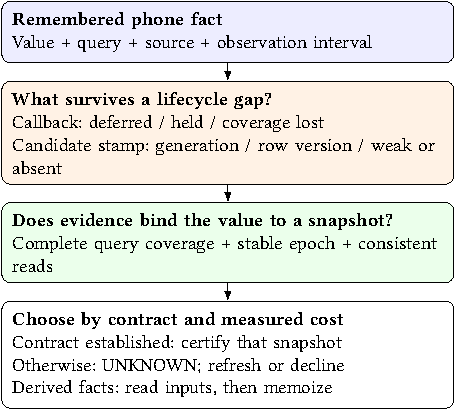
\includegraphics[width=\columnwidth]{figures/fig1-evidence-map.pdf}
\caption{The evidence map separates notification delivery, candidate stamps and snapshot certification. No branch certifies a later action automatically.}
\Description{Four linked boxes show a remembered fact, evidence surviving a lifecycle gap, the conditions for snapshot certification, and the choice between certification, UNKNOWN, refresh and memoization.}
\label{fig:overview}
\end{figure}

Mobile agents remember contacts, messages, photos and meetings across tasks. MobileGPT maintains app memory~\cite{lee2024mobilegpt}; broader memory systems persist facts for later reasoning~\cite{packer2023memgpt,chhikara2025mem0,rasmussen2025zep}. A remembered copy of phone state is a cache entry. Before using it, a client needs evidence that its query still has the same answer.

Android makes that evidence deployment-dependent. Processes can be killed, frozen or restarted~\cite{lebeck2020marvin,liang2020acclaim,android_freezer,android_doze}, and SMS, call-log and all-files access are restricted~\cite{play_smscalllog,play_allfiles}. Research agents often read through a host-side controller~\cite{rawles2025androidworld,zhang2025appagent,wang2024mobileagent}, whose on-device notification relay inherits Android's lifecycle and callback timing. We measure what such clients can infer for seven sources and four deployments, on Android~13 and 15 emulators and on rented Pixel~8 and Galaxy~S25 phones.

\paragraph{What the phones show.} Four results shape the design. (1) \emph{Stamps are candidates, not certificates.} Reading a value and then its version certified a changed value in \PhysRaceStale of \PhysRaceTrials races on the Pixel~8 and \PhysSamsungRaceStale of \PhysSamsungRaceTrials on the Galaxy~S25 (Tables~\ref{tab:phys-race} and~\ref{tab:phys-samsung}); a Contacts provider reset left the stamp unchanged in \PhysResetSameStamp Pixel~8 trials (\S\ref{sec:meas-gaps}). (2) \emph{The device decides the gap.} Pixel~8 units ran \PhysBuilds builds and \PhysFreezerOffTrialUnits had the cached-app freezer off by default; the Galaxy~S25 froze a cached client in \PhysSamsungFrozen attempts (Pixel~8: \PhysFreezerProbeFrozen); and its Contacts notifications carry a hidden no-delay flag, so a background client heard Contacts changes after \PhysSamsungBgMedian, against \PhysDeployBgMedian on the Pixel~8, while MediaStore stayed deferred (Table~\ref{tab:phys-samsung}). (3) \emph{Re-validation at the action boundary does not close the race:} on the Pixel~8, \PhysBndOverlapStale changes overlapping the check or the effect still produced stale effects (Table~\ref{tab:phys-boundary}). (4) \emph{Cheaper is not safer.} Through a host helper, batched optimistic stamp checks beat batched refresh only by re-reading fewer facts (from \PhysHostReadsStampMin to \PhysHostReadsStampMax against \PhysHostReadsRefresh; Table~\ref{tab:phys-host}); that is the policy of result (1), so we do not recommend it.

\paragraph{Gap classes.} A gap defers callbacks, holds them during freezing or loses observer coverage, and each class needs a different strategy: deferred or held callbacks leave event-only invalidation stale until delivery, while lost coverage makes persisted flags unsafe and requires refresh after restart. Timestamps are weaker evidence than versions, and file mtimes were coarse on the emulators but not on the Pixel~8.

\paragraph{Two policies.} \stamp is an optimistic diagnostic baseline that reads a value and then its stamp, so a write between those reads can label an old value with a new stamp. \sys instead requires a consistent observation, a complete validation interval and reset-safe evidence; stock adapters without that contract return \Unknown, and a cooperative transactional provider supplies positive controls.

\paragraph{Practical consequences.} Inside the client, direct provider refresh is faster than \stamp (\CostGl versus \CostLm\,ms per decision on the emulators, \PhysCostGl versus \PhysCostLm\,ms on the Pixel~8), and input memoization reduces model calls. A notification relay is cheaper still but inherits its helper's lifecycle. Because the gap class must be observed on the device, Table~\ref{tab:guidance} starts from a run-time check and then chooses by deployment, evidence and measured cost.

\paragraph{Contributions.} We provide (1) an Android source and deployment evidence map with lifecycle measurements on emulators and two rented phone models; (2) comparisons of notification, refresh, memoization and optimistic validation, with independent trial counts and matched host transport; and (3) a conditional consistency contract, device-executed counterexamples and a cooperative positive control. Version validation itself is established practice~\cite{gray1989leases,howard1988afs,rfc9110,rfc6578}. Our contribution is determining where its assumptions hold, fail or remain unestablished for this mobile workload.

\section{Background}
\label{sec:background}
\paragraph{Notifications and durable state.} \texttt{ContentObserver} callbacks require a live registered process~\cite{android_contentobserver}. ContentService immediately serves sufficiently important processes or writes marked \texttt{NOTIFY\_NO\_DELAY}; other callbacks wait its 10-second background delay~\cite{aosp_contentservice}. JobScheduler content-URI triggers survive process death but cannot persist across reboot~\cite{aosp_jobinfo}. Neither mechanism provides a replayable provider history. Counters, versions, timestamps and tombstones may supply that history if their coverage and reset contracts hold; direct reads instead obtain current query results.

\paragraph{Provider and lifecycle boundaries.} Contacts and Calendar sync metadata belongs to the account's sync adapter, which clears dirty/deleted flags after synchronization~\cite{android_syncadapter}. A third-party reader cannot assume those flags constitute its own change log. Android exposes MediaStore generation evidence, while iOS Contacts and Photos expose reader-side history~\cite{apple_cnchangehistory,apple_phpersistent}.

Cached processes may be killed or frozen~\cite{lebeck2020marvin,liang2020acclaim,android_freezer}. One-way observer calls wait during freezing. Force-stop cancels jobs and alarms; permission revocation kills the process; unregistration removes callback coverage. Doze and standby buckets constrain background execution~\cite{android_doze}; our tested schedules show no additional observer delay beyond background deferral. A new process identity or \texttt{ApplicationExitInfo} identifies absence, not intervening provider changes~\cite{android_exitinfo}.

\paragraph{Scope.} We study benign staleness with recorded sources and queries. Lifecycle probes use deterministic scripts; derived-fact and resumed-task experiments invoke local LLMs. The target is external-state memory, not planning quality. Screen-only facts without a supported query binding remain \Unknown.

\section{Measurement: What Android Keeps and What Gaps Do}
\label{sec:measurement}

This section reports the source and lifecycle campaigns on emulators: Android~13 (API~33) on two AVDs and Android~15 (API~35) on a third (\S\ref{sec:eval-setup}). The closing sentences of a subsection repeat its campaign on the rented phones of \S\ref{sec:phys-setup}. Mutations come from a separate app through public APIs (\S\ref{sec:impl}). Candidate stamps are not complete certificates; the consistent contract and new tests appear in \S\ref{sec:design} and \S\ref{sec:checks}. Table~\ref{tab:phone-results} puts the phone results next to the emulators.

\begin{table}[t]
\centering\mtab
\caption{Phone results next to the emulators (details in Tables~\ref{tab:phys-deploy}, \ref{tab:phys-race}, \ref{tab:phys-boundary} and~\ref{tab:phys-samsung}). Callbacks: Contacts medians unless noted. Emulator column: background and FGS callbacks from the Android~13 verified-state runs (Table~\ref{tab:deploy}); MediaStore from all provider sources of the Android~13 source probes; no-delay flag, frozen trials, reset and race pooled over Android~13 and~15; check-to-effect from the emulator boundary experiment (Table~\ref{tab:boundary}). Freezer off: units behind reported trials. Frozen: cached client with the freezer on (S25: watched for at least \PhysSamsungFreezeWindowS\,s); emulators: frozen trials. Race: stale \Fresh after updates and inserts to sources whose stamp certifies, on a seeded schedule, so counterexamples rather than rates. n/a: not run.}
\label{tab:phone-results}
\begin{tabular}{lrrr}\toprule
\mhead Result & Pixel~8 & Galaxy~S25 & Emulator\\\midrule
Background callback & \PhysDeployBgMedian & \PhysSamsungBgMedian & \FollowABg\\
Background, MediaStore & \PhysDeployMediaBgMedian & \PhysSamsungMediaBgMedian & \ProvLatA\,s\\
FGS callback & \PhysDeployFgMedian & \PhysSamsungFgMedian & \FollowAFg\\
No-delay flag & \PhysDeployNoDelay & \PhysSamsungNoDelay & \PhysEmuNoDelay\\
Freezer off by default & \PhysFreezerOffTrialUnits & \PhysSamsungFreezerOffTrialUnits & n/a\\
Cached client frozen & \PhysFreezerProbeFrozen & \PhysSamsungFrozen & \PhysEmuFrozen\\
Check-to-effect & \PhysCteMs\,ms & n/a & \CteMs\,ms\\
Contacts reset keeps stamp & \PhysResetSameStamp & n/a & \PhysResetEmuSameStamp\\
Race: value, then version & \PhysRaceStampedStale & \PhysSamsungRaceStampedStale & \PhysRaceEmuStampedStale\\
\bottomrule\end{tabular}
\end{table}

\subsection{Which sources keep durable change evidence?}
\label{sec:meas-coverage}

% AUTO-GENERATED by artifact/scripts/render.py; do not edit
\begin{table}[t]
\centering
\caption{Durable change evidence on Android~13 (E1): trials in which a candidate moved after one mutation of each kind by another app; ``None'' = source untouched. $\downarrow$: moved downward in some trials. All probed candidates and the Android~15 replication are in Table~\ref{tab:allcands}.}
\label{tab:coverage}
\mtab\scriptsize
\setlength{\tabcolsep}{2.4pt}
\begin{tabular}{llrrrr}
\toprule
\mhead Source & Candidate & Insert & Update & Delete & None \\
\midrule
Contacts & max last-updated ts & 25/25 & 36/36 & 5/24$^{\downarrow}$ & 0/20 \\
 & max deleted-contact ts & 0/25 & 0/36 & 24/24 & 0/20 \\
 & sum RawContacts \texttt{VERSION} & 25/25 & 36/36 & 24/24$^{\downarrow}$ & 0/20 \\
\addlinespace[1pt]
Call log & max \texttt{LAST\_MODIFIED} & 33/33 & 30/30 & 22/22$^{\downarrow}$ & 0/20 \\
 & max \texttt{\_id} & 33/33 & 0/30 & 22/22$^{\downarrow}$ & 0/20 \\
\addlinespace[1pt]
SMS & max \texttt{\_id} & 29/29 & 0/24 & 27/29$^{\downarrow}$ & 0/23 \\
 & max \texttt{date} & 29/29 & 0/24 & 27/29$^{\downarrow}$ & 0/23 \\
 & row count & 29/29 & 0/24 & 29/29$^{\downarrow}$ & 0/23 \\
\addlinespace[1pt]
MediaStore & \texttt{getGeneration} & 29/29 & 23/23 & 27/27 & 16/26 \\
 & max \texttt{generation\_modified} & 29/29 & 23/23 & 13/27$^{\downarrow}$ & 0/26 \\
\addlinespace[1pt]
Calendar & max \texttt{\_id} & 21/21 & 0/37 & 0/16 & 0/31 \\
 & sum \texttt{dirty} & 21/21 & 0/37 & 16/16$^{\downarrow}$ & 0/31 \\
\addlinespace[1pt]
Shared files & directory mtime & 17/17 & 0/34 & 27/27 & 0/27 \\
 & max file mtime & 17/17 & 34/34 & 1/27$^{\downarrow}$ & 0/27 \\
\midrule
\multicolumn{2}{l}{\stamp Contacts adapter (VERSION map, E2)} & 82/82 & 62/62 & 51/51 & 0/192 \\
\multicolumn{2}{l}{SMS, calendar events, Settings: none found} & \multicolumn{4}{c}{$\Rightarrow$ \Unknown} \\
\bottomrule
\end{tabular}
\end{table}


In each of \EOneTrials Android~13 trials (\EOneBgTrials with the client in the background, \EOneFgTrials in the foreground), the client probed every candidate. The mutator then applied one random mutation, or none, to each of seven sources, and after 13\,s the client probed again. Table~\ref{tab:coverage} reports the candidates behind each design decision. Table~\ref{tab:allcands} (appendix) lists all of them and the \EOneApiTrials-trial Android~15 replication.

\textbf{Counter and row-version candidates.} MediaStore's volume generation~\cite{android_mediastore} moved on every insert, rename and delete, sometimes also in unchanged trials; the maximum row generation fell after deletes. Contacts RawContacts versions detected all tested mutation types without a wall clock. \stamp checks the complete raw-contact $(id,contact,version,deleted)$ map; its timestamp ablation is vulnerable to clock rollback (\S\ref{sec:eval-pitfalls}). Neither candidate alone supplies the snapshot/reset contract of \S\ref{sec:design}. Table~\ref{tab:phys-coverage} repeats this probe on the phone (\PhysCoverageTrials trials) with the same pattern.

\textbf{Weak or absent evidence.} Call-log \texttt{LAST\_MODIFIED} timestamps detected tested edits; deletion requires row-existence checks. SMS and calendar edits changed no candidate stamp, local calendar dirty flags remained set, and SMS identifiers can recur. Settings' generation tracker is hidden, though ordinary reads use an in-process cache. App-written files under \texttt{Documents/} appeared as pending MediaStore rows whose generations did not advance through appends; one-second mtimes are also insufficient for strict certification.

\paragraph{Live notifications to background processes are deferred.} Table~\ref{tab:latency} (appendix) gives the source-probe callback delays. Android~13's background median is \ProvLatA\,s, consistent with ContentService's 10\,s \path{BACKGROUND_OBSERVER_DELAY}~\cite{aosp_contentservice}; foreground callbacks take \FgLatMs\,ms and FileObserver takes \FileLatMs\,ms. The mixed-state Android~15 source-probe median is \ProvLatB\,s. The separate no-gap policy campaign reports \FclApiNone\,s (Table~\ref{tab:gaps}). Both campaigns are mixed-state measurements confounded by shortened freezer settings; \S\ref{sec:checks} isolates unfrozen and frozen processes, and Figure~\ref{fig:age} does not pool the Android~15 curve. Source-probe samples spanning host sleep (\LatDropped above 60\,s) are excluded. On the Pixel~8, the same deferral gives a background Contacts median of \PhysDeployBgMedian (Table~\ref{tab:phys-deploy}).\ifPhysSamsung{} On a Galaxy~S25, MediaStore callbacks were deferred the same way (\PhysSamsungMediaBgMedian), but Contacts callbacks reached the cached, unfrozen client in \PhysSamsungBgMedian: the first Contacts callback of every trial, in all three deployments, carried the hidden \texttt{NOTIFY\_NO\_DELAY} flag (\PhysSamsungNoDelay), which exempts a notification from the deferral (Pixel~8: \PhysDeployNoDelay; Table~\ref{tab:phys-samsung}).\fi

\subsection{What does each gap do?}
\label{sec:meas-gaps}

% AUTO-GENERATED by artifact/scripts/render.py -- do not edit
\begin{table*}[t]
\centering
\caption{What each gap does to a live or restarted client (E2). First callback: median / max delay from a provider mutation to its first \texttt{ContentObserver} callback. Notified: share of changed provider sources with a callback by the early (+2\,s) and late (+14\,s) decision. Trigger: the JobScheduler content trigger (its own package, same gap) fired. Exit: new \texttt{ApplicationExitInfo} records.}
\label{tab:gaps}
\mtab\scriptsize
\begin{tabular}{lrrrrrrl}
\toprule
\mhead Gap & Trials & Survived\,\% & First callback (s) & Notified early\,\% & Notified late\,\% & Trigger\,\% & Exit record \\
\midrule
\mgroup{8}{Android 13, background client}
No gap (control) & 25 & 100 & 10.0 / 10.0 & 72 & 100 & 100 & 0/25 \\
Cached-app freezer & 29 & 100 & 18.3 / 31.7 & 91 & 100 & 100 & 0/29 \\
Doze (deep idle) & 25 & 100 & 10.0 / 10.0 & 88 & 100 & 100 & 0/25 \\
Restricted bucket & 25 & 100 & 10.0 / 10.1 & 72 & 100 & 100 & 0/25 \\
Freezer, default debounce & 5 & 100 & 62.5 / 62.9 & 94 & 100 & 100 & 0/5 \\
Doze, stepped (idle not held) & 5 & 100 & 10.0 / 10.1 & 100 & 100 & 100 & 0/5 \\
Doze, verified deep idle & 10 & 100 & 10.0 / 10.1 & 100 & 100 & 100 & 0/10 \\
Observer unregistered & 25 & 100 & -- & 0 & 0 & 100 & 0/25 \\
Killed (\texttt{am kill}) & 25 & 0 & -- & 0 & 0 & 100 & 25/25 {\scriptsize USER\_REQUESTED} \\
Force-stop & 25 & 0 & -- & 0 & 0 & 0 & 25/25 {\scriptsize USER\_REQUESTED} \\
Permission revoked & 25 & 0 & -- & 0 & 0 & 100 & 25/25 {\scriptsize PERMISSION\_CHANGE} \\
Reboot & 25 & 0 & 34.1 / 51.1 & 0 & 5 & 5 & 0/25 \\
\mgroup{8}{Android 13, foreground-service client}
No gap (control) & 15 & 100 & 7\,ms / 0.0 & 100 & 100 & 100 & 0/15 \\
Doze (deep idle) & 15 & 100 & 7\,ms / 0.0 & 100 & 100 & 100 & 0/15 \\
Observer unregistered & 15 & 100 & -- & 0 & 0 & 100 & 0/15 \\
Killed (\texttt{SIGKILL}) & 15 & 0 & -- & 0 & 0 & 100 & 15/15 {\scriptsize SIGNALED} \\
Force-stop & 15 & 0 & -- & 0 & 0 & 0 & 15/15 {\scriptsize USER\_REQUESTED} \\
Reboot & 15 & 0 & 15\,ms / 15.3 & 42 & 44 & 11 & 0/15 \\
\mgroup{8}{Android 15, background client; mixed freezer state}
No gap (control) & 12 & 100 & 18.0 / 31.6 & 61 & 100 & 100 & 0/12 \\
Cached-app freezer & 12 & 100 & 17.7 / 25.8 & 21 & 95 & 100 & 0/12 \\
Observer unregistered & 12 & 100 & -- & 0 & 0 & 100 & 0/12 \\
Killed (\texttt{am kill}) & 12 & 0 & -- & 0 & 0 & 100 & 12/12 {\scriptsize USER\_REQUESTED} \\
\bottomrule
\end{tabular}
\end{table*}


Table~\ref{tab:gaps} separates the gaps by their effect on the process and on notifications. Each trial holds the gap from 0 to 30\,s after mutating, so a change is from 2 to 32\,s old at the early decision (protocol in \S\ref{sec:eval-setup}). The first-callback column gives the delay from each provider mutation to its first callback. Three classes emerge.

\emph{Deferred only} (no gap, Doze, restricted bucket). The process survived every trial, and every callback came after the same ContentService deferral as without a gap: median \FclNone\,s with no gap, \FclDozeidle\,s in deep Doze and \FclBucket\,s in the restricted bucket (maxima \FclMaxNone, \FclMaxDozeidle and \FclMaxBucket\,s). These trials show no additional delay attributable to Doze or the bucket. The stepped long-Doze gap gives the same \FclLongdoze\,s, and so does a 10-minute gap in which deep idle was verified at both mutation batches (\FclLongdozeTwo\,s; \S\ref{sec:eval-validity}).

\emph{Held until thaw} (cached-app freezer). Callbacks to a frozen process wait until it thaws; the first-callback delay grows with the hold (median \FclFreeze\,s for holds from 0 to 30\,s). Whether long holds lose callbacks is tested in \S\ref{sec:meas-frozen}. On the phone, where Doze is also forced, median first callbacks are \PhysGapNoneFcl, \PhysGapDozeFcl and \PhysGapBucketFcl\,s with no gap, deep Doze and the bucket, as on the emulators, and \PhysGapFreezeFcl\,s with the freezer (\PhysGapTrials trials; Table~\ref{tab:phys-gaps}).\ifPhysSamsung{} On a Galaxy~S25 the cached client never froze within \PhysSamsungFreezeWindowS\,s with the freezer on (\PhysSamsungFrozen attempts), so no callback was held there in that window; longer windows and any vendor-specific freezing were not tested.\fi

\emph{Lost} (unregistration, kill, force-stop, revocation, reboot). Notifications sent while no observer is registered are never delivered and never replayed. Kill, force-stop and revocation leave an \texttt{ApplicationExitInfo} record, and reboot leaves none. A record tells the app that it was absent, not what changed.

The JobScheduler trigger lives in its own package, which is subjected to the same gap, as if the trigger belonged to the agent. It survived process death, but not force-stop or reboot. An FGS client is never cached or frozen (oom\_adj from \OomFgMin to \OomFgMax vs.\ from \OomBgMin to \OomBgMax in the background), and its callbacks arrived in \FgLatMs\,ms. \texttt{am kill} targets only background processes, so the FGS client's kill gap uses \texttt{SIGKILL}; in every background kill trial \texttt{am kill} did end the process (\AmkillAlive survived).
Durable evidence can itself be reset. After \RebootEmpty of \RebootN reboots the Contacts database came back empty, rows and tombstone log alike. MediaStore's version string never changed across a reboot (\RebootMediaVer changes).\ifPhysReset{} On the phone, a Contacts provider reset followed by the same fixtures left the Contacts stamp unchanged in \PhysResetSameStamp trials (emulators: \PhysResetEmuSameStamp); strict \sys returned \Unknown in \PhysResetUnknown.\fi

\subsection{Are callbacks to a frozen process lost?}
\label{sec:meas-frozen}

% AUTO-GENERATED by artifact/scripts/render.py; do not edit
\begin{table}[t]
\centering
\caption{Long frozen holds: the client is frozen and stays in the background while another app changes a random source every 3\,s for at least the stated time after the first change; decisions at +2, +14 and +120\,s after the gap. Killed: the frozen process was killed during the hold. Lost sources and unseen last changes are counted over the trials that stayed frozen: mutated sources with no callback by +120\,s, and sources whose last change had no later callback. Last row: changed uses missed by restart-aware event-only at +2/+14/+120\,s.}
\label{tab:frozen}
\mtab
\begin{tabular}{lrr}
\toprule
\mhead Metric & Android 13 & Android 15 \\
\midrule
Trials & 20 & 20 \\
Stayed frozen & 19 & 20 \\
Killed & 1 & 0 \\
Changes & 3859 & 3868 \\
Hold $\geq$ (min) & 10.0 & 10.0 \\
Lost sources & 0/133 & 0/140 \\
Unseen last & 0/133 & 0/140 \\
Callbacks & 5294 & 8182 \\
Restart-aware miss & 54/0/0 & 107/0/0 \\
\bottomrule
\end{tabular}
\end{table}


A long-hold campaign holds the client frozen for ten minutes, with mutations every three seconds and verified frozen-state samples. Table~\ref{tab:frozen} reports the independent holds and their outcomes. In the \NineStayedA Android~13 and \NineStayedB Android~15 holds that stayed frozen, all \NineSrcMutA and \NineSrcMutB mutated sources had a callback after their last change. This is source invalidation coverage, not lossless delivery of individual callbacks. Restart-aware event-only missed \NineEvrEarlyA and \NineEvrEarlyB changed uses at +2 seconds, and \NineEvrLateA and \NineEvrLateB at +14 seconds. Re-freezing after thaw complicates the Android~15 timing interpretation. ActivityManager killed the process in \NineDiedA and \NineDiedB holds; a freeze cannot be assumed to end in thaw. On the phone, \PhysFrozenStayed of \PhysFrozenHolds holds stayed frozen, \PhysFrozenLastUnseen sources had no callback after their last change and \PhysFrozenKilled holds were killed, as on the emulators (Table~\ref{tab:phys-frozen}).

\subsection{Which gaps apply to which deployment?}
\label{sec:meas-deploy}

\begin{table*}[t]
\centering\mtab
\caption{Verified-state Contacts callbacks: median and range, with valid/attempted trials. Frozen trials hold 14 seconds after mutation; root-side reads do not wake the client. Callback counts are before/after foreground thaw. Each source change is one independent trial; this is not a handset replication.}
\label{tab:deploy}
\begin{tabular}{lrllrr}\toprule
\mhead Deployment & Trials & Median & Range & Before & After\\\midrule
\mgroup{6}{Android 13}
Bound assistant (target 35) & 20/20 & 5\,ms & [4\,ms, 10\,ms] & 20/20 & 20/20\\
Background, frozen & 20/20 & held & n/a & 0/20 & 20/20\\
Background, unfrozen & 20/20 & 10.0\,s & [10.007\,s, 10.037\,s] & 20/20 & 20/20\\
Foreground service & 20/20 & 8\,ms & [5\,ms, 11\,ms] & 20/20 & 20/20\\
Persistent system app & 20/20 & 22\,ms & [12\,ms, 63\,ms] & 20/20 & 20/20\\
\mgroup{6}{Android 15}
Bound assistant (target 35) & 20/20 & 6\,ms & [4\,ms, 10\,ms] & 20/20 & 20/20\\
Background, frozen & 20/20 & held & n/a & 0/20 & 20/20\\
Background, unfrozen & 20/20 & 10.0\,s & [10.006\,s, 10.027\,s] & 20/20 & 20/20\\
Foreground service & 20/20 & 6\,ms & [5\,ms, 10\,ms] & 20/20 & 20/20\\
\bottomrule\end{tabular}
\end{table*}


Table~\ref{tab:deploy} expands the callback experiment to 20 Contacts changes per platform and deployment, with frozen state sampled before and during every hold. The assistant targets API~35 and must have a live \path{VoiceInteractionService} binding. Background and FGS fixtures target API~33. Unlike the latency experiment, separate lifecycle probes test kill and force-stop: the bound assistant and FGS survive \texttt{am kill}; force-stop ends them, but the Android~15 assistant restarts. The Android~13 persistent-system cohort also has 20 Contacts changes: a boot-installed privileged app runs at oom adjustment $-800$, with callback median \FollowAPersist (range in Table~\ref{tab:deploy}). Its permissions are granted before restarting the persistent process and registering observers. The separate lifecycle probes found neither kill nor force-stop ended this privileged process; a call-log observer required a hard-restricted permission allowlist.


Epoch-breaking gaps require restart repair, but prompt in-epoch callbacks still leave a write-to-delivery interval (Observation~\ref{thm:indist}). On the phone, Contacts medians are \PhysDeployFgMedian with an FGS and \PhysDeployAssistMedian for the assistant, an order of magnitude above the emulators' yet tens of milliseconds, and as on the emulators \PhysDeployFrozenBeforeThaw frozen trials had a callback before thaw; MediaStore medians are \PhysDeployMediaBgMedian in the background and \PhysDeployMediaFgMedian{} with an FGS\ifPhysCalllog, call-log medians \PhysDeployCalllogBgMedian and \PhysDeployCalllogFgMedian{}\fi{} (\PhysDeployTrials trials; Table~\ref{tab:phys-deploy})\ifPhysCalllog\else; the call log is not tested on the phone\fi.

\subsection{How much agent-relevant state has evidence?}
\label{sec:meas-aw}



The source census maps \AwTasks AndroidWorld tasks~\cite{rawles2025androidworld} through app names to stores (Table~\ref{tab:aw}, appendix). A name-based rule selects \AwRead tasks that might read pre-existing state, of which \AwReadWm involve only stores with candidate stamps. These are app/name classifications, not validated facts or strict certificates. Private-state access by the benchmark's privileged validator is also distinct from ordinary app access. A nine-query inspection in Appendix~\ref{app:stamp-based} examines these differences directly.

\section{Consistent Evidence and Conservative Validation}
\label{sec:design}
A certificate must bind a value to the evidence that certifies it. A remembered fact is stored with its source, query/projection, value, support, adapter contract, provider epoch, evidence version and read interval. Entries without this schema, exceptions, missing evidence and unsupported contracts are \Unknown, not successful empty reads. Notifications are invalidation hints; silence is not a certificate.

\paragraph{Observation and re-anchoring.} Two protocols are possible. A cooperative provider can return value, support, epoch and sequence from one transaction. Alternatively, a reader obtains complete evidence $E_0$, executes the query and its support reads, and obtains $E_1$. Equality is sufficient only if the adapter establishes that every relevant committed change alters the evidence, the provider epoch cannot silently recur, and all reads obey the stated consistency model. Neither zero-miss trials nor equality of timestamps, repeated values or digests establishes those premises. A mismatching pair restarts the entire operation, for at most three attempts; exhaustion returns \Unknown. Refresh and re-anchoring use the same protocol, never a value from one attempt and a version from another. Algorithm~\ref{alg:validate} in Appendix~\ref{app:proofs} states the procedure for one source.

\paragraph{Validation's certified instant.} The protocol brackets the complete sequence of watermark, support, delta and query reads. A successful bracket certifies the query snapshot inside that stable interval. The log records its in-transaction timestamp and the enclosing read interval. \Changed denotes a witnessed value change; reset epochs and incomplete evidence yield \Unknown. A provider version change does not by itself prove that a particular fact changed.

\paragraph{Stock adapters.} We inspect complete Contacts version maps, MediaStore identity/generation and call-log row contents alongside the optimistic stamps. The stock workload uses joins, query membership and sometimes several cursors. The public Contacts columns give per-row versions and timestamps but no provider-wide sequence or epoch across the raw-contact, data and aggregate tables a query joins. Reading a row's value and version in one cursor would therefore not cover these paths: membership, deletions and joined rows need further queries, and a provider wiped and refilled reproduced its versions (\S\ref{sec:meas-gaps}). For MediaStore, a row's \texttt{generation\_modified} read with its stable ID covers at most that one row: it misses rows entering or leaving the query and deleted rows, and read apart from the value it was fooled in \PhysRaceMediaStampedStale race trials. Lacking an atomic epoch and query contract for these paths, strict stock certification stays disabled; direct refresh remains, with its read interval recorded.

\paragraph{Cooperative reference.} A separate Android provider process stores one keyed row and an epoch/sequence pair in SQLite. Every supported mutation and deletion increments the sequence in its transaction; managed reset or restore rotates the epoch in the same transaction. All writers must use this API. Because the query snapshot is already atomic, a stable bracket adds only retries. The reference is thus a one-row positive control: its \RevReference trials check that client and oracle follow the procedure through deletion, identifier reuse, reset and injected writes (guards in Appendix~\ref{app:proofs}). Its scope is one keyed row, one writer API and one provider process; multi-row queries, joins, sync adapters and stock providers lie outside it, and its bracket cost does not price a large provider.

\paragraph{Several sources.} Separately refreshed or certified inputs are each current at their own instant, and Android offers no joint snapshot across providers. Tasks correct when each input was current at its read, such as the drafts in \S\ref{sec:agent-tasks}, tolerate this; tasks that relate sources remain \Unknown. An effect that must not act on a changed input, such as calling a just-validated number, needs a provider-side conditional effect: re-validating just before it shortens, but no re-validation, fixed wait or fast callback delivery closes, the interval in which an overlapping write changes the fact (\S\ref{sec:eval-boundary}).

\section{Guarantees and Limits}
\label{sec:theory}
Let $q(\sigma_t)$ be a fact's value at time $t$. An observation certificate binds a value to an actual query snapshot. Validation must establish a later snapshot or stable interval for that same query, rather than merely record a subsequently read watermark.

\begin{assumption}[Consistent evidence]\label{as:evidence}
\begin{enumerate}[nosep,leftmargin=*]
\item Every relevant commit changes a non-repeating sequence within its epoch.
\item Supported reset/restore changes the epoch, without silent reuse.
\item Value and support reads are snapshots, or are bracketed by complete evidence whose equality establishes an unchanged interval.
\item Validation includes every support, delta and membership read.
\item Failures withdraw certification.
\end{enumerate}
\end{assumption}

\begin{theorem}[Conditional snapshot freshness]\label{thm:sound}
Under Assumption~\ref{as:evidence}, a successful observation records its query's value at a certified instant. A validation that returns \Fresh certifies equality of that stored value and the query at its own certified instant. It does not certify response receipt, an independent source, or a later effect.
\end{theorem}
The proof is direct: an atomic snapshot binds value and sequence; for a successful bracket, non-repeating complete evidence excludes intervening relevant commits. The query belongs to that interval, and comparison therefore refers to a consistent state. A mismatched epoch, failed read or exhausted retry produces no certificate. These are implementation obligations, not properties established by a finite number of zero-miss trials. In particular, a nondecreasing clock is weaker than a strictly changing sequence, and a digest of row versions does not supply a database incarnation identifier.

\begin{theorem}[Notification silence]\label{thm:indist}
If a relevant write can commit before its notification is delivered, a reader using only its prior state, delivered notifications and lifecycle records cannot distinguish that execution from an unchanged source before delivery. It must read establishing evidence, refresh, or decline to certify.
\end{theorem}
This includes short in-epoch delivery delays, not just process-ending gaps. Refresh-on-restart addresses lost coverage under the tested post-gap schedules. Waiting for old callbacks is sufficient only with separately established writer quiescence and delivery completion; a fixed duration does not establish either premise.

\begin{proposition}[Cost accounting]\label{prop:cost}
A validated bracket pays for both evidence reads, all support/delta/query reads, failed attempts and fallback refreshes. A host additionally pays transport, serialization and helper residency. An unsupported source incurs refresh cost if the client requires a usable value. Input memoization pays for current inputs and recomputes only changed derived outputs.
\end{proposition}
The one-watermark \stamp cost does not price \sys; each result identifies the measured policy. Neither the theorem nor the cost accounting implies that validation is faster than refresh.

\section{Implementation}
\label{sec:impl}
The main client targets API~33; the bound-assistant and FGS compatibility fixtures target 35. The client registers observers, persists memory by atomic rename and evaluates policies before the comparison read. Mutations use public provider/file APIs with test-granted permissions.

The client implements \stamp and strict \sys with schema-v4 certificates, a loopback helper and a separate-process transactional SQLite provider. Reference writes/reset obey its managed contract. Seeded drivers record process state, APK/source hashes, failures and exclusions. A separate Python oracle checks certificates without invoking Java verdict logic. The artifact retains cohort-specific sources and distinguishes summed-call costs from directly measured task execution. It also holds every phone run's raw per-trial logs (unit, build and run identifiers on each record), the run log and exclusion list, and the scripts that regenerate every table and number in this paper from them.

% Physical-phone setup (task A4b, AWS Device Farm). Details live in PHYS-PROTOCOL.md; numbers come from generated/physical_macros.tex.
\paragraph{Physical phone.}\label{sec:phys-setup} Physical runs use one \PhysDevice (\PhysAndroid, build \PhysFingerprint, root: \PhysRooted) rented on AWS Device Farm. A run lasts at most 150 minutes on a freshly reset phone, so each run installs the apps, grants permissions and writes synthetic fixtures itself; the Python drivers run on the Device Farm Linux host and reach the phone over adb. Runs may land on different units of the model, so every trial records its unit (distinct units: \PhysInstances). The phone stays on the charger: Doze is forced with \texttt{dumpsys battery unplug} and \texttt{deviceidle force-idle deep}, and we measure neither battery drain nor unplugged use. Without root, the drivers use \texttt{run-as}, the cgroup files and \texttt{dumpsys activity} for app files, kills and frozen state. Clock rollback, Contacts reset\ifPhysSms\else, SMS\fi\ifPhysCalllog\else, the call log, the action-boundary test (its effect is a call-log row)\fi\ifPhysReboot\else, the reboot gap\fi{} and the persistent system app keep emulator results. \texttt{PHYS-PROTOCOL.md} in the artifact lists the commands and exclusions.

\section{Evaluation}
\label{sec:eval}

\subsection{Optimistic Campaign: Setup}
\label{sec:eval-setup}

\paragraph{Platforms, workload and gaps.} These campaigns ran on emulators: two Android~13 AVDs and one Android~15 AVD on one host (images, builds and freezer settings in Appendix~\ref{app:stamp-based}). Sixteen provider/file facts and three derived facts cover contacts, SMS, calls, media, calendars, settings and files (Table~\ref{tab:facts}); a separate app inserts, edits or deletes records. Each trial observes after setup, injects and verifies a gap, mutates sources with probability 0.5, and decides at +2 and +14 seconds after a hold of 0 to 30 seconds. Process-ending gaps relaunch the client. The optimistic sample contains \ETwoBg background and \ETwoFg FGS trials on Android~13 and \ETwoApi on Android~15; schedules and exclusions are in the appendix.

\paragraph{Implementation scope.} The measurements below describe the retained optimistic client (non-atomic anchoring, weak timestamp adapters) under staged post-observation schedules; the conservative client is evaluated in \S\ref{sec:checks}.

\paragraph{Policies.} Event-only (persisted source-level flags); restart-aware event-only (refresh everything after an epoch break); Tether-style (dependency propagation from delivered events, without durable source stamps); +OS trigger (event-only plus the JobScheduler trigger); \stamp; \stamp-TS; \stamp-epoch; global refresh; for derived facts, input memoization. All in-app policies are evaluated on the same decision, before the decision-time comparison read. The trigger is evaluated from its log.

\paragraph{Metrics and statistics.} A fact use is \emph{changed} if the remembered value differs from the provider value read at decision time. A policy \emph{misses} a changed use it does not refresh, which is a stale critical decision. Per-use rates count derived facts, which are deterministic functions of base facts. Table~\ref{tab:trial} therefore also gives trial-level rates (trials with at least one stale decision), the unit of independent replication. Proportions carry Wilson and medians bootstrap 95\% intervals (2{,}000 resamples, fixed seed). Most cells are 0\% or 100\%, so trial-level tests appear only where outcomes vary (Table~\ref{tab:sig}).

\subsection{RQ1: Which designs avoid stale decisions?}
\label{sec:eval-rq1}

% AUTO-GENERATED by artifact/scripts/render.py -- do not edit
\begin{table*}[t]
\centering
\caption{Missed changes (\% of changed fact uses) by gap group, early (E, +2\,s) and late (L, +14\,s) decision. For a background client the three groups are the deferred, held-until-thaw and lost classes of \S\ref{sec:meas-gaps}. Per-gap rows, Android~15 and trial-level counts are in Tables~\ref{tab:policy} and~\ref{tab:trial}.}
\label{tab:summary}
\mtab
\begin{tabular}{lrw{c}{1.7em}w{c}{1.7em}w{c}{1.7em}w{c}{1.7em}w{c}{1.7em}w{c}{1.7em}w{c}{1.7em}w{c}{1.7em}w{c}{1.7em}w{c}{1.7em}}
\toprule
\mhead Gap class & Trials & \multicolumn{2}{c}{\begin{tabular}[b]{@{}c@{}}Event-\\only\end{tabular}} & \multicolumn{2}{c}{\begin{tabular}[b]{@{}c@{}}Restart-\\aware\end{tabular}} & \multicolumn{2}{c}{\begin{tabular}[b]{@{}c@{}}+OS\\trigger\end{tabular}} & \multicolumn{2}{c}{\begin{tabular}[b]{@{}c@{}}\textsc{Stamp-}\\\textsc{Check}\end{tabular}} & \multicolumn{2}{c}{\begin{tabular}[b]{@{}c@{}}Global\end{tabular}} \\ \mhead & & E & L & E & L & E & L & E & L & E & L \\
\midrule
\mgroup{12}{Android 13, background client}
No gap, Doze, bucket & 90 & \mbad{15} & 0 & \mbad{15} & 0 & \mbad{2} & 0 & 0 & 0 & 0 & 0 \\
Freezer & 34 & \mbad{9} & 0 & \mbad{9} & 0 & 0 & 0 & 0 & 0 & 0 & 0 \\
Unregister, kill, force-stop, revoke, reboot & 125 & \mbad{99} & \mbad{98} & 0 & 0 & \mbad{45} & \mbad{43} & 0 & 0 & 0 & 0 \\
\mgroup{12}{Android 13, foreground-service client}
No gap, Doze & 30 & 0 & 0 & 0 & 0 & 0 & 0 & 0 & 0 & 0 & 0 \\
Unregister, SIGKILL, force-stop, reboot & 60 & \mbad{90} & \mbad{90} & 0 & 0 & \mbad{48} & \mbad{47} & 0 & 0 & 0 & 0 \\
\bottomrule
\end{tabular}
\end{table*}

% AUTO-GENERATED by artifact/scripts/render.py; do not edit
\begin{figure}[t]
\centering
\begin{tikzpicture}
\begin{axis}[matured, width=\columnwidth, height=3.7cm, xmin=0, xmax=34, ymin=-3, ymax=103, xlabel={Age of the change at the decision (s)},
  ylabel={Missed changes (\%)},
  extra x ticks={10}, extra x tick labels={}, extra x tick style={grid=major, grid style={dashed,mSlate!60}},
  legend style={at={(0.98,0.62)}, anchor=east}]
\addplot[mBrick,mark=triangle*,mark size=1.8pt] coordinates {(2.0,83.3) (6.0,85.0) (9.0,88.9) (11.0,0.0) (14.0,0.0) (20.0,0.4) (32.0,0.0)};
\addlegendentry{Event-only, bg, Android 13}
\addplot[mNavy,mark=square*,mark size=1.4pt] coordinates {(2.0,0.0) (6.0,0.0) (9.0,0.0) (11.0,0.0) (14.0,0.0) (20.0,0.0) (32.0,0.0)};
\addlegendentry{Event-only, FGS, Android 13}
\addplot[mTeal,mark=*,mark size=1.4pt] coordinates {(2.0,0.0) (6.0,0.0) (9.0,0.0) (11.0,0.0) (14.0,0.0) (20.0,0.0) (32.0,0.0)};
\addlegendentry{\stamp, all}
\end{axis}
\end{tikzpicture}
\caption{Android~13 in-epoch gaps (no gap, freezer, Doze, bucket), base facts, both decisions: event-only misses concentrate among recent changes; none occur in the tested foreground-service schedules. Restart-aware equals event-only here (no epoch break).}
\Description{Missed-change rates by change age for Android 13 event-only background and foreground-service clients and the optimistic StampCheck probe. Recent changes dominate background misses in the staged schedules.}
\label{fig:age}
\end{figure}


Table~\ref{tab:summary} groups the gaps by the class of \S\ref{sec:meas-gaps}; per-gap rows are in Table~\ref{tab:policy} and trial-level rates in Tables~\ref{tab:checks-trials} and~\ref{tab:trial}.

\paragraph{Lost observer coverage makes persisted flags unsafe.} Across kill, force-stop, revocation, unregistration and reboot (background client, late decision), event-only missed \DeathEvK of \DeathChanged changed uses (\DeathEv). A dead or detached listener never hears the change, and our event-only memory trusts its persisted flags after a restart. The restart-aware variant missed \DeathEvrK: it refreshes every fact after an epoch break, \MeanEvrRefDeath of 16 per decision against \stamp's \MeanLmRefDeath. The OS trigger fires through a kill but is cancelled by force-stop and cannot outlive a reboot. \stamp missed \DeathLmK. In the FGS reboot gap event-only missed only part of the changes, because half of each trial's changes were made before the reboot, and the FGS client heard those at once; the background client's deferral outlasted the time to the reboot.

\paragraph{Delivery delay matters within an epoch.} Restart-aware then equals event-only, and both are only as good as the notifications. Figure~\ref{fig:age} plots misses against the age of the change at the decision. On Android~13 a background event-driven memory missed \AgeALtK of \AgeALtN changes younger than 10\,s and \AgeAGeK of \AgeAGeN older ones, with or without Doze, the bucket or the freezer. On Android~15 it missed \AgeBLtK of \AgeBLtN younger changes and still \AgeBGeK of \AgeBGeN older ones, up to \AgeMaxMissB\,s old, with freezer state a possible contributor. With the FGS client the step disappears: in the in-epoch FGS conditions (no gap, Doze) event-only missed \FgInEarlyEvK of \FgInEarlyChanged changed uses at the early decision. In the in-epoch background conditions at the early decision, restart-aware missed \SuspEvrK of \SuspChanged (in \SuspEvrTK of \SuspTrials trials), \stamp-epoch \SuspLmeK and \stamp \SuspLmK. In the long freezer and Doze gaps event-only missed \LongLateEvK of \LongLateChanged changed uses at the late decision and \LongEarlyEvK at the early one, all in the freezer gap, where held callbacks came after the decision.

\paragraph{\stamp and the FGS client.} \stamp missed \AllLmK of \AllChanged changed uses at the late decision and \AllEarlyLmK at the early one, across all background conditions on Android~13 including the long gaps (trial-level Wilson upper endpoint \AllLmTHi\% at 95\%, conditional on this sampling protocol). It missed \FgAnyLmK of \FgAnyChanged in the FGS conditions and \ApiAnyLmK of \ApiAnyChanged on Android~15 (both decisions). \stamp-TS behaved the same because no clock moved (\S\ref{sec:eval-pitfalls}). Restart-aware event-only with an FGS client also missed \FgAnyEvrK of \FgAnyChanged in these schedules, without guaranteeing freshness before asynchronous delivery; \S\ref{sec:eval-cost} prices it. Event-only rates depend on the chosen hold distribution; Appendix~\ref{app:extra} gives an analytic sensitivity. The phone shows the same pattern: lost-coverage gaps at the late decision cost event-only \PhysGapLostEv changed uses, restart-aware \PhysGapLostEvr and \stamp \PhysGapLostLm; in-epoch gaps at the early decision cost \PhysGapInEpochEv, \PhysGapInEpochEvr and \PhysGapInEpochLm (Table~\ref{tab:phys-gaps}).\ifPhysSamsung{} On a Galaxy~S25 (\PhysSamsungGapUnits units), unregister, kill and force-stop cost event-only \PhysSamsungGapLostEv, restart-aware \PhysSamsungGapLostEvr and \stamp \PhysSamsungGapLostLm (Table~\ref{tab:phys-s25}).\fi

\subsection{RQ2: What do the strategies cost?}
\label{sec:eval-cost}



\paragraph{Provider-readable facts: \stamp is slower than refreshing.} Median provider time per late decision was \CostLm\,ms (95\% CI [\CostLmLo, \CostLmHi]) for \stamp, \CostGl\,ms ([\CostGlLo, \CostGlHi]) for global refresh and \CostEvr\,ms for restart-aware event-only. \stamp was slower than global refresh in \CostSlowerPct of \CostN decisions. On the phone, \stamp was again slower: \PhysCostLm\,ms (\PhysCostLmCi) against \PhysCostGl\,ms (\PhysCostGlCi) over \PhysCostN late decisions. It refreshed \MeanLmRef of 16 base facts per decision against \MeanGlRef. For the \MeanNSup facts with evidence it refreshed \MeanLmRefSup against \MeanChgSup that actually changed (Table~\ref{tab:persource}). Each provider refresh costs a few milliseconds, validating a source costs more, and optimistic membership re-queries cost as much as refreshes. The conservative protocol has additional obligations (Proposition~\ref{prop:cost}). \textbf{For these inexpensive provider queries, direct refresh is the measured default before critical use.}

\paragraph{Cost components.} Direct refresh issues current-value queries; \stamp adds source probes, version-map or membership scans, and fallback reads. For Contacts, a single-fact refresh costs \CostRefContacts\,ms versus \CostValContacts\,ms for a source check (Tables~\ref{tab:cost} and~\ref{tab:phys-eighta}, appendix; Pixel~8a: \PhysEightACostContactsRefresh versus \PhysEightACostContactsStamp\,ms); at 5,000 contacts both strategies scan growing maps. Table~\ref{tab:checks-host} (appendix) instead matches transport and residency; Tables~\ref{tab:scale} and~\ref{tab:phys-eighta-scale} give the scale.

\paragraph{Derived facts: input memoization wins the cost comparison.} In a 10-fact Qwen2.5-7B cost model (Table~\ref{tab:e8}, appendix; summed model calls plus provider reads, not task latency), after a kill with source-change probability 0.3, refreshing and re-deriving every output costs \EightGlKillHi\,s, \stamp \EightLmKillHi\,s and current-input memoization \EightMemoKillHi\,s; evidence-less inputs force re-derivations under \stamp. Only event-only misses staged changes. Section~\ref{sec:agent-tasks} times resumed tasks.

\paragraph{FGS and unbatched host costs.} CPU/PSS and BatteryStats estimates from emulators and a Pixel~8a appear in Tables~\ref{tab:fgcost} and~\ref{tab:phys-eighta} (appendix); they do not measure physical energy, and the rented phones stayed plugged in, so no battery drain was measured on them. The API-33-targeting client does not establish current-target deployability~\cite{android_fgstypes,android_fgstimeout}. The unbatched host comparison used separate adb commands per query, so its \stamp advantage (on the Pixel~8a, \PhysEightAHostRatio of a full re-read's time, missing \PhysEightAHostMissed changed facts) was measured only against that baseline (Tables~\ref{tab:host} and~\ref{tab:phys-eighta}).\ifPhysHost{} Batching was measured only on the Pixel~8, where batched \stamp still beat batched refresh by re-reading fewer facts, with mean gains from \PhysHostStampGainMin to \PhysHostStampGainMax\,ms per batch (\S\ref{sec:checks}).\else{} It has not been repeated with batched reads (\S\ref{sec:checks}).\fi

\subsection{RQ3: Is re-validation at the action boundary enough?}
\label{sec:eval-boundary}

% AUTO-GENERATED by artifact/scripts/render.py; do not edit
\begin{table}[t]
\centering
\caption{Validation vs.\ commitment (E3): stale effects by where the injected change landed relative to the boundary check and the effect (a call-log row carrying the number used).}
\label{tab:boundary}
\mtab
\begin{tabular}{lr}
\toprule
\mhead Placement of the change & Stale effects \\
\midrule
check at observation; change before the action & 40/40 \\
boundary check; change before the check & 0/130 \\
boundary check; change overlaps check or residual & 55/104 \\
boundary check; change after the effect & 0/76 \\
boundary check, no change (control) & 0/20 \\
observation check, no change (control) & 0/20 \\
\midrule
\mgroup{2}{Boundary check; change starts $t$ ms after the check starts}
$t\in[-20,-10)$ & 1/6 \\
$t\in[-10,0)$ & 27/33 \\
$t\in[0,10)$ & 24/34 \\
$t\in[10,20)$ & 2/30 \\
$t\in[20,30)$ & 0/35 \\
$t\in[30,40)$ & 0/31 \\
$t\in[40,50)$ & 1/7 \\
$t\in[50,60)$ & 0/4 \\
\bottomrule
\end{tabular}
\end{table}


The boundary experiment schedules the check at an absolute device time. The mutator edits Dana's number at an offset drawn over the whole planning window and, in a second batch, only in a band of $-10$ to $+40$\,ms around the check (\EThreeTrials trials). The action's effect is an outgoing call-log row carrying the number used. Validating only at observation produced a stale effect whenever the change landed before the action (\BndObsBeforeAction). With boundary re-validation, changes completed before the check were caught (\BndBndBeforeCheck stale), and changes that started after the effect could not matter (\BndBndAfterEffect). Changes overlapping the check or the check-to-effect interval produced \BndBndOverlapsCheckOrResidual stale effects. The exposure is concentrated at the start of the check: changes that started within 10\,ms of it, either side, produced stale effects in \BinEarlyK of \BinEarlyN trials, and changes that started from 10 to 60\,ms after it in \BinLateK of \BinLateN (Table~\ref{tab:boundary}). The interval from the start of the boundary check to the end of the effect had a median of \CteMs\,ms (max \CteMax\,ms), and it grows with the size of the Contacts database (Table~\ref{tab:scale}; Pixel~8a: \PhysEightAScaleZeroCte to \PhysEightAScaleTenKCte\,ms up to \PhysEightAScaleTenKRaw raw contacts, Table~\ref{tab:phys-eighta-scale}). Re-validation narrows the exposure from the planning delay to the check-to-effect interval, but it cannot remove the exposure without a conditional commit. \ifPhysBoundary On the phone, the effect is a Data row of a separate raw contact, never aggregated with Dana, instead of a call-log row (\PhysBoundaryTrials trials, Table~\ref{tab:phys-boundary}); these three placements gave \PhysBndObsStale, \PhysBndBeforeCheckStale and \PhysBndOverlapStale stale effects, and the check-to-effect median was \PhysCteMs\,ms (emulators: \CteMs\,ms). Read instead by Dana's number at the effect's own time, the overlapping changes gave \PhysBndOverlapWallStale stale and \PhysBndOverlapWallFresh fresh effects; \PhysBndOverlapWallUndet were undetermined because the write spanned that time. Both rates depend on the injection schedule (\PhysBndBandTrials trials drew the change in a band around the check); under either reading, some writes that landed in the check-to-effect window still produced stale effects.\ifPhysSamsung{} One S25 unit gave a check-to-effect median of \PhysSamsungCteMs\,ms and \PhysSamsungBndOverlapStale stale overlaps (by the effect's time: \PhysSamsungBndOverlapWallStale stale, \PhysSamsungBndOverlapWallFresh fresh, \PhysSamsungBndOverlapWallUndet undetermined), too few changes to compare rates (Table~\ref{tab:phys-s25}).\fi\ifPhysCont{} Under continuous writes, arms were stale when certified in \PhysContStaleCert determined arm trials and stale only when acting in \PhysContActionOnly (Table~\ref{tab:phys-continuous}).\fi\else This test is not yet run on the phone.\fi

\subsection{RQ4: When does durable evidence lie?}
\label{sec:eval-pitfalls}

\emph{SMS identifiers are reused.} Deleting the newest SMS and inserting another reused the deleted \texttt{\_id} in \SmsReuseK of \SmsReuseN trials (\texttt{INTEGER PRIMARY KEY} without \texttt{AUTOINCREMENT}).
\emph{File mtimes are coarse.} A second append within a second left mtime unchanged in \MtimeSameK of \MtimeN trials, hence the racy guard.
\emph{Wall-clock stamps need a monotone clock.} We set the clock back one hour, edited Dana's number, and restored the clock either before the decision (transient) or after it (persistent). The timestamp adapter's guard caught every persistent set-back (\ClockTsPersistentGuard of \ClockTsPersistentN), but \stamp-TS accepted the stale number in \ClockTsTransientStale of \ClockTsTransientN transient trials of a first run and in \ClockVtwoTsTransientStale of \ClockVerTransientN of a second. The clock-free \texttt{VERSION} adapter detected the edit in \ClockVerTransientDet of \ClockVerTransientN transient and \ClockVerPersistentDet of \ClockVerPersistentN persistent trials. This is why \stamp validates Contacts against row versions. On the phone, unlike on the emulators, the mtime stayed unchanged in only \PhysMtimeSame trials\ifPhysSms{} and the deleted SMS \texttt{\_id} was reused in \PhysSmsReuse trials\fi\ifPhysClock; after a one-hour set-back, \stamp kept a stale number in \PhysClockStale trials with row versions and in \PhysClockTsTransientStale transient trials with timestamps, as on the emulators\fi{} (Table~\ref{tab:phys-pitfalls}); a Pixel~8a with Android~17 gave the same and dropped its SMS writes.\ifPhysSms\ifPhysClock\else{} The clock test has emulator results only.\fi\else{} The SMS\ifPhysClock{} test has\else{} and clock tests have\fi{} emulator results only.\fi{} This does not establish a reset-safe Contacts certificate, and neither the call-log clock guard nor the file racy-tick guard rules out every equal-stamp write.

\paragraph{Validity.} Exclusions cover harness errors, incorrect frozen/FGS/Doze state and host-sleep spans; excluded data are retained. The \ETwoFgsLeftover accidental-FGS trials and the invalid initial Doze/persistent runs are documented in the appendix and artifact. Each campaign names its policy and APK.

\subsection{Verified Evidence and Matched Deployment}
\label{sec:checks}
\begin{table}[t]
\centering\mtab
\caption{Staged-schedule early decisions: stale trials/total and Wilson 95\% intervals. Facts within a trial are not independent observations.}
\label{tab:checks-trials}
\begin{tabular}{lllrr}\toprule
\mhead API & Client & Gap group & Restart-aware & StampCheck\\\midrule
33 & bg & epoch break & 0/125 [0.0,3.0]\% & 0/125 [0.0,3.0]\%\\
33 & bg & in epoch & 22/124 [12.0,25.4]\% & 0/124 [0.0,3.0]\%\\
33 & fg & epoch break & 0/60 [0.0,6.0]\% & 0/60 [0.0,6.0]\%\\
33 & fg & in epoch & 0/30 [0.0,11.4]\% & 0/30 [0.0,11.4]\%\\
35 & bg & epoch break & 0/24 [0.0,13.8]\% & 0/24 [0.0,13.8]\%\\
35 & bg & in epoch & 16/24 [46.7,82.0]\% & 0/24 [0.0,13.8]\%\\
\bottomrule\end{tabular}
\end{table}

\begin{table*}[t]
\centering\mtab
\caption{Matched host helper: median batch latency in milliseconds and paired mean differences versus refresh with trial-bootstrap 95\% CIs (30 trials per row). The validate arm re-reads every fact like refresh and adds a strict check that returns \Unknown without reading the provider, so its difference measures that call, not a validation strategy. The input-read arm equals refresh and is omitted. Continuous writes overlap arm execution.}
\label{tab:checks-host}
\begin{tabular}{llrrrrr}\toprule
\mhead API & Writes & Refresh & Validate & Relay & Validate $- $ refresh [CI] & Relay $- $ refresh [CI]\\\midrule
33 & none & 33.3 & 32.8 & 1.8 & 0.6 [-0.7, 2.0] & -32.6 [-35.4, -30.7]\\
33 & one & 31.9 & 32.0 & 7.2 & -1.9 [-6.5, 0.9] & -28.1 [-32.4, -25.2]\\
33 & continuous & 47.5 & 47.1 & 7.7 & -0.8 [-5.7, 4.3] & -41.7 [-45.5, -38.2]\\
35 & none & 30.7 & 32.5 & 2.4 & 1.1 [0.2, 2.0] & -29.5 [-30.7, -28.4]\\
35 & one & 31.1 & 32.1 & 7.7 & 1.1 [-1.0, 3.9] & -25.8 [-28.2, -23.8]\\
35 & continuous & 49.3 & 48.7 & 9.7 & 0.3 [-5.3, 6.2] & -42.7 [-46.7, -39.1]\\
\bottomrule\end{tabular}
\end{table*}


\paragraph{Independent units.} Table~\ref{tab:checks-trials} counts one early decision per trial, with zero-result denominators and Wilson bounds. Facts within a trial are correlated. Matched transport CIs resample complete paired trials (10,000 draws, seed 20261115); the AVDs share one host and do not replicate hardware.

\paragraph{Anchoring counterexamples.} A separate mutator writes between the optimistic fact read and watermark assignment in \RevStock stock-source trials. The resulting value/version pair yields stale \Fresh in \RevAnchoringRace trials; strict \sys returns \Unknown because the stock contract is unestablished. A rapid-call-log campaign makes \RevTickPairs paired edits/reads in \RevTickTrials trials, finding \RevTickHits equal-tick value changes. This negative result cannot establish strict timestamp advancement. Another \RevSupplement trials check fallback for legacy/missing certificates, permission loss, clock restoration, same-metadata file edits, SMS identifier reuse and Contacts reset; failed attempts remain available.

\paragraph{Cooperative conformance.} The transactional reference runs \RevReference trials over controls, observation/re-anchoring races, concurrent reads, exhaustion, deletion/reuse, reset/restore, ABA, query/support/delta boundaries and the action interval. The optimistic schedule yields \RevReferenceRace stale anchors. The independent oracle verifies every conservative certificate against its query snapshot, epoch and complete attempt sequence. All conform, including unchanged positive controls and \Unknown on reset/exhaustion. In \RevActionResidual trials, a write after certification precedes the call-log effect, demonstrating the remaining action race. These injected schedules do not estimate its natural frequency.

\paragraph{Matched host transport.} Every arm shares a loopback channel forwarded over adb, serialization, permissions and FGS residency, with separate caches and randomized order. In \RevHost paired trials (30 per platform/write group), refresh and strict validation with fallback have comparable costs (Table~\ref{tab:checks-host}). The omitted base-input arm equals refresh by construction. The relay is cheaper but depends on a live helper and asynchronous events. All quiet results match post-trial values. With continuous writers, later-value differences have ambiguous timing and are not counted as stale-at-certification failures.

\paragraph{Provenance inspection.} We inspect the first three state-reading tasks in each census source class at the pinned AndroidWorld commit. The nine validators use file contents, sent-message outputs or a privileged private database; task names alone overstate cached-input dependence. For example, \texttt{SimpleSmsReply} supplies recipient and reply in its goal. None of these inspected queries establishes strict cached freshness; their verdict is \Unknown. This is selected source inspection, not task execution or population coverage.

\paragraph{Verified deployment diagnosis.} Table~\ref{tab:deploy} records 20 trials per platform/configuration. Median background delay with freezing disabled is \FollowABg on Android~13 and \FollowBBg on Android~15, consistent with the separate ten-trial Android~15 diagnosis (10.011\,s). Restarting the process after changing the timeout prevents a preceding freezability deadline from surviving. The frozen arm verifies its cgroup before mutation and during the hold, and measures callbacks before and after thaw. FGS medians are \FollowAFg and \FollowBFg; bound-assistant medians are \FollowAAssist and \FollowBAssist. Table~\ref{tab:deploy} reports ranges and denominators. This distinguishes the 10-second unfrozen behavior from mixed-state delays in the source and policy campaigns.

The assistant targets API~35, with its system binding recorded. A separate target-API-35 fixture on Android~15 rejects an untyped FGS start and accepts a typed \texttt{dataSync} start from the foreground. Background-start eligibility and long-duration limits remain deployment constraints.

\subsection{Resumed LLM Tasks Through Android Effects}
\label{sec:agent-tasks}
A bounded tool-using agent on one Android~15 emulator drafts contact cards, photo shares and meetings from provider inputs; after a force-stop or no gap, a separate app updates the inputs, and the resumed task runs three arms in random order: refresh (re-read and regenerate), memoization (re-read and reuse an equal-input output) and evidence (\Unknown from the stock adapters, so it regenerates). Every arm reads after the writes, so its \TaskStaleK stale inputs in \TaskArmN executions follow from the design; the experiment measures cost (protocol in Appendix~\ref{app:extra}). With unchanged inputs, memoization minus refresh was \TaskPairMemoUnchQwen for Qwen2.5-7B (\TaskPairNUnchQwen trials) and \TaskPairMemoUnchLlama for Llama-3.2-3B (\TaskPairNUnchLlama); with changed inputs it was \TaskPairMemoChgQwen and \TaskPairMemoChgLlama (Table~\ref{tab:agent-tasks}, appendix). The saving comes from comparing current inputs, not from certifying stock-provider stamps.

\section{Discussion and Limitations}
\label{sec:discussion}
\begin{table*}[t]
\centering\mtab
\caption{Decision table: after Step~1, pick the row by deployment and evidence. Costs come from the cited source (emulator unless marked Pixel~8). On the stock paths we tested, candidate stamps never certify: a Contacts provider wiped and refilled kept its stamp in \PhysResetSameStamp Pixel~8 trials (\S\ref{sec:meas-gaps}). All rows keep the check-to-effect window (median \PhysCteMs\,ms on the Pixel~8, \CteMs\,ms on the emulators; Table~\ref{tab:phone-results}), which only a conditional effect closes.}
\label{tab:guidance}
\begin{tabular}{p{1.9cm}p{1.9cm}p{4.5cm}p{4.1cm}p{4.1cm}}\toprule
\mhead Deployment & Evidence & Strategy & Measured cost & Residual risk\\\midrule
\multicolumn{5}{p{\dimexpr\textwidth-2\tabcolsep\relax}}{\textit{Step 1, at run time, without root:} an \texttt{ApplicationExitInfo} record or a new pid is an epoch break: refresh all; a callback trailing its change's provider timestamp, or S25 screen-off, is a possible hold: refresh on resuming; otherwise silence may last \PhysGapNoneFcl\,s unless the no-delay flag is set.}\\\midrule
Background app & No or candidate stamp & Refresh before critical use; refresh every fact after an epoch break. & Refresh \CostGl, \stamp \CostLm\,ms per decision; Pixel~8 \PhysCostGl, \PhysCostLm\,ms (\S\ref{sec:eval-cost}). & Stale for \PhysGapNoneFcl\,s (S25 Contacts \PhysSamsungBgMedian), until thaw, or for good (Table~\ref{tab:phys-gaps}).\\
FGS, assistant, persistent app & No or candidate stamp & Refresh on callbacks and after epoch breaks; refresh before critical use. & Refresh as above, plus residency (Table~\ref{tab:fgcost}). & Silent until delivery: Pixel~8 FGS \PhysDeployFgMedian, assistant \PhysDeployAssistMedian (Table~\ref{tab:phys-deploy}).\\
Host controller & Candidate stamp & Batch reads; batched \stamp or a relay only where staleness is tolerable. & Saves \PhysHostStampGainMin to \PhysHostStampGainMax\,ms by re-reading fewer facts (Pixel~8, Table~\ref{tab:phys-host}). & Stale \Fresh in the race (Tables~\ref{tab:phys-race}, \ref{tab:phys-samsung}); relay needs its helper.\\
Any, cooperative provider & Consistent stamp & \sys bracket; \Unknown after three failed attempts or a reset. & \RefBracketMs\,ms per attempt, one-row reference (\S\ref{sec:checks}). & Check-to-effect race only (\RevActionResidual injected trials, \S\ref{sec:checks}).\\
Any & Derived facts (current inputs) & Reuse an output whose current input keys are equal; regenerate otherwise. & Reuse minus refresh (Qwen): \TaskPairMemoUnchQwen (Table~\ref{tab:agent-tasks}). & Text drawn from context outside the keys.\\\bottomrule
\end{tabular}
\end{table*}

\paragraph{Observe the lifecycle.} Our phone runs turn the cached-app freezer on (\S\ref{sec:phys-setup}) because it was off by default on \PhysFreezerOffTrialUnits Pixel~8 and \PhysSamsungFreezerOffTrialUnits Galaxy~S25 units behind the reported trials. On the S25 the Android freezer still froze a cached client in \PhysSamsungLongAndroidFrozen samples, but Samsung moved it into its own cgroup v1 frozen group within \PhysSamsungLongToGroupS\,s of screen-off. Whether that group holds callbacks is untested: a freshly started client received both callbacks during screen-off (\PhysSamsungScreenCallbacks) before any move (Table~\ref{tab:phys-s25}). The deferred class differs between the models too: Samsung's Contacts provider flags writes through it as no-delay (\PhysSamsungFlagWrites), while an app's own \texttt{notifyChange} on the same URI keeps its flags (\PhysSamsungFlagNotify flagged) and waits \PhysSamsungFlagNotifyDelay, on one unit. A client therefore must not assume its deployment's lifecycle or callback delay; Step~1 of Table~\ref{tab:guidance} observes them at run time, and without that check every gap must be treated as one that may lose coverage.

\paragraph{Foreground services on current Android.} An FGS keeps callbacks prompt, but apps targeting Android~14 must declare its type and permission (a memory client would declare \texttt{dataSync} or the Play-reviewed \texttt{specialUse})~\cite{android_fgstypes}, and for apps targeting Android~15 a \texttt{dataSync} service stops being foreground after six background hours in 24, until the user returns~\cite{android_fgstimeout}. Treat FGS residency as a window: when it ends the client is a background process again and must refresh before the next critical use. Our FGS trials were far shorter than that limit.

\paragraph{External validity.} Emulators on one host, with scripted mutations, supply the source map, policy campaigns and counterexamples. Physical results come from three rented models, \PhysDevice and Galaxy~S25 on one Android release and \PhysNineModel on \PhysNineAndroid, so vendor, model and release cannot be separated. The Pixel~9 ran only the callback and race tests and the S25 a subset, mostly on one unit each (Appendix~\ref{app:phys-setup}). Under the same seeded schedule, both matched the Pixel~8 trial for trial on all five sources (\PhysSamsungRaceSameAsPixel, \PhysNineRaceSameAsPixel), and on the S25 lost-coverage gaps again defeated event-only (\PhysSamsungGapLostEv missed, restart-aware \PhysSamsungGapLostEvr), but Contacts delivery and freezing differed, so other vendors and releases may differ again. Experiments not run on a phone keep emulator results. The rented phones stay on the charger and their Doze is forced, so we have measured neither how often gaps occur in real use nor battery drain on a physical phone.

\paragraph{Platform opportunities.} Closing the check-to-effect window needs a provider or OS change. Contacts documents its row \texttt{VERSION} for optimistic locking, and a write batch can assert it before an update~\cite{android_rawcontacts,android_cpo}, so update-if-version exists for writes. No effect API takes such a condition: placing a call cannot fail when the row changed. The minimal addition is effect-if-version, a request carrying the certified version that the system rejects unless the row still has it when the effect commits. Reads would also need a provider-wide sequence and reset-safe epoch returned with values.

\section{Related Work}
\label{sec:related}
\paragraph{Cache and dependency validation.} Version-based validation is established in HTTP~\cite{rfc9110}, collection synchronization~\cite{rfc6578}, NFS~\cite{rfc7530,sandberg1985nfs}, AFS callbacks~\cite{howard1988afs} and leases~\cite{gray1989leases,burrows2006chubby}. Coda, Bayou and session guarantees address disconnected reconciliation~\cite{kistler1992coda,terry1995bayou,terry1994session}; mobile invalidation windows also require absent clients to discard unsupported cache entries~\cite{barbara1994sleepers}. Our contract applies optimistic validation~\cite{kung1981occ} to Android query, incarnation and lifecycle boundaries. Input memoization follows the content-comparison alternative used by build systems~\cite{mokhov2018build}; coarse timestamps have long been a source of missed changes~\cite{feldman1979make}. We contribute measurements and counterexamples, not a new validation algorithm.

\paragraph{Mobile state and memory.} Android sync adapters and MediaStore expose version or generation evidence~\cite{android_syncadapter,android_mediastore}; iOS Contacts and Photos expose persistent change history~\cite{apple_cnchangehistory,apple_phpersistent}. These APIs motivate checking the exact reader-visible contract. MobileGPT stores screens and sub-tasks for app automation~\cite{lee2024mobilegpt}. MemGPT, Mem0, A-MEM and Zep organize persistent semantic memories~\cite{packer2023memgpt,chhikara2025mem0,xu2025amem,rasmussen2025zep}; organization alone does not certify an external provider query. Zhang et al.~\cite{zhang2026mobilememory} compare short- and long-term mobile-agent memory architectures, finding workload- and model-dependent tradeoffs. Tether tracks dependency support~\cite{wang2026tether}; our event-propagation ablation is not a reproduction of its complete system. Supplying Android evidence to such systems still requires consistent anchoring and complete change coverage.

\paragraph{Lifecycle and actions.} Android process killing and background execution have been measured extensively~\cite{lebeck2020marvin,liang2020acclaim,chen2015background,pathak2012nosleep}. Zheng et al.~\cite{zheng2024mproc} examine process management and freezing in a large Xiaomi deployment. That OEM-specific perspective motivates physical replication of our callback map; it does not establish our latency values. App-state testing studies pause/kill/restart data loss~\cite{shan2016krefinder,riganelli2020dataloss,adamsen2015adverse}; we examine another component's state changing during absence. AndroidWorld, LlamaTouch, AppAgent, Mobile-Agent and AutoDroid provide agent workloads~\cite{rawles2025androidworld,zhang2024llamatouch,zhang2025appagent,wang2024mobileagent,wen2024autodroid}. GUI observation races~\cite{qian2026rebinding,jiang2026atomicity} and filesystem check/use races~\cite{bishop1996races} share the later effect boundary that snapshot validation cannot close.

\section{Conclusion}
\label{sec:conclusion}
Android notification coverage depends on source, lifecycle and process state. Deferred callbacks, frozen intervals and lost observer coverage require different handling. Snapshot certification additionally needs consistent anchoring and reset-safe evidence; it does not certify a later effect. Unsupported stock paths remain \Unknown. Direct refresh and input memoization win the measured comparisons in the client\ifPhysHost; through a host helper on the phone, batched \stamp beat batched refresh only by re-reading fewer facts, with the optimistic policy that certified stale values in the race\fi. On three rented phone models (Pixel~8 and Galaxy~S25 on Android~15, Pixel~9 on Android~16) the measured emulator findings recurred, while foreground callbacks were slower on the Pixel phones (\PhysDeployFgMedian and \PhysNineFgMedian against \FollowAFg) and, on the Pixel~8, the check-to-effect interval longer and file mtimes finer\ifPhysSamsung. On the S25, Samsung's Contacts provider flags its notifications so that a background client hears them without the 10\,s deferral, and Android's freezer never froze a cached client, though Samsung sometimes moved one into its own freezer group after screen off, so the gap classes a client meets depend on the device\fi. The result is an evidence map for choosing a strategy by its deployment, contract and cost.


\begin{acks}
An LLM assisted in drafting and editing manuscript prose, including the abstract, explanations and discussion. The author is responsible for the final text, claims and reported evidence.
\end{acks}

\bibliographystyle{ACM-Reference-Format}
\bibliography{references}

\appendix
\section{Validation Procedure and Consistency Argument}
\label{app:proofs}
Algorithm~\ref{alg:validate} states the observation and validation protocol of \S\ref{sec:design} for one source.

\begin{algorithm}[ht]
\caption{Consistent observation or validation of one source}
\label{alg:validate}
\small
\begin{algorithmic}[1]
\Require explicit adapter contract; old certificate for validation
\If{contract missing, unsupported, or old schema incompatible}
 \State \Return \Unknown
\EndIf
\For{$i=1,2,3$}
 \State $E_0\gets$ complete provider evidence
 \State $Q\gets$ query snapshot; collect support and complete change evidence
 \State $E_1\gets$ complete provider evidence
 \If{same epoch and evidence, with all contract guards satisfied}
  \State bind $Q$ to this attempt's certificate
  \State \Return observed value, or comparison with old value
 \EndIf
\EndFor
\State \Return \Unknown
\end{algorithmic}
\end{algorithm}

For Theorem~\ref{thm:sound}, consider a successful attempt. In the atomic case, the provider transaction returns the value and metadata from one snapshot. In the bracket case, the adapter's complete, non-repeating evidence is equal at both boundaries, within the same provider epoch. Under the theorem's premises, no relevant committed mutation occurs between those boundaries. All query, support and change reads are inside them, so their combined evidence describes the same relevant state. Comparing with a preceding certified value is therefore sound at the inner query snapshot. A retry discards every read of the unsuccessful attempt. Exhaustion, missing evidence and epoch mismatch return \Unknown. The result does not cross sources or extend beyond the certified interval.

For Theorem~\ref{thm:indist}, take an execution with no relevant write and an execution with one committed write whose notification has not yet been delivered. Before delivery, the stipulated reader sees identical prior state, lifecycle observations and delivered events. It therefore makes the same decision in both executions, although the source values differ. A fixed wait changes this argument only if an additional premise excludes writes during the relevant interval and establishes delivery completion.

\section{Additional Results}
\label{app:extra}

\paragraph{Short-hold condition.} A first set of runs held each gap only 0--4\,s, so every change was younger than the 10\,s deferral at the early decision. Its \ETwoRone valid background trials appear as the last block of Table~\ref{tab:trial}. Event-driven policies missed \RoneEarlyEvK of \RoneEarlyChanged changed uses early, and \stamp \RoneEarlyLmK. The Tether-style policy (event-driven propagation, no durable versions) refines which facts an event invalidates. It therefore never misses fewer changes than event-only: \AllTeK vs.\ \AllEvK at the late decision of the background runs.

% AUTO-GENERATED by artifact/scripts/render.py; do not edit
\begin{table*}[t]
\centering
\caption{Missed changes per gap (E2): \% of changed fact uses that a policy used without refreshing. Derived facts are counted in ``Changed''; trial-level rates are in Table~\ref{tab:trial}. Restart-aware = event-only plus refresh of every fact after an epoch break.}
\label{tab:policy}
\mtab\scriptsize
\begin{tabular}{lrrrrrrr}
\toprule
\mhead Gap & Changed & Event-only & Restart-aware & +OS trigger & \stamp-epoch & \stamp & Global \\
\midrule
\mgroup{8}{Android 13, background client, early decision}
No gap (control) & 125 & 25 & 25 & 0 & 8 & 0 & 0 \\
Cached-app freezer & 166 & 8 & 8 & 0 & 4 & 0 & 0 \\
Doze (deep idle) & 129 & 9 & 9 & 9 & 5 & 0 & 0 \\
Restricted bucket & 139 & 22 & 22 & 0 & 12 & 0 & 0 \\
Freezer, default debounce & 33 & 9 & 9 & 0 & 0 & 0 & 0 \\
Doze, stepped (idle not held) & 27 & 0 & 0 & 0 & 0 & 0 & 0 \\
Doze, verified deep idle & 60 & 0 & 0 & 0 & 0 & 0 & 0 \\
Observer unregistered & 146 & 100 & 0 & 10 & 0 & 0 & 0 \\
Killed (\texttt{am kill}) & 107 & 100 & 0 & 11 & 0 & 0 & 0 \\
Force-stop & 142 & 100 & 0 & 100 & 0 & 0 & 0 \\
Permission revoked & 139 & 100 & 0 & 9 & 0 & 0 & 0 \\
Reboot & 126 & 94 & 0 & 90 & 0 & 0 & 0 \\
\mgroup{8}{Android 13, background client, late decision}
No gap (control) & 125 & 0 & 0 & 0 & 0 & 0 & 0 \\
Cached-app freezer & 166 & 0 & 0 & 0 & 0 & 0 & 0 \\
Doze (deep idle) & 129 & 0 & 0 & 0 & 0 & 0 & 0 \\
Restricted bucket & 139 & 0 & 0 & 0 & 0 & 0 & 0 \\
Freezer, default debounce & 33 & 0 & 0 & 0 & 0 & 0 & 0 \\
Doze, stepped (idle not held) & 27 & 0 & 0 & 0 & 0 & 0 & 0 \\
Doze, verified deep idle & 60 & 0 & 0 & 0 & 0 & 0 & 0 \\
Observer unregistered & 146 & 100 & 0 & 10 & 0 & 0 & 0 \\
Killed (\texttt{am kill}) & 107 & 100 & 0 & 11 & 0 & 0 & 0 \\
Force-stop & 142 & 100 & 0 & 100 & 0 & 0 & 0 \\
Permission revoked & 139 & 100 & 0 & 9 & 0 & 0 & 0 \\
Reboot & 126 & 87 & 0 & 84 & 0 & 0 & 0 \\
\mgroup{8}{Android 13, foreground-service client, early decision}
No gap (control) & 67 & 0 & 0 & 0 & 0 & 0 & 0 \\
Doze (deep idle) & 82 & 0 & 0 & 0 & 0 & 0 & 0 \\
Observer unregistered & 81 & 100 & 0 & 14 & 0 & 0 & 0 \\
Killed (\texttt{SIGKILL}) & 73 & 100 & 0 & 11 & 0 & 0 & 0 \\
Force-stop & 90 & 100 & 0 & 100 & 0 & 0 & 0 \\
Reboot & 74 & 58 & 0 & 58 & 0 & 0 & 0 \\
\mgroup{8}{Android 13, foreground-service client, late decision}
No gap (control) & 67 & 0 & 0 & 0 & 0 & 0 & 0 \\
Doze (deep idle) & 82 & 0 & 0 & 0 & 0 & 0 & 0 \\
Observer unregistered & 81 & 100 & 0 & 14 & 0 & 0 & 0 \\
Killed (\texttt{SIGKILL}) & 73 & 100 & 0 & 11 & 0 & 0 & 0 \\
Force-stop & 90 & 100 & 0 & 100 & 0 & 0 & 0 \\
Reboot & 74 & 55 & 0 & 55 & 0 & 0 & 0 \\
\mgroup{8}{Android 15, background client; mixed freezer state, early decision}
No gap (control) & 66 & 29 & 29 & 0 & 14 & 0 & 0 \\
Cached-app freezer & 65 & 75 & 75 & 3 & 35 & 0 & 0 \\
Observer unregistered & 67 & 100 & 0 & 13 & 0 & 0 & 0 \\
Killed (\texttt{am kill}) & 57 & 100 & 0 & 12 & 0 & 0 & 0 \\
\mgroup{8}{Android 15, background client; mixed freezer state, late decision}
No gap (control) & 66 & 0 & 0 & 0 & 0 & 0 & 0 \\
Cached-app freezer & 65 & 6 & 6 & 0 & 2 & 0 & 0 \\
Observer unregistered & 67 & 100 & 0 & 13 & 0 & 0 & 0 \\
Killed (\texttt{am kill}) & 57 & 100 & 0 & 12 & 0 & 0 & 0 \\
\bottomrule
\end{tabular}
\end{table*}

% AUTO-GENERATED by artifact/scripts/render.py; do not edit
\begin{figure}[t]
\centering
\begin{tikzpicture}
\begin{axis}[maturedbar, bar width=3.1pt, width=\columnwidth, height=3.9cm, ymin=0, ymax=105,
  symbolic x coords={none,freeze,doze,bucket,unreg.,kill,f-stop,perm.,reboot}, xtick=data, xticklabel style={font=\scriptsize},
  major x tick style={draw=none}, ylabel={Missed changes (\%)},
  legend style={at={(0.5,1.02)}, anchor=south, legend columns=2, /tikz/every even column/.append style={column sep=5pt}},
  legend image code/.code={\draw[#1,draw=mInk!75] (0cm,-0.08cm) rectangle (0.22cm,0.1cm);},
  enlarge x limits=0.06]
\addplot+[fill=mBrick,draw=mInk!75] coordinates {(none,24.80) (freeze,8.43) (doze,9.30) (bucket,22.30) (unreg.,100.00) (kill,100.00) (f-stop,100.00) (perm.,100.00) (reboot,94.44)};
\addplot+[fill=mOchre,draw=mInk!75] coordinates {(none,24.80) (freeze,8.43) (doze,9.30) (bucket,22.30) (unreg.,0.00) (kill,0.00) (f-stop,0.00) (perm.,0.00) (reboot,0.00)};
\addplot+[fill=mPlum,draw=mInk!75] coordinates {(none,8.00) (freeze,3.61) (doze,4.65) (bucket,11.51) (unreg.,0.00) (kill,0.00) (f-stop,0.00) (perm.,0.00) (reboot,0.00)};
\addplot+[fill=mTeal,draw=mInk!75] coordinates {(none,0.00) (freeze,0.00) (doze,0.00) (bucket,0.00) (unreg.,0.00) (kill,0.00) (f-stop,0.00) (perm.,0.00) (reboot,0.00)};
\legend{Event-only, Restart-aware, \stamp-epoch, \stamp}
\end{axis}
\end{tikzpicture}
\caption{Missed changes at the early decision (+2\,s), background client, Android~13. Descriptive per-use rates; trial-level uncertainty is in Table~\ref{tab:checks-trials}. Late decisions are in Table~\ref{tab:policy}.}
\Description{Per-use missed-change rates at the early decision, grouped by lifecycle gap and policy; uncertainty is reported by independent trial elsewhere.}
\label{fig:miss}
\end{figure}

% AUTO-GENERATED by artifact/scripts/render.py -- do not edit
\begin{table*}[!ht]
\centering
\caption{Trials with at least one stale critical decision (event-only / restart-aware / \stamp), early and late decision.}
\label{tab:trial}
\mtab\scriptsize
\begin{tabular}{lrrrrrr}
\toprule
\mhead Gap & Ev. & Restart & \stamp & Ev. & Restart & \stamp \\ \mhead & \multicolumn{3}{c}{early} & \multicolumn{3}{c}{late} \\
\midrule
\mgroup{7}{Android 13, background}
No gap (control) & 7/25 & 7/25 & 0/25 & 0/25 & 0/25 & 0/25 \\
Cached-app freezer & 3/29 & 3/29 & 0/29 & 0/29 & 0/29 & 0/29 \\
Doze (deep idle) & 4/25 & 4/25 & 0/25 & 0/25 & 0/25 & 0/25 \\
Restricted bucket & 7/25 & 7/25 & 0/25 & 0/25 & 0/25 & 0/25 \\
Freezer, default debounce & 1/5 & 1/5 & 0/5 & 0/5 & 0/5 & 0/5 \\
Doze, stepped (idle not held) & 0/5 & 0/5 & 0/5 & 0/5 & 0/5 & 0/5 \\
Doze, verified deep idle & 0/10 & 0/10 & 0/10 & 0/10 & 0/10 & 0/10 \\
Observer unregistered & 25/25 & 0/25 & 0/25 & 25/25 & 0/25 & 0/25 \\
Killed (\texttt{am kill}) & 25/25 & 0/25 & 0/25 & 25/25 & 0/25 & 0/25 \\
Force-stop & 25/25 & 0/25 & 0/25 & 25/25 & 0/25 & 0/25 \\
Permission revoked & 25/25 & 0/25 & 0/25 & 25/25 & 0/25 & 0/25 \\
Reboot & 24/25 & 0/25 & 0/25 & 24/25 & 0/25 & 0/25 \\
\mgroup{7}{Android 13, foreground service}
No gap (control) & 0/15 & 0/15 & 0/15 & 0/15 & 0/15 & 0/15 \\
Doze (deep idle) & 0/15 & 0/15 & 0/15 & 0/15 & 0/15 & 0/15 \\
Observer unregistered & 15/15 & 0/15 & 0/15 & 15/15 & 0/15 & 0/15 \\
Killed (\texttt{SIGKILL}) & 15/15 & 0/15 & 0/15 & 15/15 & 0/15 & 0/15 \\
Force-stop & 15/15 & 0/15 & 0/15 & 15/15 & 0/15 & 0/15 \\
Reboot & 15/15 & 0/15 & 0/15 & 15/15 & 0/15 & 0/15 \\
\mgroup{7}{Android 15, background}
No gap (control) & 6/12 & 6/12 & 0/12 & 0/12 & 0/12 & 0/12 \\
Cached-app freezer & 10/12 & 10/12 & 0/12 & 1/12 & 1/12 & 0/12 \\
Observer unregistered & 12/12 & 0/12 & 0/12 & 12/12 & 0/12 & 0/12 \\
Killed (\texttt{am kill}) & 11/12 & 0/12 & 0/12 & 11/12 & 0/12 & 0/12 \\
\mgroup{7}{Android 13, background, short holds (0--4\,s)}
No gap (control) & 50/50 & 50/50 & 0/50 & 0/50 & 0/50 & 0/50 \\
Cached-app freezer & 41/42 & 41/42 & 0/42 & 4/42 & 4/42 & 0/42 \\
Doze + restricted bucket & 49/50 & 49/50 & 0/50 & 0/50 & 0/50 & 0/50 \\
Observer unregistered & 49/50 & 0/50 & 0/50 & 49/50 & 0/50 & 0/50 \\
Killed (\texttt{am kill}) & 50/50 & 0/50 & 0/50 & 50/50 & 0/50 & 0/50 \\
Force-stop & 49/50 & 0/50 & 0/50 & 49/50 & 0/50 & 0/50 \\
Permission revoked & 49/50 & 0/50 & 0/50 & 49/50 & 0/50 & 0/50 \\
Reboot & 48/50 & 0/50 & 0/50 & 48/50 & 0/50 & 0/50 \\
\bottomrule
\end{tabular}
\end{table*}

\clearpage
% AUTO-GENERATED by artifact/scripts/render.py; do not edit
\begin{table*}[!ht]
\centering
\caption{Every candidate probed in the source campaign (insert / update / delete / none). API~33: 105 trials; API~35: 30 trials.}
\label{tab:allcands}
\mtab\scriptsize
\begin{tabular}{llll}
\toprule
\mhead Source & Candidate & API 33 & API 35 \\
\midrule
Contacts & max last-updated ts & 25/25 / 36/36 / 5/24$^{\downarrow}$ / 0/20 & 8/8 / 6/6 / 2/7$^{\downarrow}$ / 0/9 \\
Contacts & max deleted-contact ts & 0/25 / 0/36 / 24/24 / 0/20 & 0/8 / 0/6 / 7/7 / 0/9 \\
Contacts & sum RawContacts \texttt{VERSION} & 25/25 / 36/36 / 24/24$^{\downarrow}$ / 0/20 & 8/8 / 6/6 / 7/7$^{\downarrow}$ / 0/9 \\
Contacts & max RawContacts \texttt{VERSION} & 0/25 / 36/36 / 0/24 / 0/20 & 0/8 / 6/6 / 0/7 / 0/9 \\
Contacts & row count & 25/25 / 0/36 / 24/24$^{\downarrow}$ / 0/20 & 8/8 / 0/6 / 7/7$^{\downarrow}$ / 0/9 \\
Contacts & max \texttt{\_id} & 25/25 / 0/36 / 11/24$^{\downarrow}$ / 0/20 & 8/8 / 0/6 / 2/7$^{\downarrow}$ / 0/9 \\
Call log & max \texttt{LAST\_MODIFIED} & 33/33 / 30/30 / 22/22$^{\downarrow}$ / 0/20 & 9/9 / 7/7 / 5/5$^{\downarrow}$ / 0/9 \\
Call log & max \texttt{\_id} & 33/33 / 0/30 / 22/22$^{\downarrow}$ / 0/20 & 9/9 / 0/7 / 5/5$^{\downarrow}$ / 0/9 \\
Call log & max \texttt{date} & 33/33 / 0/30 / 22/22$^{\downarrow}$ / 0/20 & 9/9 / 0/7 / 5/5$^{\downarrow}$ / 0/9 \\
Call log & row count & ERR / ERR / ERR / ERR & ERR / ERR / ERR / ERR \\
SMS & max \texttt{\_id} & 29/29 / 0/24 / 27/29$^{\downarrow}$ / 0/23 & 10/10 / 0/6 / 10/11$^{\downarrow}$ / 0/3 \\
SMS & max \texttt{date} & 29/29 / 0/24 / 27/29$^{\downarrow}$ / 0/23 & 10/10 / 0/6 / 8/11$^{\downarrow}$ / 0/3 \\
SMS & row count & 29/29 / 0/24 / 29/29$^{\downarrow}$ / 0/23 & 10/10 / 0/6 / 11/11$^{\downarrow}$ / 0/3 \\
SMS & sum \texttt{read} & 0/29 / 0/24 / 0/29 / 0/23 & 0/10 / 0/6 / 3/11$^{\downarrow}$ / 0/3 \\
MediaStore & \texttt{getGeneration} & 29/29 / 23/23 / 27/27 / 16/26 & 7/7 / 9/9 / 7/7 / 3/7 \\
MediaStore & max \texttt{generation\_modified} & 29/29 / 23/23 / 13/27$^{\downarrow}$ / 0/26 & 7/7 / 9/9 / 3/7$^{\downarrow}$ / 0/7 \\
MediaStore & max \texttt{\_id} & 29/29 / 0/23 / 27/27$^{\downarrow}$ / 0/26 & 7/7 / 0/9 / 6/7$^{\downarrow}$ / 0/7 \\
MediaStore & row count & ERR / ERR / ERR / ERR & ERR / ERR / ERR / ERR \\
Calendar & max \texttt{\_id} & 21/21 / 0/37 / 0/16 / 0/31 & 9/9 / 0/7 / 0/8 / 0/6 \\
Calendar & sum \texttt{dirty} & 21/21 / 0/37 / 16/16$^{\downarrow}$ / 0/31 & 9/9 / 0/7 / 8/8$^{\downarrow}$ / 0/6 \\
Calendar & sum \texttt{deleted} & 0/21 / 0/37 / 0/16 / 0/31 & 0/9 / 0/7 / 0/8 / 0/6 \\
Calendar & row count (rejected: ERR) & ERR / ERR / ERR / ERR & ERR / ERR / ERR / ERR \\
Shared files & directory mtime & 17/17 / 0/34 / 27/27 / 0/27 & 4/4 / 0/9 / 6/6 / 0/11 \\
Shared files & max file mtime & 17/17 / 34/34 / 1/27$^{\downarrow}$ / 0/27 & 4/4 / 9/9 / 2/6$^{\downarrow}$ / 0/11 \\
Shared files & MediaStore rows (rejected: ERR) & ERR / ERR / ERR / ERR & ERR / ERR / ERR / ERR \\
Shared files & MediaStore max generation (rejected: ERR) & 0/17 / 0/34 / 0/27 / 0/27 & 0/4 / 0/9 / 0/6 / 0/11 \\
\bottomrule
\end{tabular}
\end{table*}

% AUTO-GENERATED by artifact/scripts/render.py -- do not edit
\begin{table*}[t]
\centering
\caption{\stamp per source (E2, background, late decision). Reused: unchanged uses served from memory. False inval.: unchanged uses marked \Changed. Last columns: changed uses refreshed by \stamp; changed uses missed by restart-aware event-only at the late and at the early decision.}
\label{tab:persource}
\mtab\scriptsize
\setlength{\tabcolsep}{2pt}
\begin{tabular}{lrrrrrrrrr}
\toprule
\mhead Source & Uses & Chg.\% & Fresh\% & Unkn.\% & Reused\% & False inval.\% & \stamp refr. & Restart missed & early \\
\midrule
Contacts & 747 & 21 & 74 & 0 & 93 & 7 & 158/158 & 0/158 & 12/158 \\
SMS & 747 & 28 & 0 & 100 & 0 & 0 & 212/212 & 0/212 & 10/212 \\
Call log & 498 & 39 & 47 & 0 & 77 & 23 & 194/194 & 0/194 & 12/194 \\
MediaStore & 498 & 26 & 66 & 0 & 89 & 11 & 129/129 & 0/129 & 12/129 \\
Calendar & 498 & 24 & 0 & 100 & 0 & 0 & 118/118 & 0/118 & 8/118 \\
Settings & 498 & 24 & 0 & 100 & 0 & 0 & 119/119 & 0/119 & 13/119 \\
Shared files & 498 & 23 & 53 & 0 & 69 & 31 & 117/117 & 0/117 & 0/117 \\
Derived & 747 & 39 & 13 & -- & 22 & -- & 292/292 & 0/292 & 24/292 \\
\bottomrule
\end{tabular}
\end{table*}

% AUTO-GENERATED by artifact/scripts/render.py -- do not edit
\begin{table*}[!ht]
\centering
\caption{Trials with at least one stale decision at the early decision, restart-aware event-only vs.\ \stamp (background client), for cells where restart-aware has stale trials: Exact paired test on discordant trials, Holm-corrected. The optimistic stamp checker has zero observed misses in these staged cells; this is not a theorem about concurrent writes.}
\label{tab:sig}
\mtab
\begin{tabular}{llrrrr}
\toprule
\mhead Platform & Gap & Restart-aware & \stamp & $p$ & $p_{\mathrm{Holm}}$ \\
\midrule
Android 13 & Restricted bucket & 7/25 & 0/25 & 0.016 & 0.094 \\
Android 13 & Doze (deep idle) & 4/25 & 0/25 & 0.12 & 0.38 \\
Android 13 & Cached-app freezer & 3/29 & 0/29 & 0.25 & 0.5 \\
Android 13 & Freezer, default debounce & 1/5 & 0/5 & 1 & 1 \\
Android 13 & No gap (control) & 7/25 & 0/25 & 0.016 & 0.094 \\
Android 15 & Cached-app freezer & 10/12 & 0/12 & 0.002 & 0.014 \\
Android 15 & No gap (control) & 6/12 & 0/12 & 0.031 & 0.12 \\
\bottomrule
\end{tabular}
\end{table*}



\section{Extended StampCheck Setup and Costs}
\label{app:stamp-based}
\paragraph{Facts and mutations.} Table~\ref{tab:facts} lists 16 base facts and 3 derived facts, each standing in for a critical use (text a contact, reply to the newest message, call back, share the newest photo, join a meeting, act on a setting, edit a note).

\begin{table}[t]
\centering
\caption{Remembered facts and injected mutations. agg.\ = aggregate. Derived facts: Dana+stand-up, newest photo+Dana, newest SMS+Omar.}
\label{tab:facts}
\mtab\scriptsize
\setlength{\tabcolsep}{2.5pt}
\begin{tabular}{p{1.25cm}p{3.75cm}p{2.85cm}}
\toprule
\mhead Source & Facts & Mutations (another app) \\
\midrule
Contacts & Dana's no., Omar's no., \textsc{lm} set (agg.) & edit no., delete, insert \\
SMS & newest from X (agg.), \#unread (agg.), tracked body & insert, edit body, delete newest \\
Call log & newest caller (agg.), \#missed (agg.) & insert, change type, delete \\
MediaStore & newest photo (agg.), tracked names & insert, rename, delete \\
Calendar & stand-up time, \textsc{lm} events (agg.) & move, delete, insert \\
Settings & two \texttt{Global} keys & update \\
Files & \texttt{todo.md} hash, directory list (agg.) & append, create, delete \\
\bottomrule
\end{tabular}
\end{table}

\paragraph{Gap protocol (E2).} A trial ensures base data and waits for deferred notifications from setup to drain. The client then observes all facts, a gap is injected and verified, and each source is mutated with probability 0.5. The gap is held 0--30\,s, ended, and the client decides at +2\,s (\emph{early}) and +14\,s (\emph{late}). Changes are thus 2--32\,s old at the early decision, on both sides of the deferral; a short-hold condition (0--4\,s) is in Appendix~\ref{app:extra}. Kill uses \texttt{am kill} for a background client and \texttt{SIGKILL} for an FGS client. Doze is \texttt{force-idle deep} with the battery unplugged; the restricted standby bucket is a separate gap. Process-ending gaps relaunch the client (and restart its FGS) as the agent would. Two longer gaps run about 10~minutes from observation to decision. In the default-debounce freezer gap the client freezes about 10~minutes after observation; the changes are then made while it is frozen and held for 60\,s (E9 holds 10~minutes). The stepped Doze gap mutates in deep idle, steps through a maintenance window and mutates again; its logged state at the second batch was a maintenance window in 4 of 5 trials, so we repeated it with deep idle verified before both batches (\S\ref{sec:eval-validity}). We ran \ETwoBg background and \ETwoFg FGS trials on Android~13 and \ETwoApi on Android~15.

% AUTO-GENERATED by artifact/scripts/render.py -- do not edit
\begin{table*}[t]
\centering
\caption{Cost vs.\ source size (E12; medians, ms). Contacts: \stamp validation with the VERSION-map adapter (unchanged / after one edit), with the timestamp adapter, and a provider refresh of the 3 Contacts facts (incl.\ the aggregate over all ``LM'' contacts). MediaStore: validation (unchanged / after one insert) and refresh of the 2 media facts (incl.\ the newest-photo aggregate). Last column: boundary check to effect.}
\label{tab:scale}
\mtab\scriptsize
\begin{tabular}{rrrrrrrrrr}
\toprule
\mhead Raw contacts & Images & C.\ val. & C.\ val.\,$\Delta$ & C.\ val.\ TS & C.\ refresh & M.\ val. & M.\ val.\,$\Delta$ & M.\ refresh & Check$\to$effect \\
\midrule
48 & 24 & 7.0 & 15.5 & 9.2 & 9.0 & 4.7 & 12.7 & 5.7 & 19 \\
148 & 34 & 7.1 & 14.4 & 9.6 & 9.1 & 4.7 & 11.3 & 5.7 & 20 \\
1048 & 44 & 9.5 & 22.7 & 10.5 & 13.5 & 5.4 & 14.4 & 5.7 & 23 \\
5048 & 54 & 31.7 & 69.1 & 28.2 & 34.4 & 9.0 & 22.7 & 12.2 & 34 \\
5048 & 1064 & 29.6 & 55.2 & 26.0 & 31.0 & 11.2 & 24.6 & 13.0 & 35 \\
5048 & 10074 & 30.1 & 53.8 & 24.2 & 28.5 & 32.9 & 64.6 & 41.3 & 34 \\
\bottomrule
\end{tabular}
\end{table*}


\paragraph{At scale.} E12 grew the Contacts database to about 5{,}000 raw contacts and the MediaStore folder to about 10{,}000 images on Android~13 (Table~\ref{tab:scale}). Validation reads the whole RawContacts version map, so its cost grows linearly: from \ScaleContactsZeroVc\,ms with \ScaleContactsZeroRaw raw contacts to \ScaleContactsFivezerozerozeroVc\,ms with \ScaleContactsFivezerozerozeroRaw. Refreshing the three Contacts facts grew similarly (\ScaleContactsZeroRc to \ScaleContactsFivezerozerozeroRc\,ms), because one of them is an aggregate over all ``LM'' contacts, which the bulk contacts join. MediaStore validation reads the volume generation and, after a change, a delta; it rose from \ScaleContactsZeroVm to \ScaleMediaOnezerozerozerozeroVm\,ms at \ScaleMediaOnezerozerozerozeroImg images, and refresh from \ScaleContactsZeroRm to \ScaleMediaOnezerozerozerozeroRm\,ms. Validation and refresh stay of the same order at every size, so the conclusion above does not change with scale. The boundary check-to-effect interval grew from \ScaleContactsZeroCte to \ScaleContactsFivezerozerozeroCte\,ms, because the check reads the version map.

\paragraph{The FGS alternative.} An FGS client is the strongest notification-based alternative: it removes the deferral and the freezer (\S\ref{sec:meas-deploy}), and restart-aware event-only on it missed \FgAnyEvrK of \FgAnyChanged changed uses. E11 alternated 4-minute windows with the client cached and with its FGS running, while another app changed a source every 20\,s (Table~\ref{tab:fgcost}). Per window the FGS client used \CostFgCpu\,s of CPU (\CostBgCpu\,s in the background) and \CostFgPss\,MB of PSS (\CostBgPss\,MB); BatteryStats' model put its charge at about \CostFgPower\,mAh per window, and did not list the background client at all. These emulator CPU and BatteryStats estimates do not establish physical energy cost. Deployment also incurs notification and policy constraints. It shows a persistent notification. An app targeting Android~14 must declare an FGS type~\cite{android_fgstypes}; a service must justify an appropriate type; these experiments do not establish eligibility for an always-on memory service. For an app targeting Android~15, \texttt{dataSync} services may run only 6~hours in 24 unless the user opens the app~\cite{android_fgstimeout}. Our client targets API~33, so these rules did not apply to it.

% AUTO-GENERATED by artifact/scripts/render.py -- do not edit
\begin{table*}[t]
\centering
\caption{Cost of keeping the memory in a foreground service (E11, Android~13), per window with a change by another app every 20\,s: medians of CPU time, PSS and BatteryStats' estimated charge for the client's UID (a power-profile estimate on an emulator, not a battery measurement; ``not listed'': below BatteryStats' reporting threshold; in parentheses: windows in which it was listed).}
\label{tab:fgcost}
\mtab
\begin{tabular}{lrrrrr}
\toprule
\mhead Client & Windows & Window (min) & CPU (s) & PSS (MB) & Est. charge (mAh) \\
\midrule
Background (cached) & 3 & 4 & 0.28 & 24.4 & not listed \\
Foreground service & 3 & 4 & 0.21 & 28.8 & $2.6\times10^{-6}$ (2/3) \\
\bottomrule
\end{tabular}
\end{table*}


% AUTO-GENERATED by artifact/scripts/render.py; do not edit
\begin{table*}[t]
\centering
\caption{A host agent reading the phone over adb (E13; Android~13): time per decision (s; median, bootstrap 95\% CI) to re-read all 16 base facts (global refresh, which for base facts is also input memoization) and to check watermarks and re-read what they do not certify (\stamp). Missed: changed facts not re-read.}
\label{tab:host}
\mtab
\begin{tabular}{lrrrrrr}
\toprule
\mhead Decisions & $n$ & Global (s) & \stamp (s) & \stamp faster & Re-reads & Missed \\
\midrule
No change & 20 & 11.9\,[11.9,\,12.0] & 8.0\,[8.0,\,8.0] & 20/20 & 7.0 & 0 \\
One change & 20 & 11.9\,[11.8,\,12.0] & 8.1\,[8.0,\,9.5] & 20/20 & 8.2 & 0 \\
\bottomrule
\end{tabular}
\end{table*}


\paragraph{StampCheck host comparison: unbatched reads.} The stamp-based host agent used no notification relay and issued a separate adb command per read. E13 times both strategies from the host over 40 decisions on Android~13 (Table~\ref{tab:host}). Re-reading all 16 base facts took \HostNoneGl\,s per decision; for base facts this is also what input memoization and restart-aware refresh do. Reading four watermarks and re-reading only what they do not certify (always the 7 SMS, calendar and Settings facts) took \HostNoneEv\,s without a change and \HostChgEv\,s after one, faster in every decision, and missed none of the \HostChgChanged changed facts. The cost is dominated by starting the \texttt{content} tool for each query (median \HostQueryMs\,ms vs.\ \HostShellMs\,ms for a shell command), so an agent that batches its reads into one on-device helper would see a smaller gap. This result establishes an advantage only against the measured unbatched baseline, under its staged mutation protocol. The matched helper comparison below reassesses that advantage.



\subsection{Validity notes}
\label{sec:eval-validity}

Trials are excluded only by outcome-independent rules: harness errors, freezer trials whose cgroup was not frozen, trials whose recorded client mode does not match the condition, and spans longer than the gap allows (host sleep); counts per condition are in the artifact. The shortened freezer debounce must be set with DeviceConfig sync disabled, or sync silently restores the default; freezer trials in the short-hold condition that were not frozen are excluded for this reason. Nine background no-gap trials ran with a foreground service left over from a smoke test and were discarded before analysis. The stepped long-Doze gap was logged as a maintenance window, not deep idle, at the second mutation batch in 4 of 5 trials; the verified repeat steps the idle state until it reads \texttt{IDLE} before each batch and also logs that the client is not frozen (\NLongdozeTwo trials; median first callback \FclLongdozeTwo\,s, max \FclMaxLongdozeTwo\,s). A first run of it is excluded: the freezer debounce was still set to 2\,s from E9, so the client was frozen during the gap and the run measured the freezer. A first run of the persistent app is excluded because its observers were registered before its permissions were granted. Both are kept in the artifact. Our Contacts database came back empty after \RebootEmpty of \RebootN reboots. On Android~15 the 12\,s setup drain of E2 was shorter than the deferral, so some setup notifications arrived after observation and set event flags; this can only make the event-driven policies refresh more, which biases the comparison in their favour (E9 drains for 16\,s).


\subsection{Extended Frozen-Hold and Source Measurements}
E2's freezer gaps are short, so E9 holds the client frozen for 10~minutes with changes pending. Per trial, the client observes and goes to the background; the driver waits until its cgroup is frozen, then another app inserts or updates a random source every 3\,s until 600\,s have passed since the first change (about \NineMutMedA changes per trial). The frozen state is sampled every 10 changes. The driver then sends \textsf{DECIDE}, which thaws the client, and decisions follow at +2, +14 and +120\,s. We ran \NineRunA trials on Android~13 and \NineRunB on Android~15 (Table~\ref{tab:frozen}).

\emph{Observed source invalidations survive these holds.} In the \NineStayedA (Android~13) and \NineStayedB (Android~15) trials that stayed frozen, every one of the \NineSrcMutA and \NineSrcMutB mutated sources got a callback after its last change. Held callbacks were delivered as soon as the process thawed, even before it handled the \textsf{DECIDE} broadcast that thawed it (the first callback came a median of \NineFirstAfterA\,s and \NineFirstAfterB\,s before the client logged that broadcast). Changes made in the last seconds before the thaw were still in ContentService's deferral queue and arrived up to \NineLastAfterMaxA\,s (Android~13) and \NineLastAfterMaxB\,s (Android~15) after it. So restart-aware event-only missed \NineEvrEarlyA (Android~13) and \NineEvrEarlyB (Android~15) changed uses at +2\,s, and none at +14\,s (\NineEvrLateA and \NineEvrLateB). The Android~15 traces also permit re-freezing after thaw. The source-level observations do not establish delivery of every individual callback.

\emph{A long freeze can end in death.} In \NineDiedA of the Android~13 trials (\NineDiedB on Android~15), ActivityManager killed the frozen process \NineDiedAfterA\,s into the hold, with exit reason ``\NineDiedDescA'': the cached-process limit, not the binder buffer. From then on the gap is a \emph{lost} gap: event-only missed \NineDiedEvMissA changed uses even at +120\,s, while restart-aware and \stamp missed none. A memory cannot assume that a freeze, however benign, ends in a thaw.

% AUTO-GENERATED by artifact/scripts/render.py; do not edit
\begin{table*}[t]
\centering
\caption{Historical app/name-based AndroidWorld census. Store classes describe candidate evidence, not certified query coverage. Right column: name-rule candidates for reading pre-existing state; the nine-validator inspection qualifies this rule.}
\label{tab:aw}
\mtab
\begin{tabular}{lrr}
\toprule
\mhead Stores behind the task & All tasks & Reads existing state \\
\midrule
Only stores with durable evidence & 19 & 12 \\
Some API-readable store without evidence & 23 & 6 \\
Some app-private or UI-only store & 74 & 53 \\
\midrule Total & 116 & 71 \\
Touching at least one store with evidence & 28 & 19 \\
\bottomrule
\end{tabular}
\end{table*}



\end{document}
